%\newtheorem{propiedad}{Propiedad}
%\newtheorem{lemma}{Lema}
%\newtheorem{teorema}{Teorema}
%%%%%%%%%%%%%%%%%%%%%%%%%%%%%%%%%%%%%%%%%%%%%%%%%%%%%%%%%%%%%%%%%%%%%%%%%%%%%%%%%%%%%%%%%%%%%%
% NOTAS:
% * Las imagenes en JPG deben de ser en 450 x 400 pixeles
%%%%%%%%%%%%%%%%%%%%%%%%%%%%%%%%%%%%%%%%%%%%%%%%%%%%%%%%%%%%%%%%%%%%%%%%%%%%%%%%%%%%%%%%%%%%%%

%Tipo de documento ( report article book )
%\PassOptionsToPackage{nottoc}{tocbibind}
\documentclass[letterpaper,12pt,twoside,spanish]{book}

% Librerias ++++++++++++++++++++++++++++++++++++++++++++++++++++++++++++++++++++++++++++++++++++++++++++++++
%\usepackage[ansinew]{inputenc}                                      % Necesario para compatibilidade de                                                                   % algunas palabras con acento

\usepackage[english,spanish]{babel}                                 % Para espannol
\usepackage[latin1]{inputenc}
\usepackage{calligra}
\usepackage{graphicx}                                               % Para graficos
\usepackage{tocbibind}                                              % Biblio en indice
\usepackage{anysize} 
\usepackage{caption} 
\usepackage{enumerate}
\usepackage{multirow}
\usepackage{float}
\usepackage [pdftex]{color}                                              % Soporte para el comando \marginsize
\usepackage[pdftex=true,colorlinks=true,plainpages=false]{hyperref} % Soporte hipertexto.
\usepackage{colortbl}                                               % Poner color en las tablas
\DeclareGraphicsExtensions{.pdf,.png,.jpg, .eps} 		         	%Solo para PDFLaTeX
\usepackage{epstopdf}
\usepackage[refpages]{gloss}                                        % Sporte para glosario, refpages
\usepackage{tikz}
\usetikzlibrary{shapes,arrows}
\usepackage{amsmath}                                                % para origen palabra
%----------------------------------------------------------------------------------------------------------

% Margenes +++++++++++++++++++++++++++++++++++++++++++++++++++++++++++++++++++++++++++++++++++++++++++++++++
\marginsize{3cm}{3cm}{2.5cm}{2.5cm}
%-----------------------------------------------------------------------------------------------------------

% Espaciado ++++++++++++++++++++++++++++++++++++++++++++++++++++++++++++++++++++++++++++++++++++++++++++++++
%Para f = 1 => espaciado normal.
%Para f = 1.3 => 1.5 espacios.
%Para f = 1.6 => doble espacio.
\linespread{1.5}
%-----------------------------------------------------------------------------------------------------------

%\makegloss                                              % Compila el glosario

%+++++++++++++++++++++++++++++++++++++++++++++++++++++++++++++++++++++++++++++++++++++++++++++++++++++++++++
%+++++++++++++++++++++++++++++++++++++++++++++++++++++++++++++++++++++++++++++++++++++++++++++++++++++++++++
%Inicio del documento ++++++++++++++++++++++++++++++++++++++++++++++++++++++++++++++++++++++++++++++++++++++
\begin{document}



\pagenumbering{roman}

% Nomenclatura
    %\abstractname      Resumen
    %\alsoname          Ver tambi�n (paquete makeidx)
    %\appendixname      Ap�ndice
    %\bibname           Bibliograf�a (report,book)
    %\ccname            cc (letter)
    %\chaptername       Cap�tulo (report,book)
    %\contentsname      Indice general
    %\enclname          encl (letter)
    %\figurename        Figura (para flotantes)
    %\headtoname        a (letter)
    %\indexname         Index
    %\listfigurename    Lista de Figuras
    %\listtablename     Lista de Tablas
    %\pagename          P�gina (letter)
    %\partname          Parte
    %\refname           Referencias (article)
    %\seename           ver (paquete makeidx)
    %\tablename         Tabla (para flotantes)
% Fin de la nomenclatura

% Inicio de apartado para renombrar
    \renewcommand{\bibname}{Bibliograf�a}               %Cambia de BIBLIOGRAPHY -> BIBLIOGRAFIA
    \renewcommand{\contentsname}{�ndice General}        %Cambia el nombre del indice general
    \renewcommand{\tablename}{Tabla}                    %Cambia de CUADRO -> TABLA
    \renewcommand{\listtablename}{�ndice de Tablas}     %Cambia de Indice de CUADROS -> TABLAS
    \renewcommand{\listfigurename}{�ndice de Figuras}   %Cambia el nombre del indice de figuras
    \renewcommand{\chaptername}{Cap�tulo}               %Cambia el titulo de capitulo
    \renewcommand{\glossname}{Glosario}                 %Cambia el nombre al glosario
    \renewcommand{\appendixname}{Ap\'{e}ndice}          %Cambia el nombre a los anexos
    \renewcommand{\figurename}{Figura}                  %Espero que cambie el nombre de las figuras
    \renewcommand{\glosslinkcolor}{blue}                %Pone las ligas del glosario en azul
% Fin de apartado para renombrar

\providecommand{\abs}[1]{\lvert#1\rvert}
\providecommand{\e}[1]{\ensuremath{\times 10^{#1}}}

\thispagestyle{empty}
\begin{minipage}{0.15\textwidth}

\includegraphics[width=0.95\textwidth]{img/logo-al.jpg}
\end{minipage}
\begin{minipage}{0.87\textwidth}
\begin{center}
\sc CENTRO DE INVESTIGACI\'{O}N Y DE ESTUDIOS \\ AVANZADOS DEL INSTITUTO POLIT\'{E}CNICO NACIONAL
\end{center}
\end{minipage}
\begin{minipage}{1\textwidth}
\vspace{0.2cm}
\centerline{\Large \bf Unidad Zacatenco}
\vspace{0.25cm}
\centerline{\bf Programa de}
\vspace{0.20cm}
\centerline{\large \bf Sistemas Aut\'onomos de Navegaci\'on A\'erea y Submarina}
\vspace{0.8cm}
\centerline{\Large \bf "Dise\~no e Implementaci\'on del Control }
\vspace{0.5cm}
\centerline{\Large \bf de un Gimbal de Dos Grados de Libertad"}
\vspace{0.8cm}
\centerline{\Large \bf TESIS}
\vspace{0.5cm}
\centerline{\bf Que presenta}
\vspace{0.4cm}
\centerline{\Large \bf Carlos Isaac Espinosa Ram\'irez}
\vspace{0.4cm}
\centerline{\bf Para obtener el grado de }
\vspace{0.4cm}
\centerline{\Large \bf Maestro en Ciencias}
\vspace{0.4cm}
\centerline{\bf En}
\vspace{0.4cm}
\centerline{\Large \bf Sistemas Aut\'onomos de Navegaci\'on A\'erea y Submarina}
\vspace{0.6cm}
\centerline{\bf Director de la Tesis:}
\vspace{0.20cm}
\centerline{\Large \bf Dr. Rogelio Lozano Leal}

\vspace{0.6cm}
{\large \bf M\'{e}xico, D.F.\ \hfill Enero, 2016}
\end{minipage}%
%EndExpansion

%\pagebreak
%TCIMACRO{\TeXButton{Pagina en Blanco}{\thispagestyle{empty}}}%
%BeginExpansion
\newpage
\thispagestyle{empty}%
%EndExpansion
                            % Include de portada
%\maketitle                                              % Compila parametros de la portada

%\input{includes/colores}

\thispagestyle{empty}
\newenvironment{dedication} {\cleardoublepage
\thispagestyle{empty}
\vspace*{\stretch{1}} \begin{center} \em} {\end{center}
\vspace*{\stretch{3}} \clearpage}
\begin{dedication}
\hfill \
\parbox{12cm}{
\begin{verse}
A mis padres,\newline
por su amor y apoyo incondicional.
\end{verse}

\begin{verse}
A mis hermanas,\newline
por su cari\~{n}o y paciencia.
\end{verse}


\begin{verse}
A mi novia,\newline
por todos los retos que superamos juntos.
\end{verse}
}
\end{dedication}

\newpage
$\ $
\thispagestyle{empty} % para que no se numere esta pagina

%kkkkkkkkkkkk\mbox{}  % Caja en blanco
%kkkkkkkkkkkk\newpage % para ajustar una hoja nueva
%%%%%%%%%%%%%%%%%%%%%%%%%%%%%%%%%%%%%%%%%%%%%%%%%%%%%%%%%%%%%%%%%%%%%%%%%%%%%%%%%%%%%%%%%%%%%%
% Plantilla para tesis por David Luna se encuentra bajo una Licencia
% Creative Commons Atribuci�n-NoComercial-CompartirIgual 3.0 Unported.
% http://creativecommons.org/licenses/by-nc-sa/3.0/
%%%%%%%%%%%%%%%%%%%%%%%%%%%%%%%%%%%%%%%%%%%%%%%%%%%%%%%%%%%%%%%%%%%%%%%%%%%%%%%%%%%%%%%%%%%%%%

%\addcontentsline{toc}{chapter}{Agradecimientos}

\begin{center}
\textbf{\large AGRADECIMIENTOS}
\end{center}

\vspace{0.5cm}

Agradezco al CONACYT por el apoyo econ\'{o}mico brindado para la realizaci\'{o}n de mis estudios de maestr\'{i}a.
\newline

Agradezco al CINVESTAV y al laboratorio UMI LAFMIA por la oportunidad de realizar mis estudios de posgrado en esta intituci\'{o}n de enorme calidad.
\newline

Agradezco al INIDETAM y a su personal por el  valioso apoyo en la realizaci\'{o}n de este proyecto   y especialmente al Dr. Mariano Isidro Liz\'{a}rraga Fern\'{a}ndez por su gu\'{i}a y conocimientos invaluables que me brindo para llevar a cabo esta investigaci\'{o}n.
\newline

Agradezco a mi asesor, el Dr. Rogelio Lozano Leal y al Dr. Sergio Rosario Salazar Cruz por su ayuda y apoyo en la realizaci\'{o}n de este trabajo.
\newline

Agradezco a los miembros del jurado, el Dr. Antonio Osorio Cordero y al Dr. Mois\'{e}s Bonilla Estrada, por las valiosas contribuciones que hicieron al trabajo final y por el tiempo que dedicaron para revisarlo, a\'{u}n a pesar de las tantas actividades que los ocupan.
\newline

Agradezco a los excelentes profesores del programa de maestr\'{i}a que hacen posible el conocimiento en las aulas y a mis compa\~{n}eros que forman parte del laboratorio UMI LAFMIA, por todos los buenos momentos que viv\'{i} con ellos.
\newline

Finalmente le agradezco a las personas m\'{a}s importantes de mi vida, mis padres que con su amor y sacrificio me han brindado el tesoro m\'{a}s valioso que se le puede brindar a un hijo, la educaci\'{o}n.

%\hfill
\newpage
$\ $
\thispagestyle{empty} % para que no se numere esta pagina                                  % Agradecimientos

%\mbox{}
%kkkkkkkkkkkkkkkkk\newpage
%%%%%%%%%%%%%%%%%%%%%%%%%%%%%%%%%%%%%%%%%%%%%%%%%%%%%%%%%%%%%%%%%%%%%%%%%%%%%%%%%%%%%%%%%%%%%%
% Plantilla para tesis por David Luna se encuentra bajo una Licencia
% Creative Commons Atribuci�n-NoComercial-CompartirIgual 3.0 Unported.
% http://creativecommons.org/licenses/by-nc-sa/3.0/
%%%%%%%%%%%%%%%%%%%%%%%%%%%%%%%%%%%%%%%%%%%%%%%%%%%%%%%%%%%%%%%%%%%%%%%%%%%%%%%%%%%%%%%%%%%%%%

%\addcontentsline{toc}{chapter}{Resumen}
\begin{center}
\textbf{\large RESUMEN}
\end{center}

\vspace{3cm}

Esta tesis trata sobre el modelado, control y desarrollo de una unidad de c�mara Pan-Tilt (gimbal) de 2 grados de libertad el cual esta destinado a usarse en un avi�n no tripulado (UAV) para fines de inteligencia, vigilancia y reconocimiento. El objetivo de esta tesis es desarrollar una estructura de control que permita estabilizar el eje �ptico de la c�mara hacia un objetivo aislando la c�mara de las perturbaciones del entorno de operaci�n, tales como torques externos y el movimiento angular de la plataforma logrando as� mantener su direcci�n en el espacio inercial.\\

Se desarrollan las ecuaciones de movimiento del gimbal por el m�todo de Newton-Euler y se formulan para poder interpretar las propiedades del sistema. Con ayuda de software CAD se obtiene una aproximaci�n de los par�metros inerciales y se realizan diferentes simulaciones. Se procede a la construcci�n del prototipo y la programaci�n del micro controlador utilizado. Finalmente se realizan pruebas para la obtenci�n y verificaci�n de resultados.\\

\newpage
$\ $
\thispagestyle{empty} % para que no se numere esta pagina


%\mbox{}
%kkkkkkkkkkkkkkkkkk\newpage
%%%%%%%%%%%%%%%%%%%%%%%%%%%%%%%%%%%%%%%%%%%%%%%%%%%%%%%%%%%%%%%%%%%%%%%%%%%%%%%%%%%%%%%%%%%%%%
% Plantilla para tesis por David Luna se encuentra bajo una Licencia
% Creative Commons Atribuci�n-NoComercial-CompartirIgual 3.0 Unported.
% http://creativecommons.org/licenses/by-nc-sa/3.0/
%%%%%%%%%%%%%%%%%%%%%%%%%%%%%%%%%%%%%%%%%%%%%%%%%%%%%%%%%%%%%%%%%%%%%%%%%%%%%%%%%%%%%%%%%%%%%%

%\addcontentsline{toc}{chapter}{Abstract}
\begin{center}
\textbf{\large ABSTRACT}
\end{center}

\vspace{3cm}

This thesis is about the modelling, development and control of a two axis camera Pan-Tilt unit (gimbal) which was meant to be attached to a UAV aircraft for intelligence, surveillance and reconnaissance purposes. The goal of this thesis is to develop a control structure for stabilize the camera optical axis towards a target by isolating the camera from the disturbances induced by the operating environment, such as external torques and platform angular motion.\\ 

The equations of motion are derived by the Newton Euler Method and and they are formulated in a suitable form so the properties of the system can be interpreted and analyzed. With aid of CAD software inertial data is obtained and for the control algorithms several simulations are developed. We proceed to the construction of the prototype and programming the microcontroller used. Finally several experimental tests are performed to obtain and verify results.

\newpage
$\ $
\thispagestyle{empty} % para que no se numere esta pagina

%\vspace*{17.5cm}
%\noindent 
\includegraphics[width=0.5cm]{includes/logo-al.jpg} \newline


%\mbox{}
%%%%%%%%%%%%%%%%%%%%%%%%%%%%%%%%%%%%%%%%%%%%%%%%%%%%%%%%%%%%%%%%%%%%%%%%%%%%%%%%%%%%%%%%%%%%%%
% Plantilla para tesis por David Luna se encuentra bajo una Licencia
% Creative Commons Atribuci�n-NoComercial-CompartirIgual 3.0 Unported.
% http://creativecommons.org/licenses/by-nc-sa/3.0/
%%%%%%%%%%%%%%%%%%%%%%%%%%%%%%%%%%%%%%%%%%%%%%%%%%%%%%%%%%%%%%%%%%%%%%%%%%%%%%%%%%%%%%%%%%%%%%

\cleardoublepage
\tableofcontents
\cleardoublepage
%\addcontentsline{toc}{chapter}{Lista de figuras} % para que aparezca en el indice de contenidos
\listoffigures % indice de figuras

\cleardoublepage
%\addcontentsline{toc}{chapter}{Lista de tablas} % para que aparezca en el indice de contenidos
\listoftables % indice de tablas
\newpage
$\ $
\thispagestyle{empty} % para que no se numere esta pagina % Tabla de contenido (indice)
%\newpage
\include{includes/figures}

\include{includes/tables}
%\mbox{}
%\newpage
\pagenumbering{arabic}
%%%%%%%%%%%%%%%%%%%%%%%%%%%%%%%%%%%%%%%%%%%%%%%%%%%%%%%%%%%%%%%%%%%%%%%%%%%%%%%%%%%%%%%%%%%%%%
% Plantilla para tesis por David Luna se encuentra bajo una Licencia
% Creative Commons Atribuci�n-NoComercial-CompartirIgual 3.0 Unported.
% http://creativecommons.org/licenses/by-nc-sa/3.0/
%%%%%%%%%%%%%%%%%%%%%%%%%%%%%%%%%%%%%%%%%%%%%%%%%%%%%%%%%%%%%%%%%%%%%%%%%%%%%%%%%%%%%%%%%%%%%%

\chapter{Introducci\'on}
\section{Motivaci\'on}
En las ultimas dos d\'{e}cadas se ha presenciado un gran incremento en la utilizaci\'{o}n de veh\'{i}culos a\'{e}reos no tripulados (VANTs) en aplicaciones de comunicaciones y defensa. Mientras que con sistemas VANT de gran tama\~{n}o se logran grandes prestaciones esto tambi\'{e}n incrementa enormemente el costo. Consecuentemente existe mucho inter�s en el desarrollo de plataformas peque�as y de bajo costo que puedan realizar tareas normalmente asignadas a sistemas VANT de mayor tama�o como en operaciones de reconocimiento, vigilancia e inteligencia.

El uso de aeronaves cambi\'{o} como las fuerzas militares analizan el espacio de batalla proporcionando conocimiento de la situaci\'{o}n mucho m\'{a}s all\'{a} de las perspectivas de sus fuerzas terrestres y navales, es por este motivo y gracias al avance de la tecnolog\'{i}a en el campo de las aeronaves no tripuladas (VANTs) que existe una gran proliferaci�n de sistemas de reconocimiento, vigilancia e inteligencia aerotransportados. 

Los sistemas de reconocimiento, vigilancia e inteligencia (ISR) por sus siglas en ingl�s son aquellos que recolectan, procesan y diseminan informaci\'{o}n e inteligencia para apoyar las acciones del comandante, jugando un papel primordial en el soporte a operaciones militares. Algunos ejemplos de sistemas ISR incluyen sistemas de vigilancia y reconocimiento que van desde sat\'{e}lites a aeronaves tripuladas como el Lockheed U-2\footnote{Es un avi\'{o}n de vigilancia a gran altitud, monomotor y monoplaza, usado por la Fuerza A\'{e}rea de los Estados Unidos (USAF) y previamente por la Agencia Central de Inteligencia (CIA). Realiza misiones de vigilancia todo tiempo a altitudes superiores a 21.000 m.} y no tripuladas como el Global Hawk\footnote{Es un veh\'{i}culo a\'{e}reo no tripulado (UAV) empleado por la Fuerza A\'{e}rea de los Estados Unidos como una aeronave de vigilancia a\'{e}rea.}, hasta otros equipos de base terrestre, a\'{e}rea, mar\'{i}tima o espacial as\'{i} como equipos humanos de inteligencia. Los datos de inteligencia prove\'{i}dos por sistemas ISR pueden tomar muchas formas, incluyendo im\'{a}genes \'{o}pticas, de radar, infrarrojas u otras se\~{n}ales electr\'{o}nicas.

Uno de los principales objetivos de una plataforma ISR es entregar la mayor calidad de informaci\'{o}n posible, la cual es en muchos casos transmisi�n de v\'{i}deo en tiempo real. Existen muchos factores a tomar en cuenta en la calidad de la imagen proporcionada por estos sistemas, siendo uno de los m\'{a}s importantes la capacidad de apuntar de forma precisa el eje \'{o}ptico de la c\'{a}mara, tambi\'{e}n llamado l\'{i}nea de vista (LOS por sus siglas en ingl\'{e}s) hacia un objetivo fijo o m\'{o}vil. Para resolver este problema usualmente se emplea un sistema de suspenci\'{o}n card\'{a}n o gimbal\footnote{Consiste en aros con ejes conc\'{e}ntricos cuyos ejes forman un \'{a}ngulo recto, lo cual permite mantener la orientaci\'{o}n de un eje de rotaci\'{o}n en el espacio aunque su soporte se mueva. En este trabajo, por motivos de simplicidad, denominaremos como \textit{"gimbal"} al sistema completo de motores, suspenci\'{o}n card\'{a}n, c\'{a}mara y electr\'{o}nica.} con el sensor montado en el eslab\'{o}n interno del mismo. La motivaci\'{o}n de este trabajo es el estudio a fondo de estos sistemas, desde la comprensi\'{o}n de su din\'{a}mica, el dise�o del control de estabilizaci\'{o}n, hasta los retos pr\'{a}cticos que representa su dise\~{n}o y construcci\'{o}n.
 

\section{Problema General}
Para lograr la estabilizaci\'{o}n de l\'{i}nea de vista se emplean usualmente sistemas gimbal de dos ejes Pan-Tilt, con sensores inerciales colocados en el eslab\'{o}n interno, que sirven como realimentaci\'{o}n al sistema de control que mantiene al sensor \'{o}ptico apuntando hacia el objetivo, si bien no es el \'{u}nico m\'{e}todo, la pr\'{a}ctica ha demostrado ser el m\'{a}s efectivo \cite{3}. El dise�o de sistemas m\'{o}viles de seguimiento de alta precisi�n din�mica es dif\'{i}cil de conseguir debido principalmente a las perturbaciones causadas por el movimiento del veh\'{i}culo, las limitaciones del hardware, las incertidumbres en los par\'{a}metros inerciales del sistema y la naturaleza altamente no lineal de estos sistemas, no obstante el dise�o de un control robusto puede absorber gran parte de estas perturbaciones, logrando mantener las variables de control dentro de l\'{i}mites aceptables.

\section{Objetivos del Proyecto}

El objetivo principal de esta tesis es primeramente desarrollar el modelo matem\'{a}tico de un sistema gimbal de dos grados de libertad con una configraci\'{o}n Pan-Tilt, posteriormente dise�ar un control que permita estabilizar de forma precisa la l\'{i}nea de vista de la c\'{a}mara montada en el eslab\'{o}n interno del sistema y finalmente se desea construir un prototipo en el cual se pueda implementar el control dise\~{n}ado y as\'{i} obtener datos pr\'{a}cticos del algoritmo desarrollado.

\section{Organizaci�n de la Tesis}

Este trabajo esta dividido en 7 cap\'{i}tulos, los cap\'{i}tulos 1 y 2 son introductorios y cubren los conceptos b\'{a}sicos y las aplicaciones de los sistemas gimbal de dos grados grados de libertad para la estabilizaci\'{o}n de l\'{i}nea de vista, los cap\'{i}tulos del 3 al 6 abarcan el desarrollo, pruebas y resultados, El cap\'{i}tulo 7 contiene las conclusiones y el trabajo futuro.

Cap\'{i}tulo 1, Introducci\'{o}n, este cap\'{i}tulo ha introducido la motivaci\'{o}n, la problem\'{a}tica general y los objetivos del proyecto de tesis.

Cap\'{i}tulo 2, Antecedentes, provee informaci\'{o}n y conceptos importantes sobre el \'{a}rea a tratar, detalles sobre los sistemas de estabilizaci\'{o}n inercial y la forma en la que se integran en los veh\'{i}culos A\'{e}reos Aut\'{o}nomos as\'{i} como el entorno de operaci\'{o}n al que estar\'{i}a sometido el sistema y una revisi\'{o}n bibliogr\'{a}fica sobre trabajos de investigaci\'{o}n relevantes en el \'{a}rea de estabilizaci\'{o}n de l\'{i}nea de vista.

Cap\'{i}tulo 3, Din\'{a}mica y Cinem\'{a}tica, se desarrolla el modelado del sistema por el m\'{e}todo de Newton-Euler. Posteriormente se analiza a detalle la din\'{a}mica del sistema presentado las propiedades del mismo y su comportamiento bajo ciertas consideraciones de simetr\'{i}a.

Cap\'{i}tulo 4, Control, provee informaci\'{o}n a detalle del dise�o del sistema de control y se desarrollan varias simulaciones en las que se muestra la efectividad del algoritmo dise\~{n}ado al compararlo con un compensador proporcional integral com\'{u}nmente utilizado para el control de estos sistemas.

Cap\'{i}tulo 5, Implementaci\'{o}n, describe el prototipo dise�ado tanto su mec\'{a}nica como su electr\'{o}nica y el proceso de su construcci\'{o}n, adema\'{a}s se presentan la programaci\'{o}n y arquitectura del hardware.

Cap\'{i}tulo 6, Resultados, Se describe la experimentaci\'{o}n desarrollada para la obtenci\'{o}n de los datos y se presentan los resultados obtenidos.

Cap\'{i}tulo 7, Conclusiones y Trabajo futuro, Resume los resultados claves del proyecto y provee los puntos de partida para un trabajo adicional. Este es el cap\'{i}tulo m\'{a}s importante del trabajo, pues provee los m\'{u}ltiples puntos a partir de los cuales podr\'{i}a mejorarse el trabajo presentado en esta tesis enfoc\'{a}ndose en los aprendizajes y cada unos de los puntos clave que afectan el desempe\~{n}o de la plataforma desarrollada.    %Introduccion


\chapter{Antecedentes}

\section{Estabilizaci\'{o}n de L\'{i}nea de Vista}
Un sistema de estabilizaci\'{o}n inercial, es un sistema que mantiene la l\'{i}nea de vista de un sensor electro\'{o}ptico cuando este est\'{a} sujeto a perturbaciones externas, bas\'{a}ndose en mediciones inerciales realimentadas a un sistema de control. La l\'{i}nea de vista es una l\'{i}nea recta imaginaria al largo de la cual un observador tiene una vista clara de un objetivo. Para definir la l\'{i}nea de vista de la carga \'{u}til\footnote{La carga \'{u}til o carga de pago es la capacidad de carga de un aeronave o un cohete de transporte, usualmente medido en t\'{e}rminos de peso. Dependiendo de la naturaleza de la misi\'{o}n de vuelo, la carga \'{u}til del veh\'{i}culo puede incluir carga, pasajeros, municiones, instrumentos cient\'{i}ficos u otro equipo.} de un UAV debemos primero tomar en cuenta que el campo de visi\'{o}n\footnote{Es la medida del mundo observable que se ve en cualquier momento dado. En el caso de instrumentos o sensores \'{o}pticos, es el \'{a}ngulo s\'{o}lido a trav\'{e}s del cual un detector es sensible a la radiaci\'{o}n electromagn\'{e}tica, abreviado FOV por sus siglas en ingl\'{e}s} de un sensor de imagen es menor a 360 grados, el centro de este campo de visi\'{o}n es la direcci\'{o}n de observaci\'{o}n y la l\'{i}nea con origen en el sensor y que se extiende a trav\'{e}s del centro del campo de visi\'{o}n hacia el infinito define la l\'{i}nea de vista del sensor de imagen abreviada como (LOS) por sus siglas en ingl\'{e}s, figura ~\ref{fig:LOSDef}. Para el alcance de esta tesis consideraremos que cualquier curvatura de la l\'{i}nea de vista entre el sensor y el objetivo, es peque\~{n}a y por lo tanto despreciable.

\begin{figure}[H]
\centering 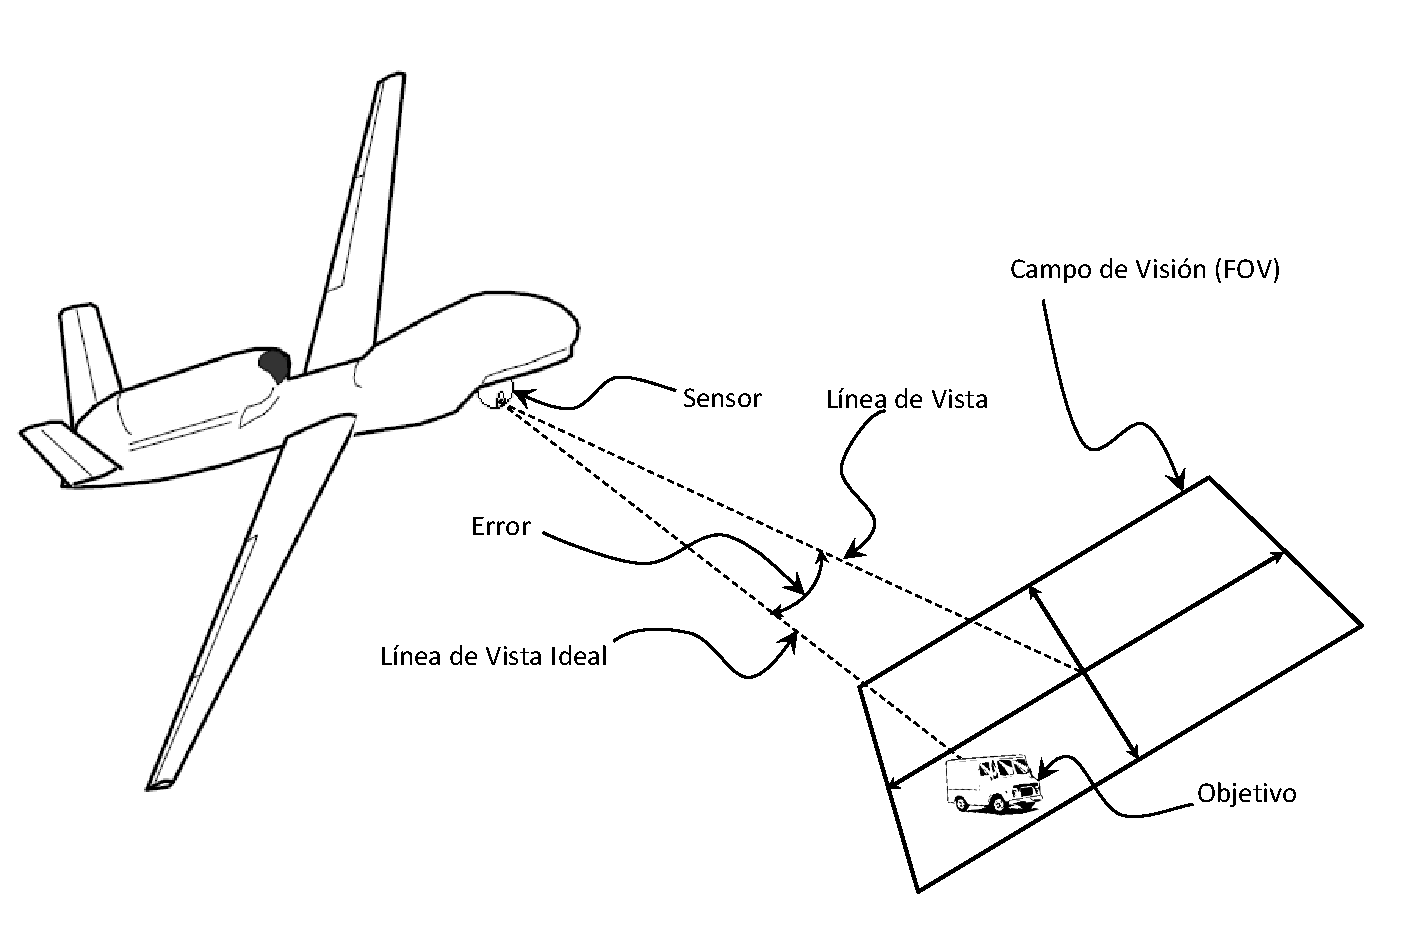
\includegraphics[scale=0.5]{img/LOSDef.pdf}
%trim = izquierda abajo derecha arriba
\caption{Definici\'{o}n de la L\'{i}nea de Vista}%Esta es la l\'{i}nea para el pie de figura
\label{fig:LOSDef}
\end{figure}

Entonces considerando lo mencionado anteriormente, podemos definir la estabilizaci\'{o}n de l\'{i}nea de vista como el acto de mantener el objetivo en el centro del campo de visi\'{o}n del sensor \'{o}ptico, bajo movimientos arbitrarios de la plataforma portadora del sistema y/o movimientos del objetivo a seguir. Se asume que la plataforma y el objetivo pueden moverse en los seis grados de libertad que definen la posici\'{o}n y orientaci\'{o}n de un cuerpo r\'{i}gido en el espacio tridimensional, que se definen por tres componentes de traslaci\'{o}n en tres ejes perpendiculares que describen los movimientos delante/atr\'{a}s, arriba/abajo e izquierda/derecha, combinados tres componentes de rotaci\'{o}n sobre los mismos tres ejes perpendiculares los cuales son com\'{u}nmente denominados en ingl\'{e}s como roll pitch y yaw, los cuales son conocidos como \'{a}ngulos n\'{a}uticos ya que son usados para describir la orientaci\'{o}n de una embarcaci\'{o}n o aeronave. Sin embargo el vector de la l\'{i}nea de vista tiene \'{u}nicamente dos grados de libertad debido a que la estabilizaci\'{o}n de l\'{i}nea de vista est\'{a} restringida al centro del campo de visi\'{o}n del sensor, en este contexto es posible que el objetivo se traslade y rote sobre el vector de la l\'{i}nea de vista y a\'{u}n as\'{i} satisfacer el prop\'{o}sito de estabilizaci\'{o}n. Un un sistema mec\'{a}nico capaz de mantener los dos \'{a}ngulos que definen el vector de l\'{i}nea de vista ideal es un sistema gimbal de dos ejes, el cual al rota el sensor alrededor de dos articulaciones angulares ortogonales que com\'{u}nmente consisten en un arreglo yaw/pitch.

Los dos marcos de referencia comunes para el mecanismo de estabilizaci\'{o}n son el marco inercial y el del campo de visi\'{o}n del sensor, estos se usan para medir el error entre la l\'{i}nea de vista medida y la deseada la cual centra el objetivo en el centro del campo de visi\'{o}n. La forma m\'{a}s com\'{u}n de estabilizaci\'{o}n de l\'{i}nea de vista consiste en medir las perturbaciones de la l\'{i}nea de vista en el marco inercial por medio de sensores inerciales. Esta informaci\'{o}n despu\'{e}s es usada en el sistema que controla los \'{a}ngulos de los eslabones del mecanismo de estabilizaci\'{o}n  para contrarrestar los movimientos del veh\'{i}culo y as\'{i} mantener fija l\'{i}nea de vista en el objetivo. Otro m\'{e}todo para estabilizar la l\'{i}nea de vista es medir la desviaci\'{o}n del objetivo del centro del campo de visi\'{o}n al procesar por medio de algoritmos de visi\'{o}n el v\'{i}deo obtenido por el sensor \'{o}ptico. Este m\'{e}todo es llamado "seguimiento de objetivo" y aunque en principio este m\'{e}todo parezca simple, en realidad tiene complicaciones importantes ya que se requiere un conocimiento preciso del campo de visi\'{o}n de la c\'{a}mara, una capacidad de procesamiento significativa para seguir el objetivo en tiempo real bajo variedad de condiciones de luz, y la trasformaci\'{o}n del error medido a las se\~{n}ales de control del sistema mec\'{a}nico \cite{26}. Este m\'{e}todo esta tambi\'{e}n sujeto a influencias externas tales como nubes que puedan obstruir el objetivo.

Los sistemas gimbal de estabilizaci\'{o}n de c\'{a}mara modernos combinan informaci\'{o}n obtenida de las mediciones de GPS, sensores inerciales, encoders, informaci\'{o}n de los estados del veh\'{i}culo e informaci\'{o}n de seguimiento de objetivo proveniente de una tarjeta de procesamiento de v\'{i}deo para generar una estabilizaci\'{o}n robusta.  
    



\section{Plataformas de Estabilizaci\'{o}n Inercial Aerotransportadas}

Las plataformas de estabilizaci\'{o}n inercial como se ha mencionado anteriormente, son usadas para estabilizar y apuntar un amplia variedad de sensores, c\'{a}maras, telescopios y sistemas de armas. Este tipo de sistemas se comenzaron a usarse desde hace aproximadamente cien a\~{n}os por lo que han sido usadas en todo tipo de veh\'{i}culos, desde sat\'{e}lites a submarinos e incluso en algunos dispositivos port\'{a}tiles \cite{29}. En especifico las plataformas de estabilizaci\'{o}n inercial aerotransportadas pueden ser de gran variedad de formas y tama\~{n}os las cuales generalmente est\'{a}n en funci\'{o}n del aeronave en la cual se montar\'{a}n para satisfacer un amplio rango de misiones y entre las cargas \'{u}tiles m\'{a}s comunes que se montan en una plataforma de estabilizaci\'{o}n inercial aerotransportada est\'{a}n:

\begin{itemize}
    \item Sistemas laser. (Tel\'{e}metros, Designadores)
    \item C\'{a}maras t\'{e}rmicas.
    \item C\'{a}maras electro \'{o}pticas de espectro visible.
    \item Antenas direccionales.   
\end{itemize}
La configuraci\'{o}n m\'{a}s com\'{u}n para un sistema gimbal de dos ejes es el llamado Pan-Tilt en el cual el primer eje, o el eje del eslab\'{o}n externo, permite la estabilizaci\'{o}n en el plano horizontal (paneo o acimut) mientras que el segundo eje, o el eje del eslab\'{o}n interno, permite la estabilizaci\'{o}n en el plano vertical (inclinaci\'{o}n o tilt). Las partes principales que componen un sistema de c\'{a}mara Pan-Tilt se muestran en la figura \ref{fig:CamParts}

\begin{figure}[H]
\centering 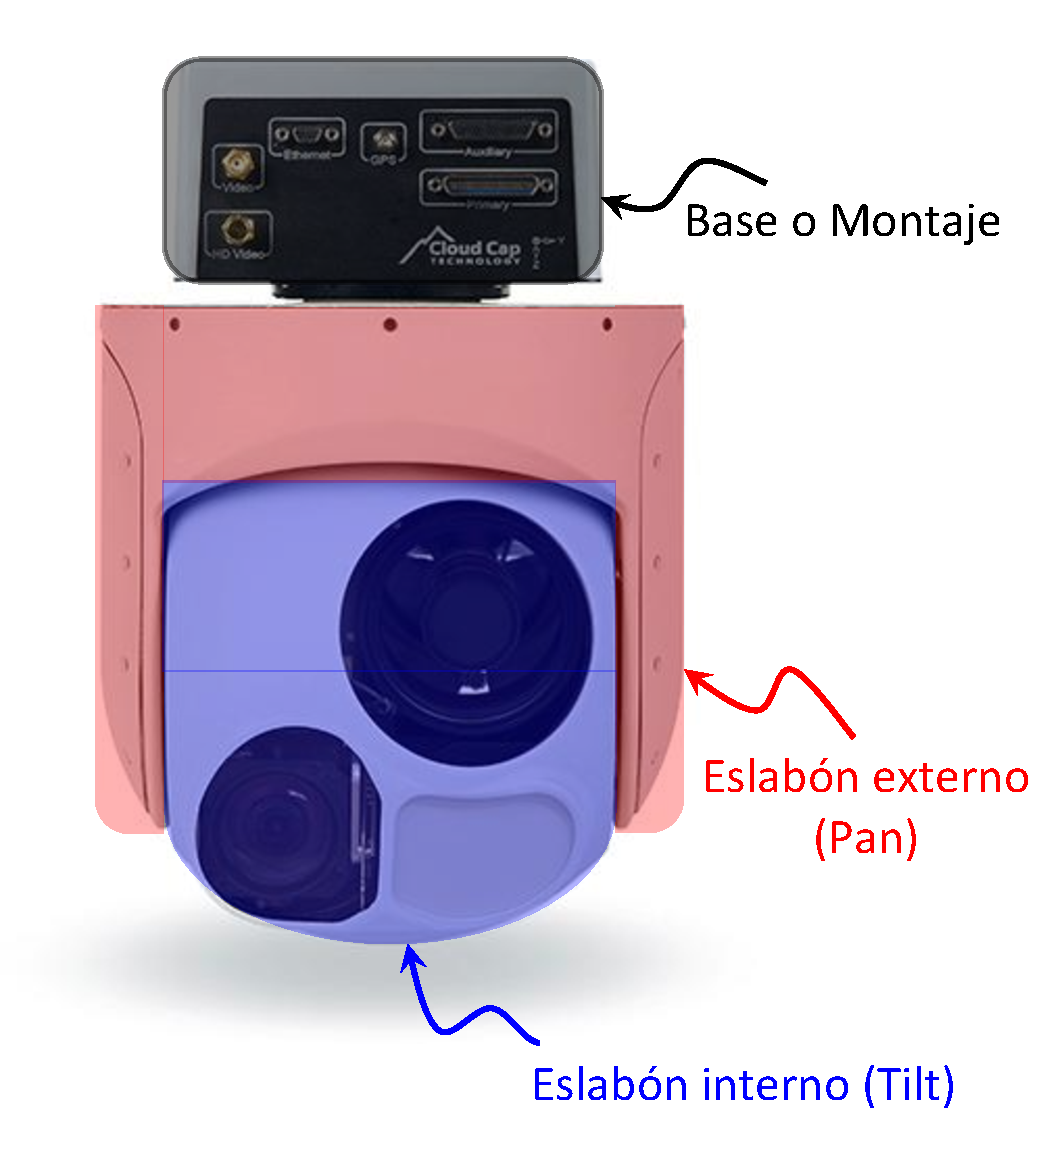
\includegraphics[scale=0.4]{img/GimbalParts.pdf}
%trim = izquierda abajo derecha arriba
\caption{Partes principales de un sistema de c\'{a}mara Pan-Tilt}%Esta es la l\'{i}nea para el pie de figura
\label{fig:CamParts}
\end{figure}

La base del gimbal es usualmente ligera y provee soporte estructural as\'{i} como aislamiento vibratorio al sistema gimbal mediante amortiguadores de vibraci\'{o}n de gel de silicio. El eslab\'{o}n externo provee a la c\'{a}mara de un movimiento de \textit{"paneo"} hacia la izquierda y derecha, el siguiente eslab\'{o}n, el interno lleva montada la carga \'{u}til y mueve la imagen de la c\'{a}mara hacia arriba y abajo (rotaci\'{o}n vertical) a \'{e}sta configuraci\'{o}n de gimbal se le conoce con diferentes nombres entre los cuales est\'{a}n: acimut/elevaci\'{o}n, pan/tilt o yaw/pitch La combinaci\'{o}n acimut/elevaci\'{o}n se refiere al horizonte terrestre y la combinaci\'{o}n yaw/pitch hace referencia a los \'{a}ngulos de n\'{a}uticos referenciados a un marco de referencia NED (Norte - Este - Abajo) por sus siglas en ingl\'{e}s. A lo largo de esta tesis usaremos la denominaci\'{o}n pan/tilt para referirnos a los \'{a}ngulos de los eslabones del gimbal.

Existe un amplio espectro de de sistemas gimbal, pero debido a que el uso de estos sistemas depende en gran medida de las capacidades de carga del aeronave que los transporta estos son clasificados principalmente en base a su peso total como: s\'{u}per ligeros, peque\~{n}os, medianos y grandes, en la figura ~\ref{fig:CamClases} se muestran ejemplos de sistemas gimbal ordenados seg\'{u}n su peso y tambi\'{e}n se muestra un ejemplo del tipo de aeronave capaz de llevar estos dispositivos, podemos concluir que un gimbal de mayor tama\~{n}o tendr\'{a} mayores capacidades de estabilizaci\'{o}n y m\'{a}s y mejores sensores, pero esto tambi\'{e}n incrementa las necesidades de un aeronave con mayor capacidad de carga.

\begin{figure}[h]
\centering 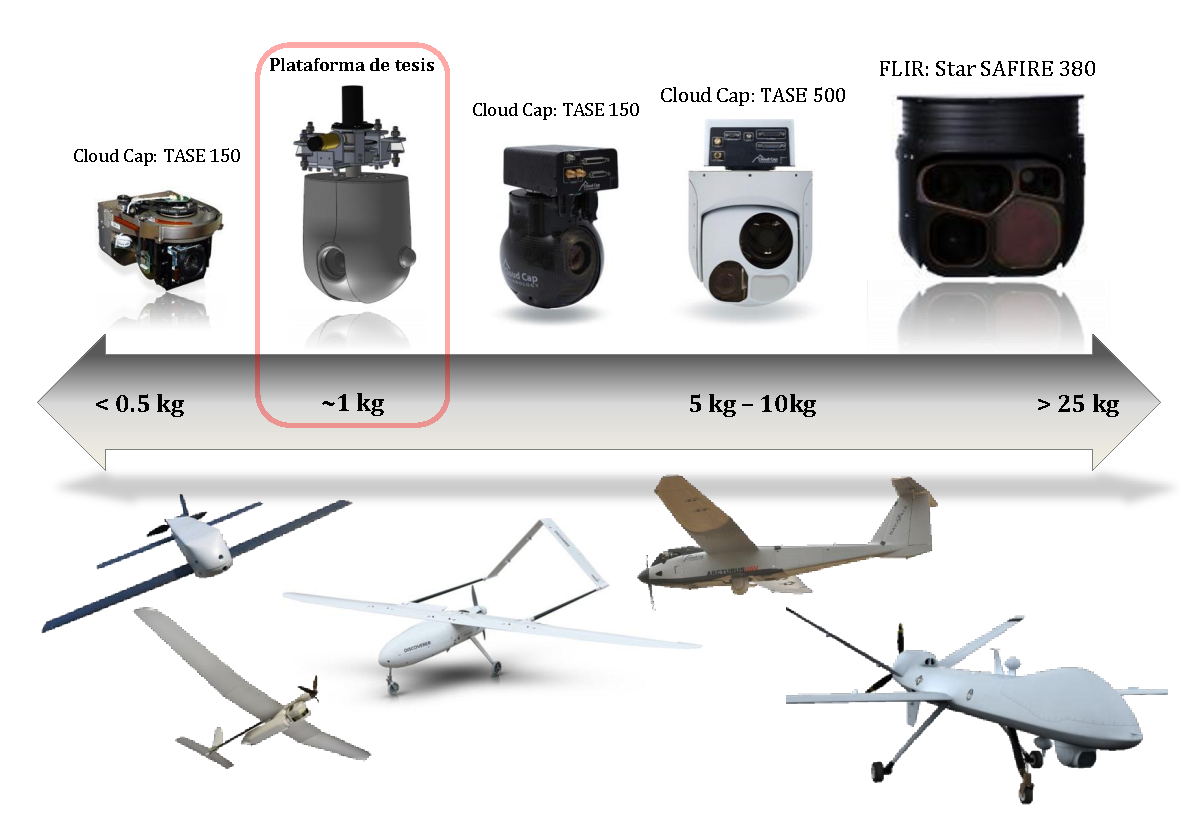
\includegraphics[scale=0.8]{img/Gimbalclases1.pdf}
%trim = izquierda abajo derecha arriba
\caption{Clasificaci\'{o}n de gimbals aerotransportados}%Esta es la l\'{i}nea para el pie de figura
\label{fig:CamClases}
\end{figure}

Los gimbals s\'{u}per ligeros, son aquellos qe tienen un peso de 0.5 kg o menos y son usado t\'{i}picamente por los vant's lanzados manualmente con un peso bruto de despegue m\'{a}ximo de alrededor de 2 a 5 kg. Estos gimbals pueden estabilizar una carga \'{u}til de hasta dos c\'{a}maras con dispositivo de carga acoplada (CCD) o una sola c\'{a}mara de bloque con zoom variable. Este tipo de gimbals son dise\~{n}ados espec\'{i}ficamente para la plataforma en la que ser\'{a}n utilizados y es necesario considerar que su forma afectar\'{a} su aerodin\'{a}mica, pues el sistema gimbal representar\'{a} una parte significativa de la superficie total del aeronave. la precisi\'{o}n en la estabilizaci\'{o}n de linea de vista alcanzada por estos dispositivos es t\'{i}picamente de $\pm0.5$ grados.

Los gimbals peque\~{n}os est\'{a}n en un rango de peso de entre los 0.5 y 5 kg. estos gimbals siguen teniendo limitaciones en su peso y forma, pero estos tienen una forma m\'{a}s cil\'{i}ndrica que permite el rango de movimiento completo que se aprecia en sistemas de mayor tama\~{n}o. Los gimbals de esta clase pueden com\'{u}nmente llevar dos tipos de cargas \'{u}tiles ofreciendo combinaciones interesantes en la resoluci\'{o}n del la c\'{a}mara y distancias focales. El error t\'{i}pico de los gimbals peque\~{n}os esta entre los $\pm0.5$ y los $\pm0.1$ grados.

Los sistemas de la clase media y grande, cuyos pesos van de los 5 a los 10 kg y mayores a los 25 kg respectivamente tienen una gran capacidad de combinaci\'{o}n de m\'{u}ltiples sensores. Estos sistemas son utilizados en veh\'{i}culos de gran autonom\'{i}a con intervalos de 8 a 24 horas y necesitan proveer al operador de un amplia variedad de opciones de captura de v\'{i}deo para manejar los cambios en las condiciones de luz que se presenten durante la duraci\'{o}n del vuelo. Estos gimbals tienen un error menor a los $\pm0.1$ grados pero est\'{a}n sometidos a una mayor exigencia debido la gran altitud que deben alcanzar las aeronaves que usan esta clase de sistemas ya que estas poseen grandes firmas ac\'{u}sticas\footnote{El t\'{e}rmino firma ac\'{u}stica es usado para describir las emisiones ac\'{u}sticas generadas por un aeronave y es de vital importancia para en aquellas aeronaves destinadas a misiones de vigilancia pues de este par\'{a}metro depende la altitud que ser\'{a} necesaria alcanzar para no ser detectado por el objetivo}.

\section{Integraci\'{o}n de los Sistemas de Estabilizaci\'{o}n Inercial}

En la integraci\'{o}n de un sistema gimbal en un aeronave no tripulada existen algunas cuestiones importantes que tienen que ser consideradas. Los veh\'{i}culos a\'{e}reos no tripulados se basan en un enlace de comunicaciones que envia comandos de mando y control al sistema gimbal. Debido a la latencia\footnote{En redes inform\'{a}ticas de datos se denomina latencia a la suma de retardos temporales dentro de una red. Un retardo es producido por la demora en la propagaci\'{o}n y transmisi\'{o}n de paquetes de datos dentro de la red.} y la calidad del enlace, los comandos pueden sufrir un retardo significativo desde el momento en el que el operador env\'{i}a los comandos y el sistema gimbal los recibe. 

\begin{figure}[H]
\centering 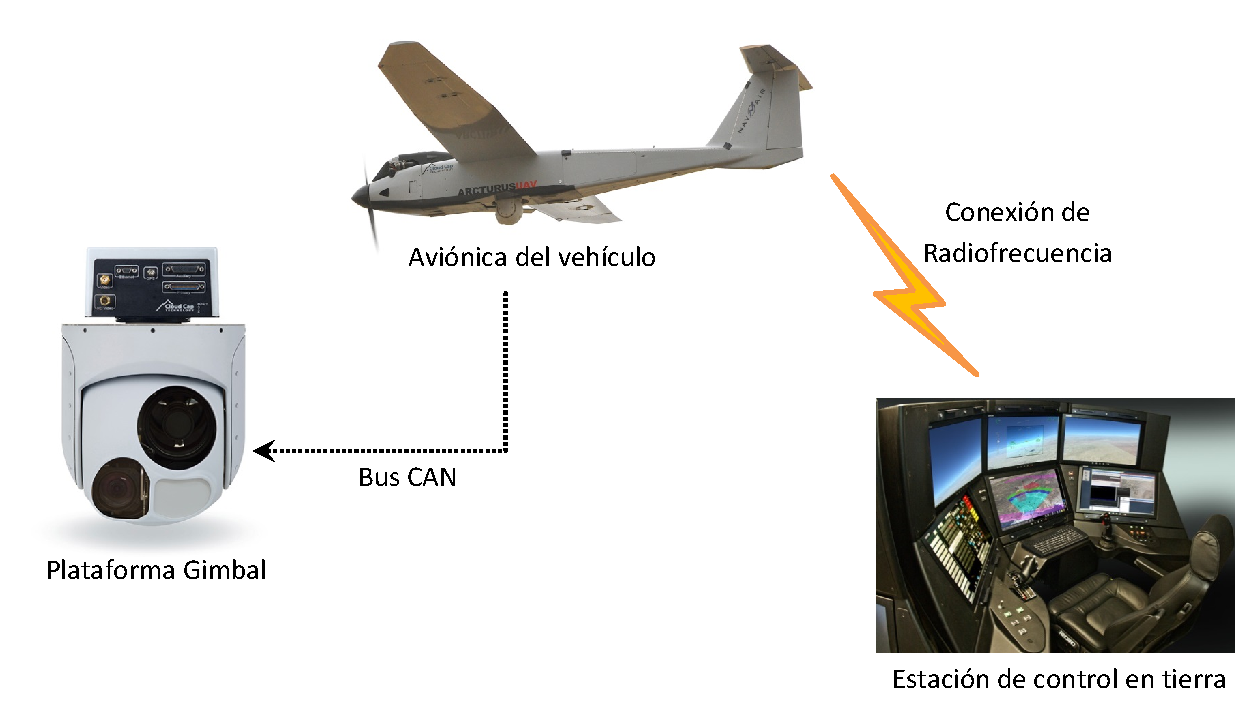
\includegraphics[scale=0.5]{img/integration.pdf}
%trim = izquierda abajo derecha arriba
\caption{Ejemplo de enlace de integraci\'{o}n gimbal-VANT}%Esta es la l\'{i}nea para el pie de figura
\label{fig:Integration}
\end{figure}

Estos retardos pueden dificultarle a un operador el seguimiento de un objetivo usando \'{u}nicamente un control manual, es por esto que caracter\'{i}sticas tales como se\~{n}alamiento a un punto GPS, seguimiento de trayectoria, e incluso triangulaci\'{o}n se integran a bordo del sistema gimbal y es com\'{u}n encontrar estas caracter\'{i}sticas en plataformas de gran tama\~{n}o, sin embargo, recientemente estas caracter\'{i}sticas comienzan a aparecer en sistemas m\'{a}s peque\~{n}os gracias al incremento de poder de procesamiento de los sistemas electr\'{o}nicos.

Los sistemas a\'{e}reos no tripulados (SANTs) deben proveer una conexi\'{o}n de datos bidirecional entre el operador y el gimbal para comando y control as\'{i} como para monitorear su estado. En los sistemas comerciales existe una tendencia a usar un protocolo CAN\footnote{CAN (acr\'{o}nimo del ingl\'{e}s Controller Area Network) es un protocolo de comunicaciones desarrollado por la firma alemana Robert Bosch GmbH, basado en una topolog\'{i}a bus para la transmisi\'{o}n de mensajes en entornos distribuidos} para la comunicaci\'{o}n entre el sistema de estabilizaci\'{o}n y la avi\'{o}nica del veh\'{i}culo. Los SANTs deben tambi\'{e}n proveer una conexi\'{o}n de datos que pueda transmitir el v\'{i}deo obtenido en tiempo real al operador. Se ha determinado por medio de pruebas, que una latencia mayor de 100-250ms entre el env\'{i}o del comando y la respuesta mostrada en el v\'{i}deo reduce significativamente la efectividad del operador durante el control manual del sistema, existen varias maneras de reducir este problema, una de las cuales es mejorar la conexi\'{o}n de datos al usar transmisores y receptores de mayor potencia para reducir la latencia, sin embargo esto no siempre es posible adem\'{a}s de la existencia de l\'{i}mites intr\'{i}nsecos en los sistemas de telecomunicaciones, otro enfoque consiste en aumentar la autonom\'{i}a del gimbal al embarcar algoritmos de se\~{n}alamiento por coordenadas GPS o algoritmos seguimiento basados en visi\'{o}n, de tal manera que se incremente la m\'{a}xima latencia permitida al dotar al sistema gimbal de la capacidad de realizar tareas de forma aut\'{o}noma durante la espera de la recepci\'{o}n de un nuevo comando de control de parte del operador lo que provee una estabilizaci\'{o}n a largo plazo mucho m\'{a}s all\'{a} de \'{u}nicamente la estabilizaci\'{o}n inercial bajo control manual. 

Otro factor clave en la integraci\'{o}n del sistema gimbal es el entorno vibratorio al cual estar\'{a} expuesto. Las aeronaves que poseen la capacidad de carga \'{u}til en volumen y peso necesarias para llevar gimbals de clase media son com\'{u}nmente propulsados por motores de combisti\'{o}n interna de 2 a 4 tiempos los cuales producen grandes pulsos de par debido a la naturaleza no continua de su operaci\'{o}n. Estos pulsos de par est\'{a}n com\'{u}nmente en el rango de los 50-80Hz y sin un aislamiento vibratorio espec\'{i}fico, puede causar desenfoque en la imagen y fluctuaciones en el sistema de control. La propulsi\'{o}n de tipo el\'{e}ctrica proporciona un sistema de par continuo, por lo que su comportamiento vibratorio es de una frecuencia mucho mayor a los motores de combusti\'{o}n interna, este tipo de vibraciones son m\'{a}s f\'{a}ciles de amortiguar y tienen un menor efecto en la calidad de la imagen. Sin embargo estas est\'{a}n limitadas a llevar \'{u}nicamente cargas \'{u}tiles peque\~{n}as debido a las limitaciones energ\'{e}ticas de sus bater\'{i}as. Las aeronaves con propulsi\'{o}n el\'{e}ctrica tienen una ventaja adicional pues tienen una firma ac\'{u}stica significativamente menor, lo que permite al veh\'{i}culo volar m\'{a}s cerca del objetivo y con esto reducir los requerimientos de estabilizaci\'{o}n del sistema gimbal y en consecuencia tambi\'{e}n su tama\~{n}o .

\section{Entorno Operativo}

El sistema desarrollado en este trabajo esta dise\~{n}ado para operar en Veh\'{i}culos No Tripulados peque\~{n}os con una capacidad de carga de aproximadamente 1.5 kg. Las altitudes de crucero t\'{i}picas para estos veh\'{i}culos est\'{a}n entre los 150 a los 600 metros sobre nivel de suelo y con una velocidad de viento en calma de 50 a 110 km/h. Si bien esto representa una peque\~{n}a secci\'{o}n del espacio a\'{e}reo, esta es tambi\'{e}n una secci\'{o}n particularmente susceptible a turbulencias impredecibles. En este rango las corrientes de aire son afectadas por la geograf\'{i}a, construcciones humanas, calentamiento de la superficie terrestre, adicionalmente a las condiciones clim\'{a}ticas. 

Lo anterior implica que un veh\'{i}culo peque\~{n}o es m\'{a}s susceptible a las turbulencias lo cual eleva las exigencias de estabilizaci\'{o}n. La baja inercia, carga alar y masa reducida a\~{n}ade vulnerabilidad a las turbulencias a los VANTs peque\~{n}os. En \cite{26} se obtienen datos de emp\'{i}ricos a partir de pruebas de vuelo en un VANT peque\~{n}o con un autopiloto trabajando a una frecuencia de 10Hz. En los resultados de estas pruebas se observa que aproximadamente el 99\% del tiempo de vuelo, la velocidad angular de veh\'{i}culo es de 2 rad/seg o menor. Estos datos son \'{u}tiles al elegir las perturbaciones a las que expone el modelo para el dise\~{n}o del algoritmo de control en las simulaci\'{o}nes desarrolladas en el cap\'{i}tulo ~\ref{sec:ControlChapter}. 

\section{Revisi\'{o}n Bibliogr\'{a}fica} 

En esta tesis se estudia la configuraci\'{o}n de un gimbal de dos ejes Pan-Tilt as\'{i} como un m\'{e}todo para la estabilizaci\'{o}n de la l\'{i}nea de vista, este tema ya ha sido discutido y analizado en muchos estudios previos bajo diferentes consideraciones y m\'{e}todos. En \cite{8}, \cite{9}, A.K. Rue realiza algunos de los primeros trabajos de investigaci\'{o}n sobre el tema siendo de las referencias m\'{a}s antiguas, en estos trabajos se obtiene y estudia la din\'{a}mica y el acoplamiento geom\'{e}trico de un mecanismo gimbal de dos ejes para el caso simplificado en el que los elementos del gimbal est\'{a}n balanceados y suspendidos sobre los ejes principales de inercia.  


En \cite{3}, Peter J. Kennedy desarrolla el modelo de un sistema gimbal de dos ejes, bajo la hip\'{o}tesis que cada eslab\'{o}n esta balanceado y que los ejes de rotaci\'{o}n est\'{a}n alineados con los ejes principales de inercia, tambi\'{e}n se estudian a fondo dos arquitecturas de control de estabilizaci\'{o}n, la directa y la indirecta, concluyendo que el enfoque directo es el que mejor desempe\~{n}o tiene. En \cite{4}, Ekstrand desarrolla el modelo del gimbal de dos grados de libertad empleando las ecuaciones de cuerpos r\'{i}gidos de Euler as\'{i} como el m\'{e}todo de Lagrange y demostr\'{o} que la mayor\'{i}a de las perturbaciones inerciales pueden ser eliminadas bajo ciertas condiciones de simetr\'{i}a. En \cite{5}, M. Abdo, desarroll\'{o} las ecuaciones de movimiento para el caso en el que existen masas no balanceadas en el sistema, es decir las matrices de inercia no son diagonales, esto con el objetivo de estudiar los efectos del acoplamiento cruzado, adem\'{a}s en \cite{6} dise\~{n}a un lazo de control PID en cascada para el control del sistema y prueba por medio de simulaci\'{o}n el desempe\~{n}o del algoritmo de control dise\~{n}ado. En \cite{10} se estudia el efecto de las perturbaciones no lineales debidas a la fricci\'{o}n y proponen un algoritmo LQR basado en una ecuaci\'{o}n diferencial linear de primer orden para estimar y compensar tales perturbaciones obteniendo un desempe\~{n}o considerablemente superior a un PI convencional. En \cite{11} se aborda el problema de la presencia de    incertidumbres en los par\'{a}metros de la fricci\'{o}n del motor desarrollando un m\'{e}todo para mejorar la convergencia del sistema basado en control \'{o}ptimo.

En la literatura, se han desarrollado y dise\~{n}ado sistemas de control para los sistemas gimbal de dos grados de libertad aplicando diferentes m\'{e}todos de control incluyendo el tratado a fondo en esta tesis, es decir el control por modos deslizantes. En \cite{12} se presenta una propuesta de control por modos deslizantes basado en un observador PI, mientras que en \cite{13} se desarrolla un control por modos deslizantes bajo la consideraci\'{o}n de canales id\'{e}nticos de elevaci\'{o}n y paneo. En \cite{14}, se propone un control por modos deslizantes \textit{"Proxy-based"} el cual es un un control por modos deslizantes adaptado al entorno discreto introducido por Kikuuwe y Fujimoto en el 2006 para control de robots. Adem\'{a}s de las t\'{e}cnicas de control convencionales tambi\'{e}n se han realizado investigaciones aplicando algunas t\'{e}cnicas avanzadas entre las cuales podemos mencionar al control adaptable por redes neuronales desarrollado en \cite{15}, al control robusto por din\'{a}mica inversa \cite{16}, Control por l\'{o}gica difusa en \cite{17} y a la metodolog\'{i}a de control robusto H$\infty$ \cite{18}, sin embrago la mayor\'{i}a de estas t\'{e}cnicas avanzadas son complejas y dif\'{i}ciles de implementar.  %Antecedentes
\chapter{Din\'{a}mica y Cinem\'{a}tica}\label{sec:Modelado}

\section{Descripci\'{o}n del Sistema}\label{sec:desdelsist}



Para desarrollar el modelo matem\'{a}tico del gimbal definiremos cuatro sistemas de coordenadas. Primeramente necesitamos un marco inercial,
para ello consideraremos la tierra como plana y estacionaria en un espacio
inercial, por lo que cualquier sistema coordenado o marco de referencia fijo en la misma es por ende un sistema inercial en el que las
leyes de newton son validas. Lo anterior es necesario para poder desarrollar
las ecuaciones de movimiento del gimbal de tal manera que denotaremos al
marco de referencia fijo en la tierra como el marco $\left( E\right) $
definido por los vectores unitarios $\left\{ \hat{I}_{E},\hat{J}_{E},%
\hat{K}_{E}\right\} ,$ donde su origen esta ubicado arbitrariamente en
la superficie de la tierra para ajustarse a las circunstancias del problema,
el eje $O_{E}\hat{K}_{E}$ apunta verticalmente hacia abajo y el eje $%
O_{E}\hat{I}_{E}$, el cual es horizontal se elije en cualquier direcci\'{o}n
conveniente, por ejemplo el norte o sobre un camino, o en alguna direccion
de referencia de vuelo.

Denotaremos el marco de referencia del cuerpo como $\left( B\right) $,
definido por los vectores unitarios $\left\{ \hat{\imath}_{B},\hat{\jmath}%
_{B},\hat{k}_{B}\right\} $ este marco esta fijo al fuselaje del aeronave
y consideraremos que se encuentra cerca de su centro de gravedad ver figura \ref{fig:RefFra}.

El marco que se encuentra fijo al eslab\'{o}n externo del gimbal lo
denotaremos como $\left( P\right) $, definido por el el conjunto de vectores
unitarios $\left\{ \hat{\imath}_{P},\hat{\jmath}_{P},\hat{k}_{P}\right\} 
$, este marco rota un \'{a}ngulo $ \eta $ alrededor del eje $\hat{k}_{B}$%
, a esta rotaci\'{o}n se le denomina \textit{"panning"}\ que se refiere a
una rotaci\'{o}n en el plano horizontal (azimut) de la c\'{a}mara (rotaci%
\'{o}n de gui\~{n}ada o \textit{"yaw"} en el aeronave).

Finalmente definimos el marco $\left( T\right) $ el cual es el marco de
referencia del eslab\'{o}n interno del gimbal y esta definido por los
vectores unitarios $\left\{ \hat{\imath}_{T},\hat{\jmath}_{T},\hat{k}%
_{T}\right\} $, este eslab\'{o}n rota un \'{a}ngulo $\varepsilon $ alrededor
del eje $\hat{\jmath}_{P}$ del eslab\'{o}n externo, esta rotaci\'{o}n es
denominada como elevaci\'{o}n o "tilting" que se refiere a una rotaci\'{o}n
de la camara en un plano vertical (rotaci\'{o}n de cabeceo o \textit{"pitch"}
en el aeronave).

\begin{figure}[thpb]
      \centering
      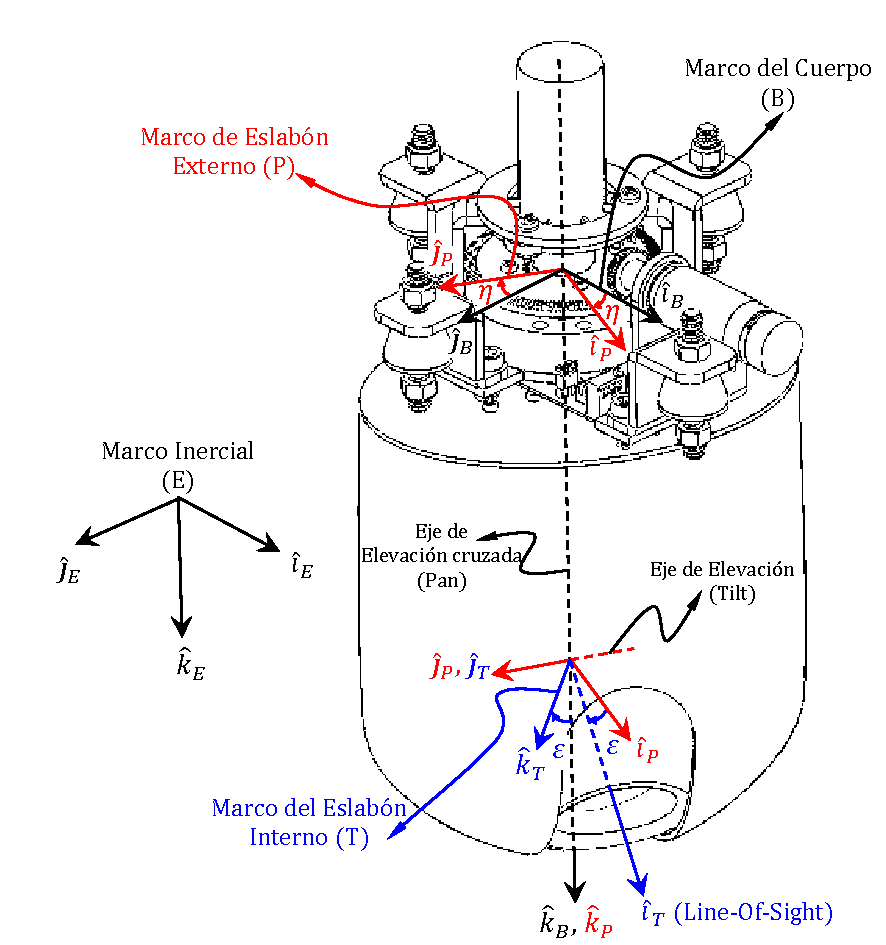
\includegraphics[scale=0.7]{img/Gimbal_Frames.pdf}
      \caption{Marcos de referencia del sistema gimbal}
      \label{fig:RefFra}
   \end{figure}

\section{Cin\'{e}matica}

Las velocidades \'{a}ngulares de los marcos $\left( P\right) $ y $\left(
T\right) $ son nuestras variables a controlar, el control de elevaci\'{o}n
se hace a traves del eslav\'{o}n interno, mientras que el control en el
plano horizontal (azimut) se hace a traves del eslab\'{o}n externo. Es
importante notar que la estabilizaci\'{o}n se requiere en el eje $\hat{\jmath%
}_{T}$ del eslab\'{o}n interno del gimbal denominado \textit{"elevaci\'{o}n
transversal"}; la estabilizaci\'{o}n se necesita en este eje puesto que es
en donde esta montada la c\'{a}mara, pero como antes se menciono la rotaci%
\'{o}n en azimut se controla con el eslab\'{o}n externo por lo que en
realidad la elevaci\'{o}n transversal es controlada indirectamente ya que el actuador esta montado en el eje $\hat{k}_{P}$ del eslab\'{o}n externo.

\subsection{Transformaciones b\'{a}sicas entre marcos de referencia}

Todos los marcos de referencia est\'{a}n relacionados por matrices de
transformaci\'{o}n, las cuales esta\'{a}n definidas como la suma de una matriz de traslaci\'{o}n
y una de rotaci\'{o}n. Considerando que nuestro inter\'{e}s se centra en velocidades \'{a} y aceleraciones \'{a}ngulares y \'{a}ngulos, y debido a que la
distancia que existe entre un marco y otro no afecta la forma en la que el
vector de velocidad de un marco se relaciona con otro, podemos despreciar esta distancia y considerar que el marco $%
\left( P\right) $ y $\left( T\right) $ tienen el mismo origen que $\left(
B\right) $ y de esta manera evitar utilizar la matriz de traslaci\'{o}n simplificando los c\'{a}lculos.

La matriz de rotaci\'{o}n que relaciona el marco de referencia $\left(
P\right) $ con respecto a $\left( B\right) $, la obtenemos calculando los
cosenos directores, de tal forma que:

\begin{equation*}
R_{B}^{P}=\left[ 
\begin{array}{lll}
\hat{\imath}_{P}\cdot \hat{\imath}_{B} & \hat{\jmath}_{P}\cdot \hat{\imath}%
_{B} & \hat{k}_{P}\cdot \hat{\imath}_{B} \\ 
\hat{\imath}_{P}\cdot \hat{\jmath}_{B} & \hat{\jmath}_{P}\cdot \hat{\jmath}%
_{B} & \hat{k}_{P}\cdot \hat{\jmath}_{B} \\ 
\hat{\imath}_{P}\cdot \hat{k}_{B} & \hat{\jmath}_{P}\cdot \hat{k}_{B}
& \hat{k}_{P}\cdot \hat{k}_{B}%
\end{array}%
\right]
\end{equation*}

\begin{equation*}
=\left[ 
\begin{array}{ccc}
\left\Vert \hat{\imath}_{P}\right\Vert \left\Vert \hat{\imath}%
_{B}\right\Vert \cos (\eta )\text{ \ \ \ \ \ \ \ } & \left\Vert \hat{\jmath}%
_{P}\right\Vert \left\Vert \hat{\imath}_{B}\right\Vert \cos (90+\eta ) & 
\left\Vert \hat{k}_{P}\right\Vert \left\Vert \hat{\imath}_{B}\right\Vert
\cos (90) \\ 
\left\Vert \hat{\imath}_{P}\right\Vert \left\Vert \hat{\jmath}%
_{B}\right\Vert \cos (90-\eta ) & \left\Vert \hat{\jmath}_{P}\right\Vert
\left\Vert \hat{\jmath}_{B}\right\Vert \cos (\eta )\text{ \ \ \ \ \ \ } & 
\left\Vert \hat{k}_{P}\right\Vert \left\Vert \hat{\jmath}_{B}\right\Vert
\cos (90) \\ 
\left\Vert \hat{\imath}_{P}\right\Vert \left\Vert \hat{k}_{B}\right\Vert
\cos (90)\text{ \ \ \ \ } & \left\Vert \hat{\jmath}_{P}\right\Vert
\left\Vert \hat{k}_{B}\right\Vert \cos (90)\text{ \ \ \ } & \left\Vert 
\hat{k}_{P}\right\Vert \left\Vert \hat{k}_{B}\right\Vert \cos (0)%
\text{ }%
\end{array}%
\right]
\end{equation*}

Usando la identidad trigonom\'{e}trica $\cos (a\pm b)=\cos (a)\cos (b)\mp \sin
(a)\sin (b)$:

\begin{equation*}
R_{B}^{P}=\left[ 
\begin{array}{ccc}
\cos (\eta )\text{ \ \ \ \ \ \ \ } & \cos (90)\cos (\eta )-\sin (90)\sin
(\eta ) & 0 \\ 
\cos (90)\cos (\eta )+\sin (90)\sin (\eta ) & \cos (\eta )\text{ \ \ \ \ \ \ 
} & 0 \\ 
0\text{\ \ \ } & 0\text{\ \ } & 1\text{ }%
\end{array}%
\right]
\end{equation*}

obtenemos finalmente:

\begin{equation}
R_{B}^{P}=\left[ 
\begin{array}{ccc}
c\eta & -s\eta & 0 \\ 
s\eta & c\eta & 0 \\ 
0\text{\ \ \ } & 0\text{\ \ } & 1\text{ }%
\end{array}%
\right] ;\text{ \ \ \ \ }c\eta =\cos (\eta );\text{ }s\eta =\sin (\eta )%
\text{\ \ }
\label{eq:R_P_B}
\end{equation}

Empleando las propiedades b\'{a}sicas de la matriz de rotaci\'{o}n,
obtenemos la relaci\'{o}n del marco de referencia $\left( B\right) $ con
respecto a $\left( P\right) $:

\begin{equation}
R_{P}^{B}=\left( R_{B}^{P}\right) ^{-1}=\left( R_{B}^{P}\right) ^{T}=\left[ 
\begin{array}{ccc}
c\eta & s\eta & 0 \\ 
-s\eta & c\eta & 0 \\ 
0\text{\ \ \ } & 0\text{\ \ } & 1\text{ }%
\end{array}%
\right]
\label{eq:R_B_P}
\end{equation}

De la misma manera obtenemos a continuaci\'{o}n la relaci\'{o}n del marco de
referencia $\left( P\right) $ con respecto a $\left( T\right) $:

\begin{equation*}
R_{T}^{P}=\left[ 
\begin{array}{ccc}
\hat{\imath}_{T}\cdot \hat{\imath}_{P} & \hat{\jmath}_{T}\cdot \hat{\imath}%
_{P} & \hat{k}_{T}\cdot \hat{\imath}_{P} \\ 
\hat{\imath}_{T}\cdot \hat{\jmath}_{P} & \hat{\jmath}_{T}\cdot \hat{\jmath}%
_{P} & \hat{k}_{T}\cdot \hat{\jmath}_{P} \\ 
\hat{\imath}_{T}\cdot \hat{k}_{P} & \hat{\jmath}_{T}\cdot \hat{k}_{P}
& \hat{k}_{T}\cdot \hat{k}_{P}%
\end{array}%
\right]
\end{equation*}

\begin{equation*}
\left[ 
\begin{array}{ccc}
\left\Vert \hat{\imath}_{T}\right\Vert \left\Vert \hat{\imath}%
_{P}\right\Vert \cos (\varepsilon )\text{ \ \ \ \ \ \ \ \ \ \ \ } & 
\left\Vert \hat{\jmath}_{T}\right\Vert \left\Vert \hat{\imath}%
_{P}\right\Vert \cos (90)\text{ \ \ } & \left\Vert \hat{k}%
_{T}\right\Vert \left\Vert \hat{\imath}_{P}\right\Vert \cos (90+\varepsilon )
\\ 
\left\Vert \hat{\imath}_{T}\right\Vert \left\Vert \hat{\jmath}%
_{P}\right\Vert \cos (90)\text{ \ \ \ \ \ \ \ \ } & \left\Vert \hat{\jmath}%
_{T}\right\Vert \left\Vert \hat{\jmath}_{P}\right\Vert \cos (0)\text{ \ \ \ }
& \left\Vert \hat{k}_{T}\right\Vert \left\Vert \hat{\jmath}%
_{P}\right\Vert \cos (90)\text{ \ \ \ \ } \\ 
\left\Vert \hat{\imath}_{T}\right\Vert \left\Vert \hat{k}_{P}\right\Vert
\cos (90-\varepsilon ) & \left\Vert \hat{\jmath}_{T}\right\Vert \left\Vert 
\hat{k}_{P}\right\Vert \cos (90) & \left\Vert \hat{k}_{T}\right\Vert
\left\Vert \hat{k}_{P}\right\Vert \cos (\varepsilon )\text{ \ \ \ \ }%
\end{array}%
\right]
\end{equation*}

\begin{equation*}
=\left[ 
\begin{array}{ccc}
\cos (\varepsilon ) & 0 & \cos (90)\cos (\varepsilon )-\sin (90)\sin
(\varepsilon ) \\ 
0 & 1 & 0 \\ 
\cos (90)\cos (\varepsilon )+\sin (90)\sin (\varepsilon ) & 0 & \cos
(\varepsilon )%
\end{array}%
\right]
\end{equation*}

obtenemos finalmente:

\begin{equation}
R_{T}^{P}=\left[ 
\begin{array}{ccc}
c\varepsilon & 0 & -s\varepsilon \\ 
0 & 1 & 0 \\ 
s\varepsilon \text{\ \ \ } & 0\text{\ \ } & c\varepsilon%
\end{array}%
\right] ;\text{ \ \ \ \ }c\varepsilon =\cos (\varepsilon );\text{ }%
s\varepsilon =\sin (\varepsilon )\text{\ \ }
\label{eq:R_P_T}
\end{equation}

\begin{equation}
R_{P}^{T}=\left( R_{T}^{P}\right) ^{-1}=\left( R_{T}^{P}\right) ^{T}=\left[ 
\begin{array}{ccc}
c\varepsilon & 0 & s\varepsilon \\ 
0 & 1 & 0 \\ 
-s\varepsilon \text{\ \ \ } & 0\text{\ \ } & c\varepsilon%
\end{array}%
\right]
\label{eq:R_T_P}
\end{equation}

\subsection{C\'{a}lculo de las velocidades angulares relativas}

Nuestro objetivo en esta secci\'{o}n es encontrar la definici\'{o}n de las
velocidades angulares de los eslabones externo e interno del gimbal
relativas al marco inercial, en \cite[82-84]{10} se establece la ecuaci\'{o}n que  relaciona una secuencia de $n$ marcos de referencia en movimiento arbitrario con respecto a estos mismos:

\begin{equation}
\omega _{n/1}=\overset{n}{\underset{i=2}{\sum }}\omega _{n/i-1}
\label{eq:refarbitrarymotion}
\end{equation}

Donde:

\begin{eqnarray*}
\omega _{i/j} &=&\text{velocidad angular del marco }\left\{ \hat{\imath}_{i},%
\hat{\jmath}_{i},\hat{k}_{i}\right\} \\
&&\text{con respecto al marco }\left\{ \hat{\imath}_{j},\hat{\jmath}_{j},%
\hat{k}_{j}\right\}
\end{eqnarray*}

Anteriormente hemos definido cuatro marcos de referencia $\left( E\right) $, 
$\left( B\right) $, $\left( P\right) $ y $\left( T\right) $, tomandolos
respectivamente como 1, 2, 3 y 4, y aplicando la ecuaci\'{o}n~\ref{eq:refarbitrarymotion} para el
eslab\'{o}n externo, obtenemos:

\begin{equation}
\omega _{P}=R_{P}^{B}\omega _{B}+\dot{\eta }\hat{k}_{P}
\label{eq:w_P}
\end{equation}

Donde $R_{P}^{B}\omega _{B}$ es la velocidad inercial del marco $\left( B\right) $ transformada al marco $\left( P\right) $ y el t\'{e}rmino $\dot{\eta }\hat{k}_{P}$ representa el movimiento relativo del marco $\left( P\right) $ con respecto al marco $\left( B\right) $, tal movimiento es \'{u}nicamente alrededor del eje $\hat{k}_{P}$.

Aplicando ahora la ecuaci\'{o}n ~\ref{eq:refarbitrarymotion} en el eslab\'{o}n interno, obtenemos:

\begin{equation}
\omega _{T}=R_{T}^{P}\omega _{P}+\dot{\varepsilon }\hat{\jmath}_{T}
\label{eq:w_T}
\end{equation}

Donde $R_{T}^{P}\omega _{P}$ es la velocidad inercial del marco $\left( P\right) $ transformada al marco $\left( T\right) $ y el t\'{e}rmino $\dot{\varepsilon }\hat{\jmath}_{T}$ representa el movimiento relativo del marco $\left( T\right) $ con respecto al marco $\left( P\right) $, tal movimiento es \'{u}nicamente alrededor del eje $\hat{\jmath}_{T}$.

\subsection{Relaciones cin\'{e}maticas b\'{a}sicas}\label{sec:RelCinBas}

Ahora a partir de las ecuaciones~\ref{eq:w_P} y~\ref{eq:w_T}, podemos obtener las ecuaciones que relacionan las velocidades angulares de los marcos de referencia definidos en la secci\'{o}n ~\ref{sec:desdelsist} entre estas, Dichas expresiones ser\'{a}n de utilidad en las secciones siguientes. Expresando la ecuaci\'{o}n ~\ref{eq:w_P} en forma vectorial, obtenemos

\begin{equation}
\left[\begin{array}{c} \omega_{P_x} \\\omega_{P_y} \\ \omega_{P_z} \end{array}\right] =
\left[\begin{array}{ccc} c\eta & s\eta & 0 \\  -s\eta & c\eta & 0 \\  0\text{\ \ \ } & 0\text{\ \ } & 1\text{ }\end{array} \right]
\left[\begin{array}{c} \omega_{B_x} \\\omega_{B_y} \\ \omega_{B_z} \end{array}\right] +
\left[\begin{array}{c} 0 \\0 \\ \dot{\eta } \end{array}\right]
\label{eq:w_P_vectf}
\end{equation}


\begin{align}
\omega_{P_x} & =c \eta \, \omega_{B_x} + s \eta \, \omega_{B_y} \label{eq:w_Px} \\
\omega_{P_y} & = -s \eta \, \omega_{B_x} + c \eta \, \omega_{B_y} \label{eq:w_Py} \\
\omega_{P_z} & =\omega_{B_z} + \dot{\eta} \label{eq:w_Pz}
\end{align}
Despejando $\dot{\eta}$ de la ecuaci\'{o}n ~\ref{eq:w_Pz}, obtenemos
\begin{equation}
\dot{\eta }=\omega _{P_z}-\omega _{B_z}
\label{eq:eta_dot}
\end{equation}
Expresando la ecuaci\'{o}n ~\ref{eq:w_T} en forma vectorial, obtenemos
\begin{equation}
\left[\begin{array}{c} \omega_{T_x} \\\omega_{T_y} \\ \omega_{T_z} \end{array}\right] =
\left[  \begin{array}{ccc} c\varepsilon & 0 & -s\varepsilon \\  0 & 1 & 0 \\  s\varepsilon \text{\ \ \ } & 0\text{\ \ } & c\varepsilon \end{array}\right]
\left[\begin{array}{c} \omega_{P_x} \\\omega_{P_y} \\ \omega_{P_z} \end{array}\right] +
\left[\begin{array}{c} 0 \\  \dot{\varepsilon } \\ 0  \end{array}\right]
\label{eq:w_T_vectf}
\end{equation}

\begin{align}
\omega_{T_x} & =c \varepsilon \, \omega_{P_x} - s \varepsilon \, \omega_{P_z} \label{eq:w_Tx}\\
\omega_{T_y} & = \omega_{P_y} + \dot{\varepsilon} \label{eq:w_Ty}\\
\omega_{T_z} & =s \varepsilon \, \omega_{P_x} + c \varepsilon \, \omega_{P_z} \label{eq:w_Tz}
\end{align}
Despejando $\dot{\varepsilon}$ de la ecuaci\'{o}n ~\ref{eq:w_Ty}, obtenemos
\begin{equation}
\dot{\varepsilon }=\omega _{T_y}-\omega _{P_y}
\label{eq:varepsi_dot}
\end{equation}




\section{Din\'{a}mica}

\subsection{Ecuaci\'{o}n de movimiento de Euler}
El modelo din\'{a}mico del gimbal puede obtenerse de las relaciones de par sobre los ejes del eslab\'{o}n interno y el externo del gimbal bas\'{a}ndose en la din\'{a}mica de cuerpo r\'{i}gido.

\begin{equation}
M=\frac{d H}{dt}+ \omega \times H
\label{eq:eulereq}
\end{equation}

Donde $M$ representa el momento aplicado, $d/dt$ es la derivada temporal en el marco del objeto y $H$ es el momento angular dado por
\begin{equation}
H=[I]\omega
\end{equation}

Considerando que los principales ejes de inercia coinciden con el marco de referencia, podemos considerar la matriz de inercia $I$ como una matriz diagonal, es decir

\begin{equation}
I = \left[ 
\begin{array}{ccc}
I_{x}  &      0   &   0 \\
   0     &  I_{y} &   0 \\
   0     &      0   & I_{z}\\
\end{array} \right]
\end{equation}

Realizando el producto vectorial definido en ~\ref{eq:eulereq}, obtenemos las tres ecuaciones escalares
\begin{equation}
\begin{array}{c}
M_{x}=I_{x}\dot{\omega}_{x}+\left(I_{z}-I_{y}\right)\omega _{y}\omega _{z}\\
M_{y}=I_{y}\dot{\omega}_{y}+\left(I_{x}-I_{z}\right)\omega _{x}\omega _{z}\\
M_{z}=I_{z}\dot{\omega}_{z}+\left(I_{y}-I_{x}\right)\omega _{x}\omega _{y}
\end{array}
\label{eq:euler}
\end{equation}
Las ecuaciones~\ref{eq:euler} son llamadas \textit{"ecuaciones de euler"} y ser\'{a}n las usadas para desarrollar las ecuaciones de movimiento del eslab\'{o}n interno y externo del gimbal.

\subsection{Fricci\'{o}n}\label{sec:friccion}

La fricci\'{o}n entre componentes m\'{o}viles no solo varia con el tiempo sino que tambi\'{e}n es de naturaleza no linear, tales fuerzas no deseadas son resultado del movimiento relativo de dos componentes que no han sido perfectamente aislados entre ellos, en nuestro caso de estudio, la fricci\'{o}n esta presente en los rodamientos sobre los que giran los ejes de los eslabones externo e interno del gimbal y se acent\'{u}a en los cambios en el sentido de rotaci\'{o}n. 
Las fuerzas de fricci\'{o}n pueden ser separadas en dos tipos: fricci\'{o}n de Coulomb y fricci\'{o}n viscosa. La fricci\'{o}n viscosa es proporcional a la velocidad relativa entre dos objetos y la fricci\'{o}n de Coulomb esta basada en el componente de fricci\'{o}n entre dos objetos debida a la fuerza normal aplicada y es no lineal en naturaleza, considerando lo anterior nuestro modelo de fricci\'{o}n puede expresarse como

\begin{equation}
T_{friccion}=T_{fviscosa}+T_{fcoulomb}
\end{equation}

Donde, para el eslab\'{o}n interno

\begin{equation*}
\begin{array}{c}
T_{fviscosa}=k_{Tvf} \, \dot{\varepsilon }\\

T_{fcoulomb}=k_{Tcf} \, \mathrm{sign}\left( \dot{\varepsilon} \right)
\end{array}
\end{equation*}
    

\subsection{Din\'{a}mica de elevaci\'{o}n (Tilting)}

Ahora analizaremos la din\'{a}mica del eslab\'{o}n interno o \textit{elevaci\'{o}n}. La matriz de inercia del eslab\'{o}n interno, esta dada por

\begin{equation}
I_T = \left[ 
\begin{array}{ccc}
I_{T_x}  &      0   &   0 \\
   0     &  I_{T_y} &   0 \\
   0     &      0   & I_{T_z}\\
\end{array} \right]
\end{equation}

Asumiendo que los ejes principales de inercia est\'{a}n alineados con los ejes de rotaci\'{o}n de tal manera que los productos de inercia se cancelan por lo cual podemos considerar la matriz de inercia como diagonal. La suma de torques externos sobre el eslab\'{o}n interno es 

\begin{equation}
M_T=\left[
\begin{array}{c}
T_{R_{Tx}} \\ T_{el} \\ T_{R_{Tz}}
\end{array}\right] -
\left[\begin{array}{c}
T_{U_{Tx}} \\ T_{U_{Ty}} \\ T_{U_{Tz}}
\end{array}\right]-
\left[
\begin{array}{c}
0 \\ T_{f_{Ty}} \\ 0
\end{array} \right]
\label{eq:M_tilt}
\end{equation}

Donde
$\\T_{el}$: Torque de control de elevaci\'{o}n.
$\\T_{f_{Ty}}$: Torque generado por efecto de la fricci\'{o}n sobre el eje $\hat{\jmath}_{T}$.
$\\T_{R_{Tx}}, \, T_{R_{Tz}}$: Torques de reacci\'{o}n del eslab\'{o}n interno sobre el eslab\'{o}n externo.
$\\T_{U_{Tx}}, \, T_{U_{Ty}}, \, T_{U_{Tz}}$:  Torques debidos a masas no balanceadas y otras perturbaciones no lineales no consideradas en el modelado.\newline 

El torque de control de estabilizaci\'{o}n $T_{el}$ producido por el motor montado sobre el eje $\hat{\jmath}_{T}$ del eslab\'{o}n interno del gimbal consiste en dos partes las cuales llamaremos $T_{T\omega}$ y $T_{Tq}$. La variable $T_{T\omega}$ tiene la funci\'{o}n principal de cancelar las perturbaciones y as\'{i} nulificar la velocidad angular $\omega_{T_y}$, mientras que $T_{Tq}$ es el control de posici\'{o}n , es decir permite colocar el eslab\'{o}n interno en un determinado \'{a}ngulo deseado.

Aplicando las ecuaciones de Euler definidas en~\ref{eq:euler} al eslab\'{o}n interno y combin\'{a}ndolas con~\ref{eq:M_tilt}, obtenemos las ecuaciones de movimiento para el eslab\'{o}n interno

\begin{equation}
\begin{array}{ccl}
T_{R_{Tx}}&=&I_{T_x}\dot{\omega}_{T_x}+\left(I_{T_z}-I_{T_y}\right)\omega _{T_y}\omega _{T_z}+T_{U_{Tx}}\\
T_{el}&=&I_{T_y}\dot{\omega}_{T_y}+\left(I_{T_x}-I_{T_z}\right)\omega _{T_x}\omega _{T_z}+T_{U_{Ty}}+T_{f_{Ty}}\\
T_{R_{Tz}}&=&I_{T_z}\dot{\omega}_{T_z}+\left(I_{T_y}-I_{T_x}\right)\omega _{T_x}\omega _{T_y}+T_{U_{Tz}}
\end{array}
\label{eq:Tilt_eqmov}
\end{equation}

Considerando que la primer y tercer ecuacion de~\ref{eq:Tilt_eqmov} no tienen uso pr\'{a}ctico esto debido a que solo la rotaci\'{o}n sobre el eje $\hat{\jmath}_{T}$ esta actuada y aplicando la definici\'{o}n para la fuerza de fricci\'{o}n expuesta en la secci\'{o}n~\ref{sec:friccion}, obtenemos la din\'{a}mica de \textit{elevaci\'{o}n}, dada por

\begin{equation}
T_{el}=I_{T_y}\dot{\omega}_{T_y}+\left(I_{T_x}-I_{T_z}\right)\omega _{T_x}\omega _{T_z}+k_{Tvf} \, \dot{\varepsilon }+k_{Tcf} \, \mathrm{sign}\left( \dot{\varepsilon} \right)+T_{U_{Ty}}
\label{Elev_1}
\end{equation} 

Las entradas de la ecuaci\'{o}n~\ref{Elev_1} son las velocidades y aceleraciones angulares de la base, mientras que las variables de control son las velocidades angulares en el eslab\'{o}n interno ${\omega}_{T_y}$ y ${\omega}_{T_z}$ en el eje de elevaci\'{o}n y acimut correspondientemente, es conveniente expresar la ecuaci\'{o}n ~\ref{Elev_1} en estos t\'{e}rminos. Sustituyendo ~\ref{eq:varepsi_dot} y~\ref{eq:w_Tx_cv} en ~\ref{Elev_1}
\begin{equation}
\begin{array}{cl}
I_{T_y}\dot{\omega}_{T_y} = & -k_{Tvf} \, \omega_{T_y} + \left[ t\varepsilon \, \left(I_{T_x}-I_{T_z}\right) \right]\omega_{T_y}^2 + \left[ \frac{1}{c \varepsilon} \left(I_{T_z}-I_{T_x}\right) \right] \omega _{P_x}\omega _{T_z} \\
 & + k_{Tvf} \, \omega_{P_y} +  k_{Tcf} \, \mathrm{sign}\left( \omega_{T_y} - \omega_{P_y} \right) + T_{el} + T_{U_{Ty}}
\end{array}
\label{Elev_2}
\end{equation}

Ahora usando las relaciones ~\ref{eq:w_Px} y ~\ref{eq:w_Py} es posible representar la ecuaci\'{o}n ~\ref{Elev_2} en t\'{e}rminos de las variables de control y las perturbaciones de la base.

\begin{equation}
\begin{array}{cl}
I_{T_y}\dot{\omega}_{T_y} = & -k_{Tvf} \, \omega_{T_y} + \left[ t\varepsilon \, \left(I_{T_x}-I_{T_z}\right) \right]\omega_{T_y}^2 + \\
 &\left[ \frac{1}{c \varepsilon} \left(I_{T_z}-I_{T_x}\right) \right] \left[ c \eta \omega_{B_x} \omega _{T_z} + s \eta \omega_{B_y} \omega _{T_z} \right] + k_{Tvf} \, \left[ c \eta \omega_{B_y} - s \eta \omega_{B_x} \right] \\
 & -  k_{Tcf} \, \mathrm{sign}\left( \omega_{T_y} - c \eta \omega_{B_y} + s \eta \omega_{B_x} \right) + T_{el} + T_{U_{Ty}}
\end{array}
\label{eq:Elev}
\end{equation}

\subsection{Din\'{a}mica Deseada}\label{sec:DinDes}

Para analizar la din\'{a}mica del canal de elevaci\'{o}n en el sentido de las perturbaciones  que influyen su movimiento, podemos reescribir la ecuaci\'{o}n ~\ref{eq:Elev} de la siguiente manera 

\begin{equation}
I_{T_y}\dot{\omega}_{T_y} = T_I + T_F + T_{U_{Ty}} + T_{el}
\end{equation}

Donde

\begin{equation}
T_I=\left[ t\varepsilon \, \left(I_{T_x}-I_{T_z}\right) \right]\omega_{T_y}^2 + \left[ \frac{1}{c \varepsilon} \left(I_{T_z}-I_{T_x}\right) \right] \left[ c \eta \omega_{B_x} \omega _{T_z} + s \eta \omega_{B_y} \omega _{T_z} \right] 
\end{equation}

\begin{equation}
\begin{array}{cl}
T_F=&-k_{Tvf} \, \omega_{T_y} -  k_{Tcf} \, \mathrm{sign}\left( \omega_{T_y} - c \eta \omega_{B_y} + s \eta \omega_{B_x} \right)\\
 &+ k_{Tvf} \, \left[ c \eta \omega_{B_y} - s \eta \omega_{B_x} \right]
\end{array}
\end{equation}

Desde el punto de vista de la estabilizaci\'{o}n, los t\'{e}rminos $T_I$, $T_F$ y $T_{U_{Ty}}$ representan perturbaciones no deseadas que afectan el desempe\~{n}o del sistema, el t\'{e}rmino $T_I$ contiene los par\'{a}metros inerciales y podemos observar que al considerar una simetr\'{i}a en la distrubuci\'{o}n de masa, tal que se cumpla la condici\'{o}n

\begin{equation}
I_{T_x} = I_{T_z}
\label{eq:SimCond}
\end{equation}

El t\'{e}rmino $T_I$ se vuelve cero. El t\'{e}rmino $T_F$ representa los efectos provocados por la fricci\'{o}n en la din\'{a}mica del sistema y $T_{U_{Ty}}$ representa las perturbaciones debidas masas no balanceadas y otras preturbaciones externas no consideradas en el modelado. Si consideramos el caso ideal en el que las perturbaciones $T_F = T_{U_{Ty}} =0$, la ecuaci\'{o}n ~\ref{eq:Elev} se transforma en   

\begin{equation}
I_{T_y}\dot{\omega}_{T_y} = T_{el}
\label{eq:ElDinDes}
\end{equation}

La cual representa el comportamiento ideal del canal de elevaci\'{o}n pues la velocidad angular depende \'{u}nicamente del par generado por el motor, por lo tanto podemos decir que la ecuaci\'{o}n ~\ref{eq:ElDinDes} es la din\'{a}mica deseada, en el sentido en el que no hay perturbaciones externas que influencien el movimiento alrededor del eje de elevaci\'{o}n $\hat{\jmath}_T$, es decir, no importa los movimientos que la plataforma tenga, la velocidad angular del eslab\'{o}n interno $\omega_{T_y}$ no ser\'{a} afectada.    

\subsection{Acoplamiento Cruzado Elevaci\'{o}n}

De la ecuaci\'{o}n de la din\'{a}mica de elevaci\'{o}n ~\ref{Elev_1}, podemos definir

\begin{equation}
T_D=\left(I_{T_x}-I_{T_z}\right)\omega _{T_x}\omega _{T_z}
\end{equation}

Usando las relaciones ~\ref{eq:w_Tx} y ~\ref{eq:w_Tz}, la expresi\'{o}n anterior puede escribirse como

\begin{equation}
T_D=T_B+T_D
\end{equation}

Donde

\begin{equation}
T_B=\frac{1}{2}\left(I_{T_x}-I_{T_z}\right)s2\varepsilon \, {\omega _{P_x}}^2 + \left(I_{T_x}-I_{T_z}\right) c2\varepsilon \, \omega _{P_z}\omega _{P_x}
\end{equation}

\begin{equation}
T_C=-\frac{1}{2}\left(I_{T_x}-I_{T_z}\right)s2\varepsilon \, {\omega _{P_z}}^2 
\end{equation}

Analizando los t\'{e}rminos $T_B$ y $T_C$, es claro que el eslab\'{o}n externo puede influenciar el interno independientemente de los movimientos de la base. Supongamos que la base se encuentra en reposo, es decir $\omega _{B_x}=\omega _{B_y}=\omega _{B_z}=0$, entonces de ~\ref{eq:w_Px}-~\ref{eq:w_Pz} tenemos que $\omega _{P_x}=\omega _{P_y}=0$ y por lo tanto $T_B=0$, sin embargo $\omega _{P_z}$ y por lo tanto $T_C$ no son necesariamente iguales a cero; por lo tanto los movimientos del eslab\'{o}n externo pueden influenciar el eslab\'{o}n interno, incluso para el caso en el que la base no esta rotando. Desde el punto de vista de control, $T_C$ es el t\'{e}rmino de acoplamiento cruzado, mientras que $T_B$ representa las perturbaciones provocadas por el movimiento de la base.  

\subsection{Din\'{a}mica de Elevaci\'{o}n Transversal (Panning)} \label{sec:Din_cross}

De manera similar utilizaremos las ecuaciones de Euler para obtener la din\'{a}mica del eslab\'{o}n externo. 

\begin{equation}
M_P=\frac{d H_P}{dt}+ \omega_P \times H_P + \left[ M_T \right]_P
\label{CrossEl_1}
\end{equation}

Donde el t\'{e}rmino $\left[ M_T \right]_P$ denota el momento del eslab\'{o}n interno ejercido sobre el eslab\'{o}n externo transformado al marco $P$ por la matriz de rotaci\'{o}n ~\ref{eq:R_T_P}. Expandiendo la ecuaci\'{o}n ~\ref{CrossEl_1}, obtenemos
\begin{equation}
M_P=I_{P}\dot{\omega}_{P}+ \omega_P \times I_{P}\omega_P + R_{P}^{T} \left[  I_{T}\dot{\omega}_{T} + \omega _{T} \times I_{T}\omega_T \right]
\label{CrossEl_2}
\end{equation}

Al igual que con el eslab\'{o}n interno, asumiremos que los ejes principales de inercia est\'{a}n alineados con los ejes de rotaci\'{o}n, de tal manera que la matriz de inercia es tambi\'{e}n diagonal. Observamos que en la ecuaci\'{o}n ~\ref{CrossEl_2} aparece el t\'{e}rmino $\dot{\omega}_{P}$ el cual representa la aceleraci\'{o}n angular en el marco de referencia del eslab\'{o}n externo m\'{a}s conveniente expresar esto \'{u}nicamente en t\'{e}rminos del eslab\'{o}n interno, es decir, $\dot{\omega}_{T}$. Para obtener la relaci\'{o}n entre la aceleraci\'{o}n angular del eslab\'{o}n interno y del externo podemos diferenciar la ecuaci\'{o}n ~\ref{eq:w_T}, con el proceso desarrollado en el ap\'{e}ndice ~\ref{sec:A2}. Sustituyendo la ecuaci\'{o}n ~\ref{eq:dotw_P} en ~\ref{CrossEl_2}

\begin{equation}
M_P=I_{P}\left[ R_{P}^{T}\dot{\omega} _{T} - R_{P}^{T}R_{Aux}\omega _{P}\dot{\varepsilon } - R_{P}^{T}\ddot{E} \right]+ \omega_P \times I_{P}\omega_P + R_{P}^{T} \left[  I_{T}\dot{\omega}_{T} + \omega _{T} \times I_{T}\omega_T \right]
\label{CrossEl_3}
\end{equation}

Expandiendo la expresi\'{o}n anterior

\begin{equation}
\begin{array}{rcl}
M_P&=& \left[ I_{P} R_{P}^{T} + R_{P}^{T} I_{T} \right] \dot{\omega}_{T} + \omega_P \times I_{P}\omega_P  + R_{P}^{T}\left(\omega _{T} \times I_{T}\omega_T \right)\\
& & - I_{P}R_{P}^{T}R_{Aux}\omega _{P}\dot{\varepsilon } - I_{P} R_{P}^{T}\ddot{E} 
\end{array}
\label{CrossEl_4}
\end{equation}

La din\'{a}mica de la \textit{Elevaci\'{o}n cruzada} esta dada por el tercer elemento del vector ~\ref{CrossEl_4}, la expansi\'{o}n de los componentes de la ecuaci\'{o}n anterior, se detalla en el ap\'{e}ndice ~\ref{sec:A3}, sustituyendo las ecuaciones ~\ref{eq:Term_1} - \ref{eq:Term_5} en ~\ref{CrossEl_4}

\begin{equation}
\begin{array}{rcl}
\left[ M_P \right]_3&=&c\varepsilon \left( I_{P_z}+I_{T_z} \right)\dot{\omega}_{T_z} - s\varepsilon \left( I_{P_z}+I_{T_x} \right)\dot{\omega}_{T_x} + \left( I_{P_y}-I_{P_x} \right) \omega_{P_x} \omega_{P_y}\\
 & & - s\varepsilon I_{T_z} \omega_{T_y} \omega_{T_z} + I_{T_y} \omega_{T_y} \omega_{P_x} - c\varepsilon I_{T_x} \omega_{T_x} \omega_{T_y} - I_{P_z} \omega_{P_z}\dot{\varepsilon}
 \end{array}
 \label{CrossEl_5}
\end{equation}

La suma de los pares cin\'{e}maticos sobre el eslab\'{o}n externo esta dada por

\begin{equation}
M_P=\left[
\begin{array}{c}
T_{R_{Px}} \\ T_{R_{Py}} \\ T_{az}
\end{array}\right] -
\left[\begin{array}{c}
T_{U_{Px}} \\ T_{U_{Py}} \\ T_{U_{Pz}}
\end{array}\right]-
\left[
\begin{array}{c}
0 \\ 0 \\ T_{f_{Pz}}
\end{array} \right]
\label{eq:M_pan}
\end{equation}

Donde

$\\T_{az}$: Torque de control de acimut.
$\\T_{f_{Pz}}$: Torque generado por efecto de la fricci\'{o}n sobre el eje $\hat{k}_{P}$.
$\\T_{R_{Px}}, \, T_{R_{Py}}$: Torques de reacci\'{o}n del eslab\'{o}n externo sobre la plataforma.
$\\T_{U_{Tx}}, \, T_{U_{Ty}}, \, T_{U_{Tz}}$: Torques debidos a masas no balanceadas y otras perturbaciones no lineales no consideradas en el modelado.\newline 

De la misma manera como anteriormente, el torque de control de estabilizaci\'{o}n $T_{az}$ producido por el motor montado sobre el eje $\hat{k}_{T}$ del eslab\'{o}n interno del gimbal consiste en dos partes: La cancelaci\'{o}n de perturbaciones $T_{P\omega}$ y el posicionamiento $T_{Pq}$. Ya que la estabilizaci\'{o}n es requerida sobre el eje  
$\hat{k}_{P}$, llamado \textit{"elevaci\'{o}n cruzada"}, $T_{az}$ es usado para controlar indirectamente $\omega_{T_z}$, esto plantea un problema debido a las no linealidades que aparecen en el sistema din\'{a}mico. Combinando ~\ref{CrossEl_5} con ~\ref{eq:M_pan}, obtenemos

\begin{equation}
\begin{array}{rcl}
c\varepsilon \left( I_{P_z}+I_{T_z} \right)\dot{\omega}_{T_z}&=&s\varepsilon \left( I_{P_z}-I_{T_x} \right)\dot{\omega}_{T_x} + \left( I_{P_y}-I_{P_x} \right) \omega_{P_x} \omega_{P_y}- s\varepsilon I_{T_z} \omega_{T_y} \omega_{T_z}\\
 & &  + I_{T_y} \omega_{T_y} \omega_{P_x} - c\varepsilon I_{T_x} \omega_{T_x} \omega_{T_y} - I_{P_z} \omega_{P_z}\dot{\varepsilon}-T_{U_{Pz}}-T_{f_{Py}}+T_{az}
 \end{array}
 \label{CrossEl_6}
\end{equation}

En el anexo ~\ref{sec:A2} se obtuvieron las aceleraciones angulares a partir de la cinem\'{a}tica del gimbal, resolviendo ~\ref{eq:dotw_T} para $\dot{\omega}_{T_x}$ y sustituyendo en ~\ref{CrossEl_5}

\begin{equation}
\begin{array}{rcl}
Js\dot{\omega}_{T_z}&=&s\varepsilon \left( I_{P_z}-I_{T_x} \right)\dot{\omega}_{T_x} + \left[ I_{P_z} \omega_{T_x} - s\varepsilon I_{T_x} \omega_{P_z} \right]\dot{\varepsilon}\\

 & &-c\varepsilon\left[ \left( I_{P_y}-I_{P_x} \right) \omega_{P_x} \omega_{P_y}- s\varepsilon I_{T_z} \omega_{T_y} \omega_{T_z} + I_{T_y} \omega_{T_y} \omega_{P_x} - c\varepsilon I_{T_x} \omega_{T_x} \omega_{T_y}\right] \\
 
 & &  + c\varepsilon\left[T_{U_{Pz}}-k_{Pvf}\dot{\eta }+k_{Pcf} \, \mathrm{sign}\left( \dot{\eta} \right) + T_{az} \right]
 \end{array}
 \label{CrossEl_7}
\end{equation}

Donde

\begin{equation}
Js=I_{P_z} + c^2 \varepsilon I_{T_z} + s^2 \varepsilon I_{T_x}
\label{eq:PanTotInertia}
\end{equation}

El t\'{e}rmino $Js$ definido en ~\ref{eq:PanTotInertia} es el momento total de inercia del sistema gimbal sobre el eje $\hat{k}_P$ si el eslab\'{o}n interno del gimbal ha rotado un \'{a}ngulo $\varepsilon$. Sin embargo, incluso si el \'{a}ngulo $\varepsilon$ varia en el tiempo, $Js$ es el momento de inercia instant\'{a}neo sobre el eje $\hat{k}_P$.

Al igual que que con la din\'{a}mica de elevaci\'{o}n la ecuaci\'{o}n ~\ref{CrossEl_7} necesita ser expresada en t\'{e}rminos de de las variables controladas $\omega_{T_z}$, $\omega_{T_y}$, las perturbaciones de la base $\omega_{B}$, y los \'{a}ngulos de elevaci\'{o}n y azimut $\varepsilon$ y $\eta$. Finalmente, la expresi\'{o}n de la di\'{a}mica en t\'{e}rminos de las variables de inter\'{e}s se muestra en ecuaci\'{o}n ~\ref{CrossEl} y el desarrollo de \'{e}sta expresi\'{o}n se detalla en el ap\'{e}ndice ~\ref{sec:A4}

\begin{equation}
\begin{array}{rcl}
Js\dot{\omega}_{T_z} & = & -k_{Pvf} \omega_{T_z} +\left[s\varepsilon \, c\varepsilon\left(I_{T_z} -I_{T_x} \right) - t\varepsilon \left(I_{P_z} +I_{T_x} \right) \right]\omega_{T_y}\omega_{T_z} + \left[ 2t\varepsilon \left(I_{P_z} +I_{T_x} \right) \right] \\

 & & \left[c\eta \omega_{T_z}\omega_{B_y} - s\eta \omega_{T_z}\omega_{B_x}\right] +\left[ \frac{1}{c\varepsilon} \left(I_{P_z} +I_{T_x} \right)- c\varepsilon I_{T_y} \right] \left[ c\eta \omega_{T_y}\omega_{B_x} + s\eta \omega_{T_y}\omega_{B_y}\right]\\ 

 & & + \left[s\varepsilon \left(I_{P_z} +I_{T_x} \right)\right]\left[ c\eta\dot{\omega}_{B_x} + s\eta\dot{\omega}_{B_y}- c\eta\omega_{B_z}\omega_{By} + s\eta\omega_{B_z}\omega_{Bx}\right]\\
 
 & & +\left[c\varepsilon \left(I_{P_x} +I_{P_y} \right)- s\varepsilon \, t\varepsilon \left(I_{P_z} +2I_{T_x} \right)-\frac{1}{c\varepsilon}I_{P_z} \right]\\ 
 
 & &  \left[\left(c\eta \omega_{B_y}-s\eta \omega_{B_x}\right)\left(c\eta \omega_{B_x}-s\eta \omega_{B_y}\right)\right]\\ 
 
 & & + s\varepsilon k_{Pvf}\left(c\eta \omega_{B_x}-s\eta \omega_{B_y}\right) + c\varepsilon k_{Pvf}\omega_{B_z}\\ 
 
 & & - c\varepsilon k_{Pcf} \, \mathrm{sign}\left( \frac{1}{c\varepsilon} \omega_{T_z} - t\varepsilon c\eta \omega_{B_x}-t\varepsilon s\eta \omega_{B_y} - \omega_{B_z}\right)\\ 
 
 & & - c\varepsilon T_{U_{Pz}} +c\varepsilon T_{az}
 
\end{array}
\label{CrossEl}
\end{equation}

\subsection{Propiedades del Sistema}\label{sec:propiedadessist}

Comparado con el canal de elevaci\'{o}n, tenemos algunas diferencias importantes, las cuales restringen el desempe\~{n}o alcanzable por la configuraci\'{o}n Pan-tilt.

Podemos observar a partir de la ecuaci\'{o}n ~\ref{CrossEl_7} que existe un factor $\cos \left(\varepsilon \right)$ que afecta la ganancia en el lazo de control, es decir, la ganancia depende del \'{a}ngulo de elevaci\'{o}n $\varepsilon$. Tal dependencia en la ganancia del canal de elevaci\'{o}n puede resultar problem\'{a}tica ya que significa dificultades para obtener el ancho de banda requerido para diferentes \'{a}ngulos de elevaci\'{o}n. Una manera de manejar esto es dividir por $\cos \left(\varepsilon \right)$, es decir agregar al controlador in factor $\frac{1}{\cos \left(\varepsilon \right)}$. Si el \'{a}ngulo $\varepsilon$ cambia lentamente comparado con la constante de tiempo implicada, el cual es normalmente el caso, la dependencia ser\'{i}a casi eliminada.

Sin embargo, cuando $\varepsilon \rightarrow \frac{\pi}{2}$ este m\'{e}todo para compensar $\cos \left(\varepsilon \right)$ incrementar\'{a} la demanda en el par m\'{a}ximo del motor, y por supuesto no funcionar\'{a} para $\varepsilon = \frac{\pi}{2}$, pues en este punto se ha alcanzado un punto singular del sistema. El sistema gimbal, a\'{u}n y cuando funciona bien sobre casi todo su rango de operaci\'{o}n, se vuelve menos que ideal cuando la c\'{a}mara se orienta casi o directamente hacia abajo. Para rastrear objetivos que pasan a trav\'{e}s de la posici\'{o}n directamente bajo el avi\'{o}n se requiere de un movimiento muy r\'{a}pido alrededor del eje de acimut. Entre m\'{a}s cerca pase el objetivo del punto que est\'{a} directamente debajo del avi\'{o}n, el motor deber\'{a} girar m\'{a}s r\'{a}pido el eslab\'{o}n externo sobre el eje de acimut para rastrear el objetivo. Si el objetivo pasa directamente debajo del avi\'{o}n, el motor deber\'{i}a ser capaz de girar el eslab\'{o}n externo del gimbal a una velocidad infinita. De hecho, cualquier mecanismo de orientaci\'{o}n con dos grados de libertad que tenga exactamente dos articulaciones giratorias no puede evitar este problema. En este caso especial, cuando la l\'{i}nea de vista de la c\'{a}mara se dirige hacia un objetivo que pasa directamente debajo, su direcci\'{o}n se alinea con el eje de rotaci\'{o}n del eslab\'{o}n externo $\hat{k}_{P}$. Esto significa que, en este punto en particular, la rotaci\'{o}n en acimut no produce cambio alguno en la direcci\'{o}n en la que apunta la l\'{i}nea de vista. Sabemos que necesitamos dos grados de libertad para orientar la l\'{i}nea de vista, pero en este punto, hemos perdido el uso efectivo de una de las articulaciones. nuestro mecanismo se ha vuelto \textit{"localmente degenerado"} y se comporta como si solamente tuviera un grado de libertad (la direcci\'{o}n de elevaci\'{o}n), a esta regi\'{o}n cercana al punto singular se le llama \textit{"cono de oclusi\'{o}n"}. Por lo tanto, el punto de singularidad $\varepsilon = \frac{\pi}{2}$ y valores cercanos a este punto deben evitarse.

Podemos notar a partir de la ecuaci\'{o}n ~\ref{eq:PanTotInertia} que el factor $Js$ tambi\'{e}n tiene una dependencia con el \'{a}ngulo de elevaci\'{o}n $\varepsilon$, lo que genera una dependencia adicional de la ganancia del lazo con el \'{a}ngulo $\varepsilon$. Sin embargo si se cumple la condici\'{o}n de simetr\'{i}a ~\ref{eq:SimCond} la dependencia de $Js$ con el \'{a}ngulo $\varepsilon$ es eliminada, lo que denota la importancia de considerar la simetr\'{i}a de la distribuci\'{o}n de masa en el dise\~{n}o mec\'{a}nico del gimbal.

Hay dos tipos diferentes de perturbaciones que pueden influenciar la din\'{a}mica de la elevaci\'{o}n cruzada, las perturbaciones inerciales y las restricciones del sistema, las perturbaciones inerciales son aquellas en las que est\'{a}n involucrados los momentos y productos de inercia, los cuales como hemos observado en para el canal de elevaci\'{o}n, estas pueden eliminarse bajo adecuadas consideraciones de simetr\'{i}a. Esto significa que podemos pensar que la mayor\'{i}a de las perturbaciones inerciales son causadas por una distribuci\'{o}n asim\'{e}trica de la masa en el sistema gimbal. 

Por otro lado, las restricciones del sistema provienen principalmente del t\'{e}rmino $\omega_{P_x} \, \sin (\varepsilon)$ en la definici\'{o}n de $\omega_{T_z}$ (ecuaci\'{o}n~\ref{eq:w_Tz})y no pueden ser eliminadas bajo ninguna consideraci\'{o}n de simetr\'{i}a, ya que la inercia no esta involucrada en este t\'{e}rmino y tambi\'{e}n podemos notar que no tiene relaci\'{o}n con el canal de elevaci\'{o}n. Esta es una importante y problem\'{a}tica perturbaci\'{o}n generada por las rotaciones de la plataforma $\omega_{B_x}$ y $\omega_{B_y}$ que tienen una influencia directa en la salida. La atenuaci\'{o}n de tal perturbaci\'{o}n directa en la salida puede resultar complicada y requiere de un alto desempe\~{n}o del sistema de control.

   
 %Modelado
\chapter{Dise\~{n}o del Control de Estabilizaci\'{o}n} \label{sec:ControlChapter}

\section{Introducci�n}
El objetivo principal de este trabajo es implementar un control que permita la estabilizaci\'{o}n de l\'{i}nea de vista de la c\'{a}mara montada en el eslab\'{o}n interno del del sistema gimbal. El torque de control de elevaci�n $T_{el}$  y el torque de control de la elevaci�n cruzada $T_{az}$ pueden ser generados por diferentes algoritmos, pero indiferentemente del algoritmo el principal objetivo del sistema de control es suprimir cualquier efecto provocado por el movimiento del aeronave, es decir $\omega_{B}$ o su derivada  $\dot{\omega}_B$. Esto se puede lograr mediante realimentaci\'{o}n directa (Estabilizaci\'{o}n Directa) o mediante la cancelaci\'{o}n de la perturbaci\'{o}n por medio de las mediciones inerciales en la base del gimbal (Estabilizaci\'{o}n Indirecta). Para el dise\~{n}o del control del sistema se ha optado por elegir el enfoque de estabilizaci\'{o}n directa, ya que en el an\'{a}lisis desarrollado por P. J. Kennedy en \cite{3}, se concluye que con el m\'{e}todo de estabilizaci\'{o}n directa se pueden obtener mejores resultados en la estabilizaci\'{o}n de la l\'{i}nea de vista. En la estabilizaci\'{o}n directa, se miden las velocidades angulares $\omega_{T_y}$ y $\omega_{T_z}$ y estas son usadas para generar los torques de compensaci�n $T_{T\omega}$ y $T_{P\omega}$, los cuales intentan anular las perturbaciones medidas, la figura ~\ref{fig:BloquesCont} muestra la configuraci\'{o}n para el lazo de control de estabilizaci\'{o}n directa.

\begin{figure}[H]
\centering
      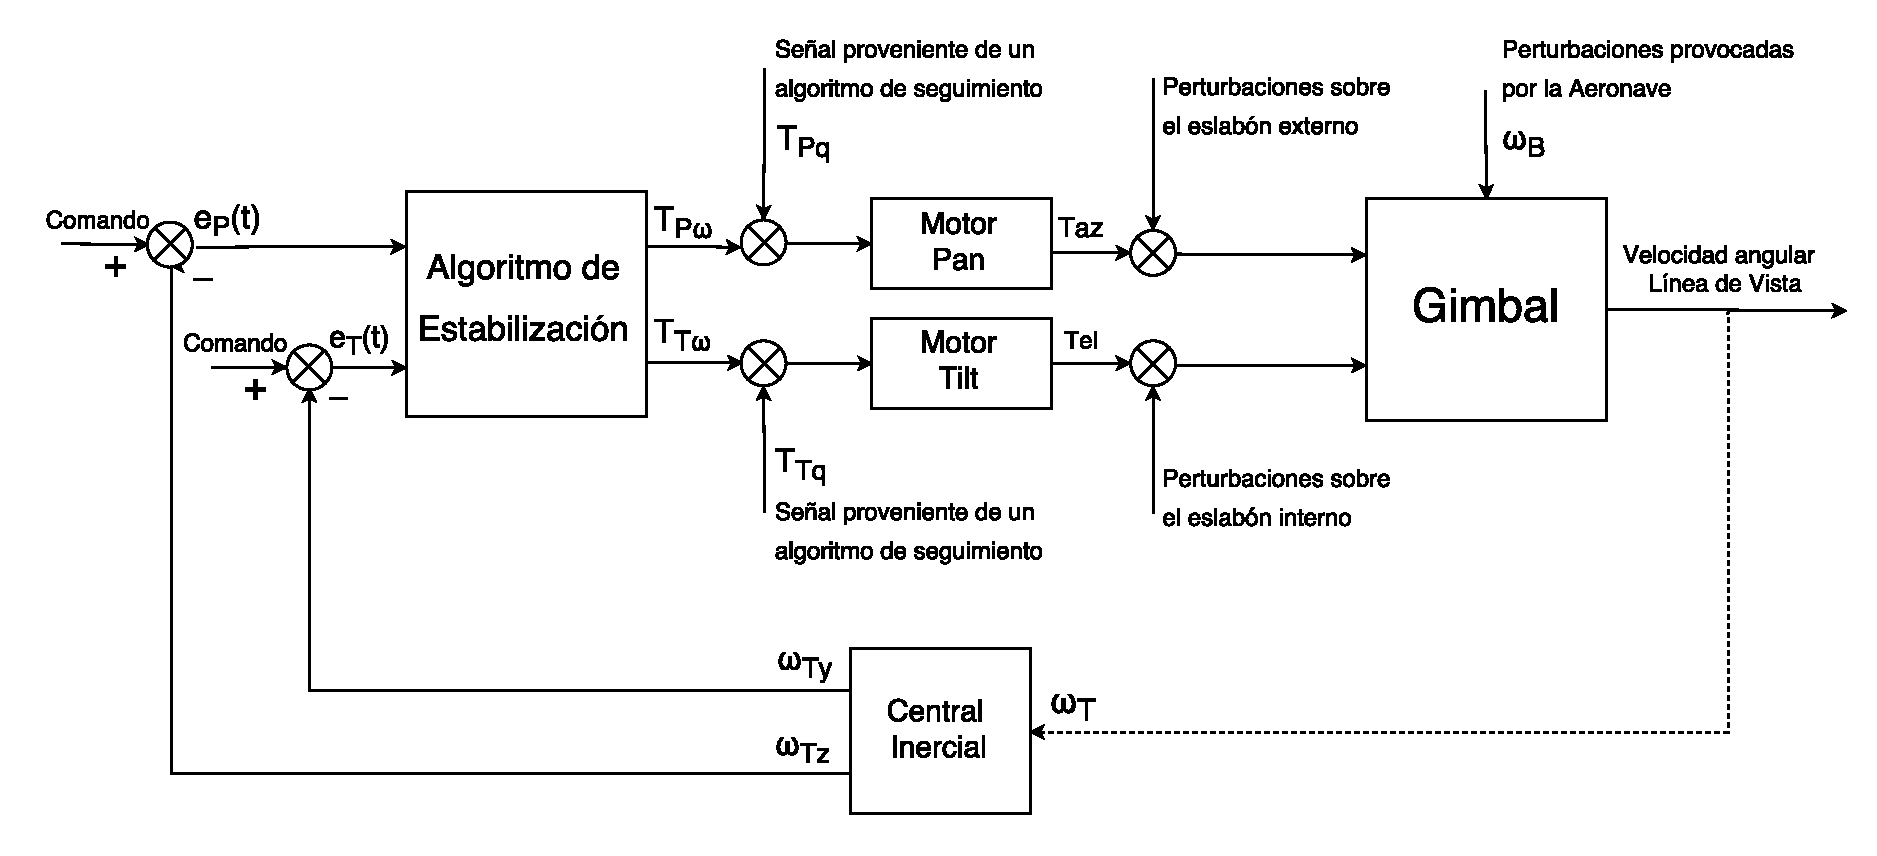
\includegraphics[scale=0.45]{img/DiagControl.pdf}
      \caption{Configuraci\'{o}n para el lazo de control de estabilizaci\'{o}n directa}
      \label{fig:BloquesCont}
\end{figure}

En la formulaci\'{o}n de cualquier problema de control siempre habr\'{a} una discrepancia entre la din\'{a}mica real del sistema y el modelo din\'{a}mico usado para dise\~{n}ar el controlador. Estas discrepancias surgen de perturbaciones externas desconocidas, par\'{a}metros de la planta, y din\'{a}micas no modeladas y parasitarias. Debido a esto se han desarrollado de m\'{e}todos de control robusto como un m\'{e}todo para compensar la inexactitud del modelado \cite{21}. Un enfoque simple del control robusto es la llamada metodolog\'{i}a de control de modos deslizantes. Intuitivamente, se basa en la observaci\'{o}n de que es mucho m\'{a}s f\'{a}cil controlar sistemas de primer orden, es decir sistemas descritos por ecuaciones diferenciales de primer orden ya sean no lineales o con incertidumbres en sus par\'{a}metros que controlar sistemas de orden \textit{n}, para lograr esto, se introduce una simplificaci\'{o}n notacional que permite reemplazar los sistemas de orden \textit{n} por problemas equivalentes de primer orden. Para los sistemas modificados, es posible probarse al menos en principio que se puede alcanzar un desempe\~{n}o \textit{"perfecto"}, en la presencia inexactitudes arbitrarias en los par\'{a}metros. Sin embargo, tal desempe\~{n} es obtenido con la consecuencia de una actividad extremadamente alta en la se\~{n}al de control (Chattering), este fen\'{o}meno es un efecto no deseado que puede generar inestabilidad en la din\'{a}mica del sistema al excitar din\'{a}micas internas no consideradas. 

En este cap\'{i}tulo se presenta el dise\~{n}o de un algoritmo de control por la metodolog\'{i}a de modos deslizantes y posteriormente se compara con un compensador PI frecuentemente usado para el control de este tipo de sistemas, con el fin de tener una referencia para medir el desempe\~{n}o del algoritmo dise\~{n}ado. Se realizan varias simulaciones elaborando un modelo en Simulink del modelo din\'{a}mico obtenido en las ecuaciones ~\ref{eq:Elev} y ~\ref{CrossEl} as\'{i} como de las leyes de control obtenidas.

 
\section{Control Sliding Mode} \label{sec:ControlSM}

El objetivo es controlar la velocidad angular sobre los ejes de elevaci\'{o}n y elevaci\'{o}n cruzada. Por consiguiente, las velocidades angulares $\omega _{T_y}$ y $\omega _{T_z}$ son las variables a controlar por el sistema de lazo cerrado. El prop\'{o}sito es mantener $\omega _{T_y}=\omega _{T_z}=0$ a pesar de las perturbaciones, y mantener sin rotaci\'{o}n el sensor con respecto al marco inercial. 

Las ecuaciones que describen el sistema gimbal bajo consideraci\'{o}n son altamente no lineales e incluyen t\'{e}rminos que no son conocidos con precisi\'{o}n o que no pueden ser medidos con precisi\'{o}n durante el vuelo. Se ha demostrado que el uso de control de estructura variable o control por modos deslizantes pueden proveer un desempe\~{n}o de seguimiento robusto en presencia de no linealidades e incertidumbres \cite{13}.


\subsection{Control de Elevaci\'{o}n}

En la secci\'{o}n ~\ref{sec:DinDes} se desarroll\'{o} la din\'{a}mica deseada para el canal de elevaci\'{o}n del sistema gimbal, la cual esta dada por la ecuaci\'{o}n ~\ref{eq:ElDinDes}. Esta ecuaci\'{o}n fue obtenida al considerar ciertas condiciones de simetr\'{i}a, bajo estas condiciones las perturbaciones inerciales desaparecen dejando \'{u}nicamente el par producido por el motor. 

Ahora para dise�ar el control podemos considerar las perturbaciones tales como la fricci\'{o}n, los pares debidos a masas no balanceadas, gradiente gravitacional, etc. como una sola perturbaci\'{o}n acotada, con lo anterior podemos reescribir la din\'{a}mica de elevaci\'{o}n como

\begin{equation}
I_{T_y}\dot{\omega}_{T_z} = T_{el} + f(x_{1_T},x_{2_T},t)
\label{eq:ContElevDina}
\end{equation}

Donde las variables de estado se definen de la siguiente manera

\begin{equation}
\begin{array}{c}
x_{1_T}=\int_0^t \! \omega _{T_y}(t) \,\mathrm{d}t \\ \\
\dot{x}_{1_T}=x_{2_T}=\omega _{T_y}
\end{array}
\label{eq:statevar}
\end{equation}

Y la funci\'{o}n $f(x_{1_T},x_{2_T},t)$ es el t\'{e}rmino de pertubaci\'{o}n el cual engloba todas las no linealidades de la ecuaci\'{o}n ~\ref{Elev_2} as\'{i} como cualquier otra perturbaci\'{o}n no considerada en el modelado. Se asume que esta funci\'{o}n esta acotada de tal manera que $\abs{f(x_{1_T},x_{2_T},t)} \leq L > 0$ y esta dada por

\begin{equation}
\begin{array}{cl}
f(x_{1_T},x_{2_T},t) = & -k_{Tvf} \, \omega_{T_y} + \left[ t\varepsilon \, \left(I_{T_x}-I_{T_z}\right) \right]\omega_{T_y}^2 + \\
 &\left[ \frac{1}{c \varepsilon} \left(I_{T_z}-I_{T_x}\right) \right] \left[ c \eta \omega_{B_x} \omega _{T_z} + s \eta \omega_{B_y} \omega _{T_z} \right] + k_{Tvf} \, \left[ c \eta \omega_{B_y} - s \eta \omega_{B_x} \right] \\
 & -  k_{Tcf} \, \mathrm{sign}\left( \omega_{T_y} - c \eta \omega_{B_y} + s \eta \omega_{B_x} \right) + T_{U_{Ty}}
\end{array}
\label{eq:fxT}
\end{equation}

Ahora usando las definiciones de las variables de estado dadas en ~\ref{eq:statevar}, podemos transformar la ecuaci\'{o}n ~\ref{eq:ContElevDina} en su representaci\'{o}n en variables de estado

\begin{equation}
\dot{x}_{2_T}=\frac{1}{I_{T_y}}T_{el} + f(x_{1_T},x_{2_T},t)
\end{equation}

Si elegimos $T_{el}=I_{T_y}u_T$ donde $u_T$ es una entrada de control equivalente, la din\'{a}mica resultante es

\begin{equation}
\overset{.}{x}_{2_T}= u_T + f(x_{1_T},x_{2_T},t)
\end{equation}

Ahora definimos la superficie de deslizamiento, como

\begin{equation}
\sigma_{T}=c_{T}x_{1_T} + x_{2_T}, \, c>0
\end{equation}

A fin de lograr la convergencia asint\'{o}tica de las variables de estado $x_{1_T}$, $x_{2_T}$ en la presencia de la perturbaci\'{o}n acotada $f(x_{1_T},x_{2_T},t)$, aplicaremos Lyapunov a la din\'{a}mica de $\sigma_{T}$, derivando obtenemos

\begin{equation}
\dot{\sigma}_{T}=c_{T}x_{2_T}+ f(x_{1_T},x_{2_T},t)+u_T,\, \sigma_{T}(0)=0
\label{eq:sigma_dot}
\end{equation}


La siguiente funci\'{o}n candidata de Lyapunov se elije para probar la estabilizaci\'{o}n de la din\'{a}mica de $\sigma$

\begin{equation}
\mathrm{V}=\frac{1}{2}\sigma_{T}^2
\end{equation}

A fin de proporcionar estabilidad asint\'{o}tica de ~\ref{eq:sigma_dot} alrededor del punto de equilibrio $\sigma_{T}=0$, las siguientes condiciones deben satisfacerse 

\begin{enumerate}[a)]
 \item{$\dot{\mathrm{V}}<0$ para $\sigma_{T} \neq 0$}
 \item{$\lim_{\abs{\sigma_{T}} \to \infty }\mathrm{V}= \infty$}
\end{enumerate}


La condici\'{o}n (b) obviamente, se satisface con $\mathrm{V}$. A fin de lograr la convergencia en tiempo finito, la condici\'{o}n (a) puede ser modificada para ser 

\begin{equation}
\dot{\mathrm{V}} \leq - \alpha \mathrm{V}^{1/2}, \, \alpha < 0
\end{equation}


Calculando la derivada de $\mathrm{V}$, obtenemos

\begin{equation}
\overset{.}{\mathrm{V}}=\overset{.}{\sigma_{T}}\sigma_{T} = \sigma_{T} \left( c_{T}x_{2_T} + f(x_{1_T},x_{2_T},t) + u_T \right)
\end{equation}


Asumiendo que $u_T=-c_{T}x_{2_T}+v$ y sustituyendo en la expresi\'{o}n anterior, obtenemos

\begin{equation}
\begin{array}{cl}
\dot{\mathrm{V}}= & \sigma_{T} \left( f(x_{1_T},x_{2_T},t)+ v \right) \\
                  & \sigma_{T} f(x_{1_T},x_{2_T},t) + \sigma_{T} v \leq \abs{\sigma_{T}} L + \sigma_{T} v
\end{array}
\label{eq:V_dot}
\end{equation}

Eligiendo $v=-\rho_{T} \, \mathrm{sign} \left( \sigma_{T} \right)$, donde

\begin{equation}
\mathrm{sign}(x) = \begin{cases} 1 &\mbox{if } x > 0 \\
 0 &\mbox{if } x = 0 \\
-1 & \mbox{if } x < 0. \end{cases}
\end{equation}

Con $\rho_{T} > 0$ y substituyendo en ~\ref{eq:V_dot}, obtenemos

\begin{equation}
\dot{\mathrm{V}} \leq \abs{\sigma_{T}}L - \rho_{T} \abs{\sigma_{T}} = -\abs{\sigma_{T}} \left( \rho_{T} -L \right)
\label{eq:V_dot_2}
\end{equation}

Podemos ver de ~\ref{eq:V_dot_2} que mientras $\rho_{T} > L$ la estabilidad esta garantizada. Por lo tanto, finalmente la ley de control para el canal de elevaci\'{o}n es

\begin{equation}
T_{el}=I_{T_y} \left( -c_{T}\omega_{T_y} - \rho_{T} \, \mathrm{sign} \left( \sigma_{T} \right) \right)
\label{eq:ElevControlSM}
\end{equation}


\subsection{Control de Elevaci\'{o}n Cruzada}

Al igual que con la din\'{a}mica de elevaci\'{o}n, consideraremos a las perturbaciones inerciales, el par causado por la fricci\'{o}n, y las din\'{a}micas no modeladas, como una sola perturbaci\'{o}n acotada $f(x_{1_P},x_{2_P},t)$, reescribiendo la ecuaci\'{o}n ~\ref{CrossEl}, tenemos

\begin{equation}
Js\dot{\omega}_{T_z} = c\varepsilon T_{az} + f(x_{1_P},x_{2_P},t)
\end{equation}

donde

\begin{equation}
\begin{array}{c}
x_{1_P}=\int_0^t \! \omega _{T_z}(t) \,\mathrm{d}t \\ \\
\dot{x}_{1_P}=x_{2_P}=\omega _{T_z}
\end{array}
\label{eq:statevarAz}
\end{equation}

Son las variables de estado y la funci\'{o}n $f(x_{1_P},x_{2_P},t)$ es el t\'{e}rmino de pertubaci\'{o}n el cual engloba todas las no linealidades de la ecuaci\'{o}n ~\ref{CrossEl} as\'{i} como cualquier otra perturbaci\'{o}n no considerada en el modelado. Se asume que esta funci\'{o}n esta acotada de tal manera que $\abs{f(x_{1_P},x_{2_P},t)} \leq L_P > 0$.

Siguiendo el mismo proceso que para el dise\~{n}o del control de elevaci\'{o}n, obtenemos la ley de control para el canal de acimut o elevaci\'{o}n cruzada, dado por

\begin{equation}
T_{az}=\frac{Js}{c\varepsilon} \left( -c_{P}\omega_{T_z} - \rho_{P} \, \mathrm{sign} \left( \sigma_{P} \right) \right)
\end{equation}


\subsection{Reducci\'{o}n del Efecto "Chattering"} \label{sec:ChatRed}

En los sistemas de control de motores CD, es importante evitar el effecto de casta\~{n}eo o \textit{"chattering"} al proveer se�ales de control continuas y suaves. Una soluci\'{o}n para lograr esto, es aproximar la funci\'{o}n discontinua $\mathrm{sign}(x)$ a alguna alternativa continua. Por ejemplo, puede ser reemplazada por una funci\'{o}n sigmoide\cite{21}, dada por

\begin{equation}
\mathrm{sign}(x) \approx \frac{x}{\abs{x}+\epsilon}
\label{eq:sigmoide}
\end{equation}

Donde $\epsilon$ es un escalar peque\~{n}o y positivo, tal que

\begin{equation}
\lim_{\epsilon \to 0}\frac{x}{\abs{x}+\epsilon}=\mathrm{sign}(x); \, x \neq 0
\end{equation}


\section{Compensador Proporcional-Integral}

Tal como se menciona en \cite{6}, el controlador PID convencional y sus constructores (P, PI y PD) son los algoritmos m\'{a}s utilizados debido a su estructura simple, bajo costo, dise�o simple y alto desempe\~{n}o, siendo el compensador proporcional-integral (PI) un algoritmo frecuentemente utilizado para el control de sistemas de estabilizaci\'{o}n inercial \cite{3}. Es por este motivo que este m\'{e}todo de control se utilizar\'{a} como un punto de referencia para medir el desempe\~{n}o del algoritmo de control robusto dise\~{n}ado en la secci\'{o}n anterior ~\ref{sec:ControlSM}. Las ecuaciones del compensador proporcional-integral para el canal de elevaci\'{o}n y elevaci\'{o}n cruzada se muestran en ~\ref{eq:ContPIElev} y ~\ref{eq:ContPICross} respectivamente.

\begin{equation}
T_{el}=-\left(K_{P_{el}}\omega_{T_y}+ K_{I_{el}} \int_{0}^{t} \! \omega _{T_y}(\tau) \,\mathrm{d}\tau  \right)
\label{eq:ContPIElev}
\end{equation}

\begin{equation}
T_{az}=-\left(K_{P_{az}}\omega_{T_z}+ K_{I_{az}} \int_{0}^{t} \! \omega _{T_z}(\tau) \,\mathrm{d}\tau  \right)
\label{eq:ContPICross}
\end{equation}
\newpage

\section{Simulaciones}

El modelo desarrollado en la secci\'{o}n ~\ref{sec:Modelado}, definido por la ecuaciones ~\ref{Elev_2} y ~\ref{CrossEl}, se construye en el entorno de simulaci\'{o}n Simulink\textsuperscript{\textregistered} de MATLAB\textsuperscript{\textregistered}, figura~\ref{fig:GimbalSimulink}, con el prop\'{o}sito de obtener una comparaci\'{o}n cuantitativa entre el algoritmo de estabilizaci\'{o}n por modos deslizantes dise\~{n}ado en este cap\'{i}tulo y un compensador proporcional-integral com\'{u}nmente usado para estos sistemas. Para la obtenci\'{o}n de los par\'{a}metros inerciales del sistema se realiz\'{o} un modelo detallado en 3D empleando el programa SolidWorks\textsuperscript{\textregistered}, con esta herramienta fue posible obtener una aproximaci\'{o}n del valor de la matriz de inercia necesaria para la simulaci\'{o}n. Los par\'{a}metros inerciales para el eslab\'{o}n interno y externo se muestran en la tabla ~\ref{Table:IGparameters}. 

\begin{figure}[H]
      \centering
      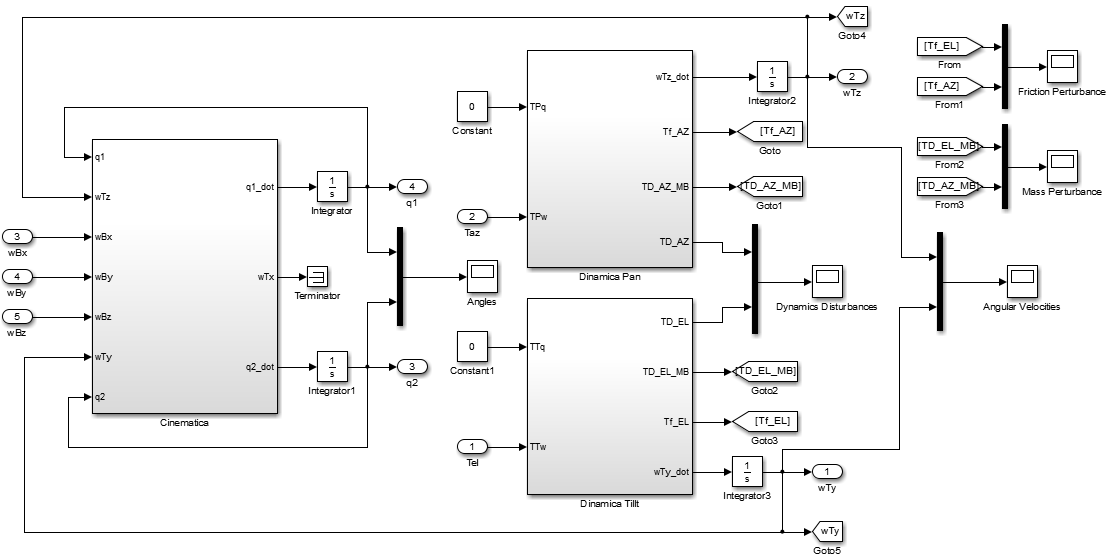
\includegraphics[scale=0.5]{Img/GimbalSimulink.png}
      \caption{Simulation Block Diagram}
      \label{fig:GimbalSimulink}
\end{figure}

\begin{table}[H]
\caption{Par\'{a}metros Inerciales del Eslab\'{o}n Interno}
\label{Table:IGparameters}
\begin{center}
\begin{tabular}{ |c|c| }
\hline
\multicolumn{2}{ |c| }{\textbf{Par\'{a}metros Inerciales Eslab\'{o}n Interno}} \\
\hline
\textit{Variable} & \textit{Valor} \\
\hline
$I_{T_x}$ & $1.68\e{-4} \left(kg \cdot m^2\right)$  \\
$I_{T_y}$ & $1.78\e{-4} \left(kg \cdot m^2\right)$  \\
$I_{T_z}$ & $1.16\e{-4} \left(kg \cdot m^2\right)$  \\
 \hline
 \multicolumn{2}{ |c| }{\textbf{Par\'{a}metros Inerciales Eslab\'{o}n Externo}} \\
\hline
\textit{Variable} & \textit{Valor} \\
\hline
$I_{P_x}$ & $2.62\e{-3} \left(kg \cdot m^2\right)$  \\
$I_{P_y}$ & $2.47\e{-3} \left(kg \cdot m^2\right)$  \\
$I_{P_z}$ & $4.66\e{-4} \left(kg \cdot m^2\right)$  \\
\hline
\end{tabular}
\end{center}
\end{table}

Como se detalla en la secci\'{o}n ~\ref{sec:Implementacion} en el prototipo se utilizan baleros tipo bola de alta precision para la construcci\'{o}n del gimbal, lo cual permite reducir el efecto de la fricci\'{o}n al m\'{i}nimo,  Los par\'{a}metros de los coeficientes de fricci\'{o}n para la simulaci\'{o}n se obtienen de la literatura \cite{3}, \cite{24} y se muestran en la tabla ~\ref{Table:FrictionParameters} 

\begin{table}[H]
\caption{Coeficientes de Fricci\'{o}n}
\label{Table:FrictionParameters}
\begin{center}
\begin{tabular}{ |c|c| }
\hline
 \multicolumn{2}{ |c| }{\textbf{Coeficientes de Fricci\'{o}n para el Eslab\'{o}n Interno y Externo}} \\
\hline
\textit{Variable} & \textit{Valor} \\
\hline
$k_{Tvf}$, $k_{Pvf}$ & $5.2\e{-3} \left(N \cdot m/rad/s\right)$  \\
$k_{Tcf}$, $k_{Pcf}$ & $3.6\e{-3} \left(unit-less\right)$  \\
\hline
\end{tabular}
\end{center}
\end{table}

En la tabla~\ref{table:Bparameters} se muestran las se�ales de perturbaci\'{o}n empleadas para la simulaci\'{o}n del sistema de control, estas se\~{n}ales sinusoidales se emplean en todas las simulaciones para tener uniformidad al probar los algoritmos de control propuestos. Estas se�ales simulan las posibles velocidades angulares que el aeronave experimentar\'{i}a en roll pitch y yaw durante el vuelo. En la figura ~\ref{fig:PerturbacionesBase} se muestran las gr\'{a}ficas correspondientes a estas se\~{n}ales. 


\begin{table}[H]
\caption{Se�ales de Perturbaci\'{o}n al Sistema}
\label{table:Bparameters}
\begin{center}
\begin{tabular}{ |c|c|c| }
\hline
\multicolumn{3}{ |c| }{\textbf{Se\~{n}ales de Perturbaci\'{o}n}} \\
\hline
\textit{Variable} & \textit{Amplitud} & \textit{Frecuencia} \\
\hline
$\omega _{Bx}$ & $1.5 \left(rad/seg\right)$ & $0.1 \left(Hz\right)$ \\
$\omega _{By}$ & $0.2 \left(rad/seg\right)$ & $0.3 \left(Hz\right)$  \\
$\omega _{Bz}$ & $0.8 \left(rad/seg\right)$ & $1 \left(Hz\right)$  \\
 \hline
\end{tabular}
\end{center}
\end{table}

\begin{figure}[H]
      \centering
      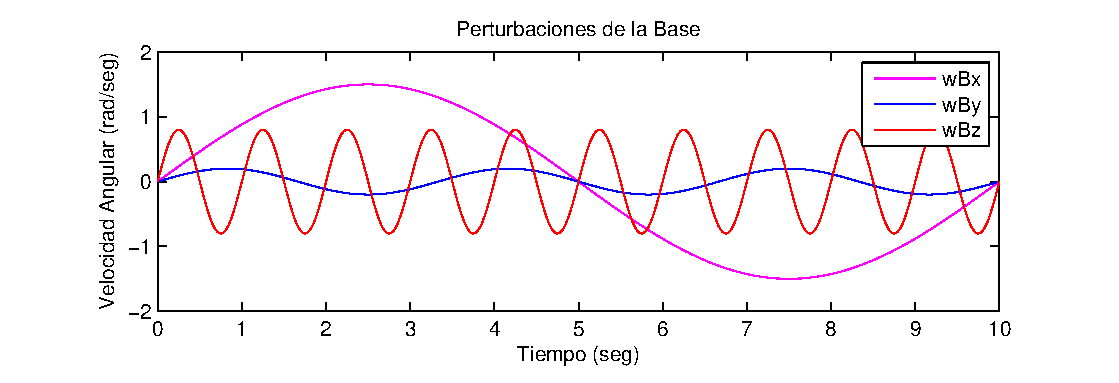
\includegraphics[scale=0.9]{Img/BasePerturbance.eps}
      \caption{Perturbaciones de la Base}
      \label{fig:PerturbacionesBase}
\end{figure} 

En la figura ~\ref{fig:ChatRed}-a podemos observar los cambios de alta frecuencia y amplitud finita propios del control por modos deslizantes, estos cambios se presentan cuando el sistema alcanza la superficie de deslizamiento y es un efecto no deseado en el control de motores DC, adem\'{a}s de que el ata actividad del control puede excitar din\'{a}micas parasitarias en el sistema. Para evitar este efecto, se emplea una funci\'{o}n sigmoide tal como se detalla en la secci\'{o}n ~\ref{sec:ChatRed}. En la figura ~\ref{fig:ChatRed}-b podemos observar la reducci\'{o}n del efecto chattering gracias al uso de la funci\'{o}n sigmoide ~\ref{eq:sigmoide} con un valor de $\epsilon=0.001$.

\begin{figure}[H]
      \centering
      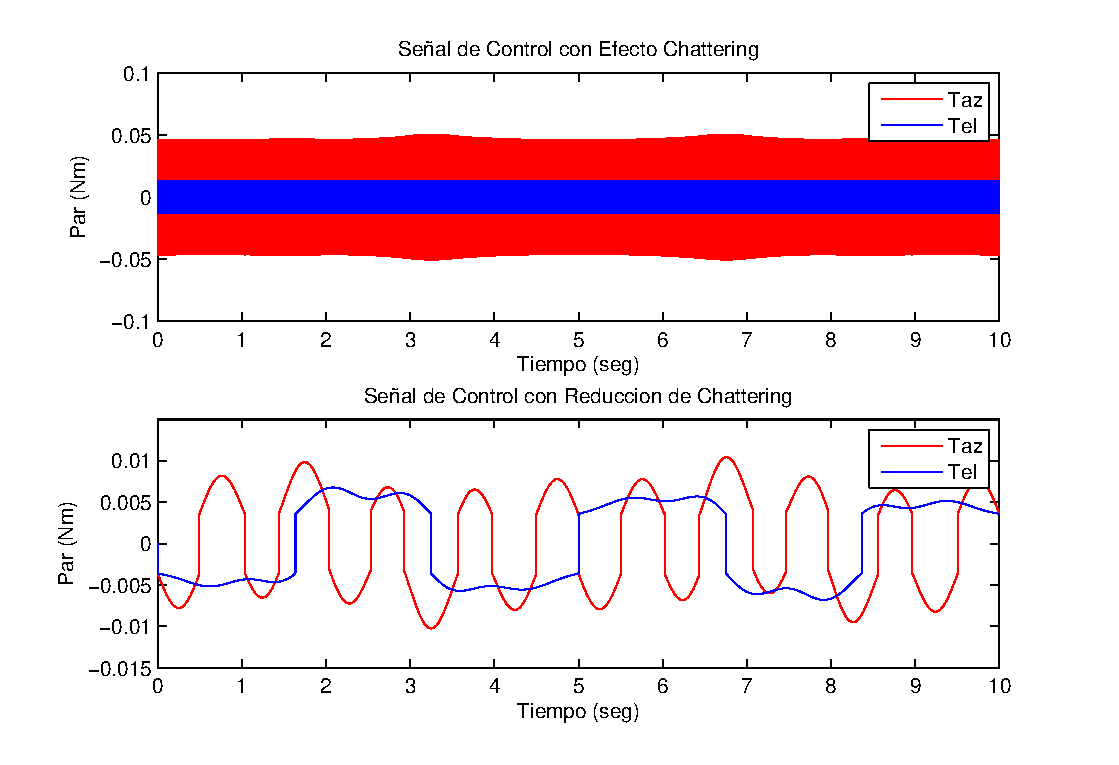
\includegraphics[scale=0.9]{img/ChatteringRed.eps}
      \caption{Reducci\'{o}n del Efecto Chattering}
      \label{fig:ChatRed}
\end{figure} 

En la figura ~\ref{fig:ContrAcc} podemos apreciar una comparaci\'{o}n entre la ley de control por modos deslizantes con dise\~{n}ada y el compensador proporcional-integral, esta comparaci\'{o}n se realiza debido a que como se ha mencionado anteriormente, los controladores PID y sus constructores siguen siendo muy utilizados debido a su simple dise\~{n}o , alto desempe\~{n}o y bajo costo, siendo el compensador PI frecuentemente utilizado para el control de este tipo de sistemas \cite{3}. La figura ~\ref{fig:ContrAcc}-a muestra la respuesta del sistema al control por modos deslizantes dise\~{n}ado, mientras que en en la figura ~\ref{fig:ContrAcc}-b se muestra la respuesta al compensador PI, podemos observar que ambos controles tienen un buen desempe\~{n}o ya que ambos son capaces de cancelar las perturbaciones del movimiento de la base, sin embargo podemos observar que el algoritmo dise\~{n}ado tiene un mejor desempe\'{n}o en la convergencia de las variables controladas $\omega _{T_y}$ y $\omega _{T_z}$.

\begin{figure}[H]
      \centering
      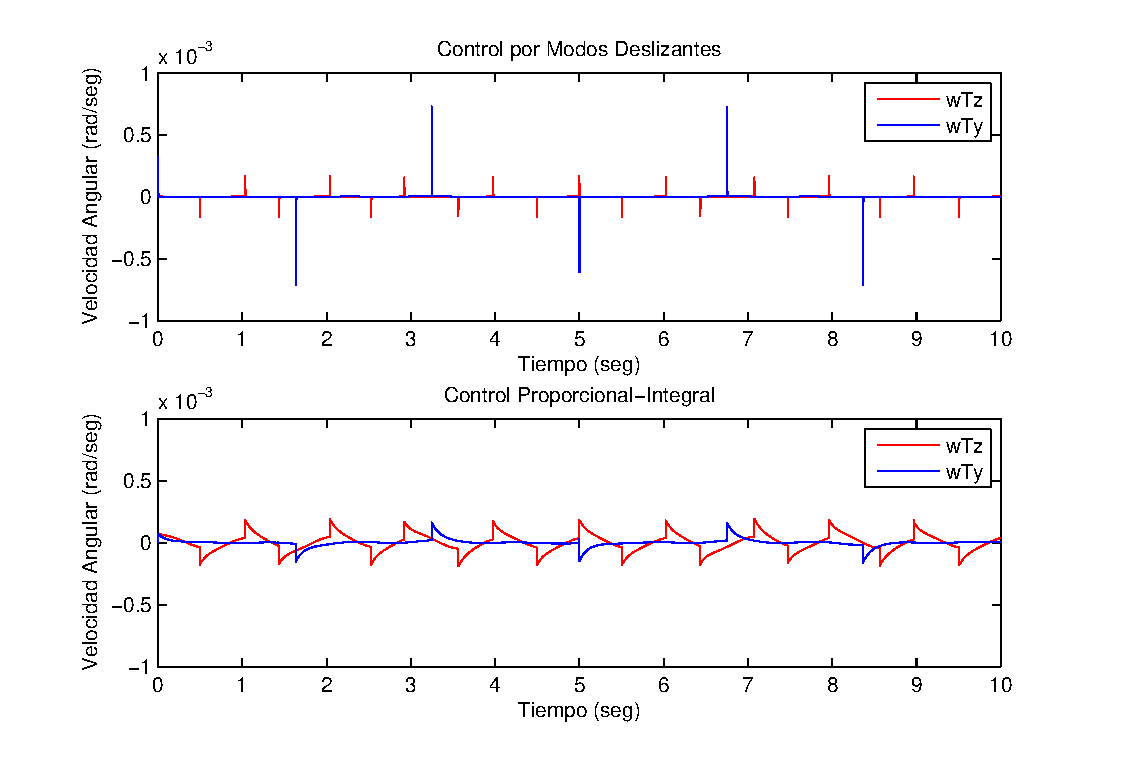
\includegraphics[scale=0.9]{img/VelAngular.eps}
      \caption{Acci\'{o}n de Control del Algoritmo de Modos Deslizantes vs Compensador PI}
      \label{fig:ContrAcc}
\end{figure}

La figura ~\ref{fig:SenalCont} muestra las se\~{n}ales de control del algoritmo por modos deslizantes y el compensador PI. Las se\~{n}ales de control del control por modos deslizantes de muestra en la figura ~\ref{fig:SenalCont}-a, mientras que la se\~{n}al de control del compensador PI se muestra en la figura ~\ref{fig:SenalCont}-b, Ambas se\~{n}ales son muy similares, pero las peque\~{n}as diferencias afectan la respuesta del sistema como muestra la figura ~\ref{fig:ContrAcc}. La se\~{n}al de control intenta cancelar las perturbaciones de la base del sistema, con el fin de mantener las variables controladas $\omega _{T_y}$ y $\omega _{T_z}$ iguales a cero, una de las perturbaciones que m\'{a}s afectan el desempe\~{n}o del sistema es el par provocado por la fricci\'{o}n tal como se menciona en \cite{10} especialmente durante los cambios de direcci\'{o}n del eslab\'{o}n interno y externo, siendo una de las influencias clave en la forma de onda de la se\~{n}al de control.  

\begin{figure}[H]
      \centering
      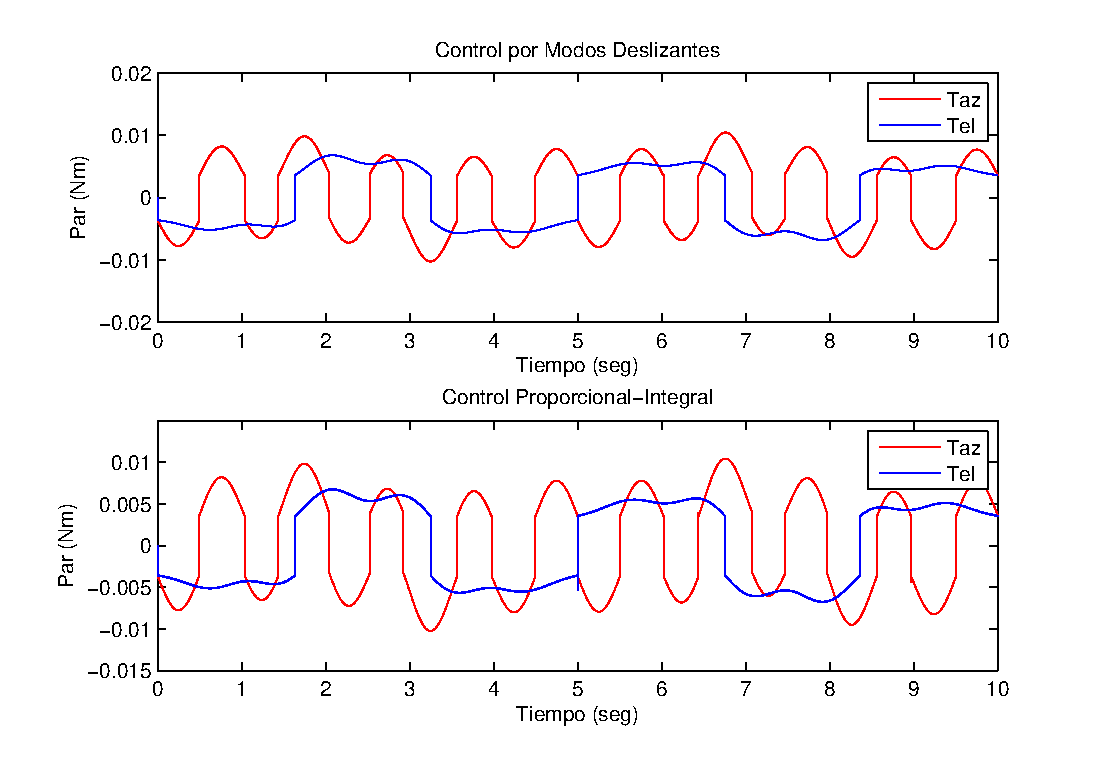
\includegraphics[scale=0.9]{img/SenalCont.eps}
      \caption{Se\~{a}l de Control del Algoritmo de Modos Deslizantes vs Compensador PI}
      \label{fig:SenalCont}
\end{figure}

Para una mejor idea de la efectividad del control dise\~{n}ado en la cancelaci\'{o}n de las perturbaciones provocadas por el movimiento del aeronave se realiza una simulaci\'{o}n en la que los primeros segundos no se aplica alg\'{u}n control y posteriormente, exactamente a los tres segundos se activa el control. En la figura ~\ref{fig:ControlEffect}-a se muestran las perturbaciones a las que esta expuesto el sistema. En la figura ~\ref{fig:ControlEffect}-b muestra las variables controladas $\omega _{T_y}$ y $\omega _{T_z}$. Podemos observar que cuando el control es activado estas r\'{a}pidamente convergen a cero y se logra la cancelaci\'{o}n de las perturbaciones de la base. Finalmente en la figura ~\ref{fig:ControlEffect}-c se muestra la variaci\'{o}n en los \'{a}ngulos del eslab\'{o}n interno y el externo para compensar el movimiento de la base.      


\begin{figure}[H]
      \centering
      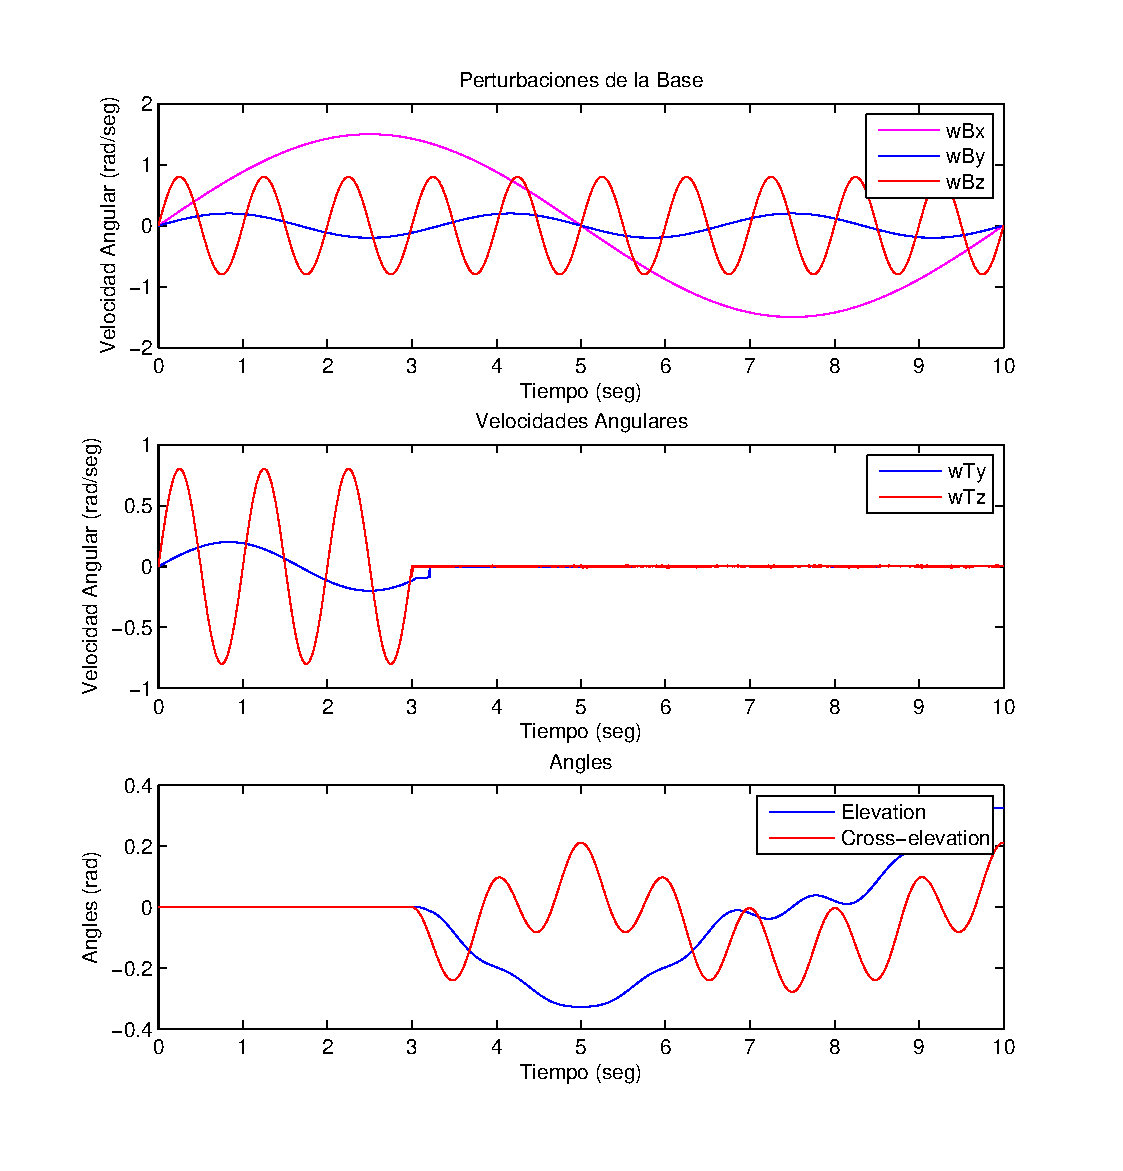
\includegraphics[scale=0.9]{img/ControlEffect.eps}
      \caption{Respuesta del Sistema al Aplicarse el Algoritmo de Estabilizaci\'{o}n}
      \label{fig:ControlEffect}
\end{figure} %Control

\chapter{Implementaci\'on}\label{sec:Implementacion}

\section{Introducci\'on}

En este cap\'{i}tulo se detalla la construcci\'{o}n y estructura del prototipo desarrollado, En las figuras ~\ref{fig:GimbalModel} y ~\ref{fig:GimbalViews}, podemos observar el dise\~{n}o 3D del prototipo realizado en el programa de modelado y simulaci\'{o}n mec\'{a}nica SolidWorks\textsuperscript{\textregistered}, mientras que en la fotograf\'{i}a de la figura ~\ref{fig:PrototipoTerminado} observamos el prototipo terminado. Este prototipo se realiz\'{o} en conjunto con el Instituto de Investagaci\'{o}n y Desarrollo Tecnol\'{o}gico de la Armada de M\'{e}xico (INIDETAM) durante una estancia de seis meses en las instalaciones del instituto. La construcci\'{o}n del prototipo se divide en tres aspectos claves, la mec\'{a}nica, la electr\'{o}nica y la programaci\'{o}n. La mec\'{a}nica y electr\'{o}nica del prototipo se basa en el desarrollo realizado por el INIDETAM  previo al inicio de este trabajo. El desarrollo previo al inicio de la tesis consiste en el dise\~{n}o mec\'{a}nico b\'{a}sico del sistema, la estructura de soporte y montaje, el tipo y m\'{e}todo de transmisi\'{o}n de potencia de los motores a los eslabones interno y externo del sistema, la selecci\'{o}n del material as\'{i} como el maquinado. Por el lado del desarrollo electr\'{o}nico, en el instituto se dise\~{n}aron dos tarjetas electr\'{o}nicas dedicadas para el control del sistema, una para el control del movimiento de pan y el otro para el movimiento en tilt estas tarjetas cuentan con todos los dispositivos necesarios para el procesamiento y comunicaci\'{o}n del sistema, as\'{i} como para el control de los motores y la c\'{a}mara. Para la detecci\'{o}n de l\'{i}mites f\'{i}sicos del sistema, en el instituto se desarrollaron sensores de l\'{i}mite magn\'{e}ticos, los cuales no funcionaron en la implementaci\'{o}n por lo que tuvieron que ser redise\~{n}ados.          

\begin{figure}[H]
\centering 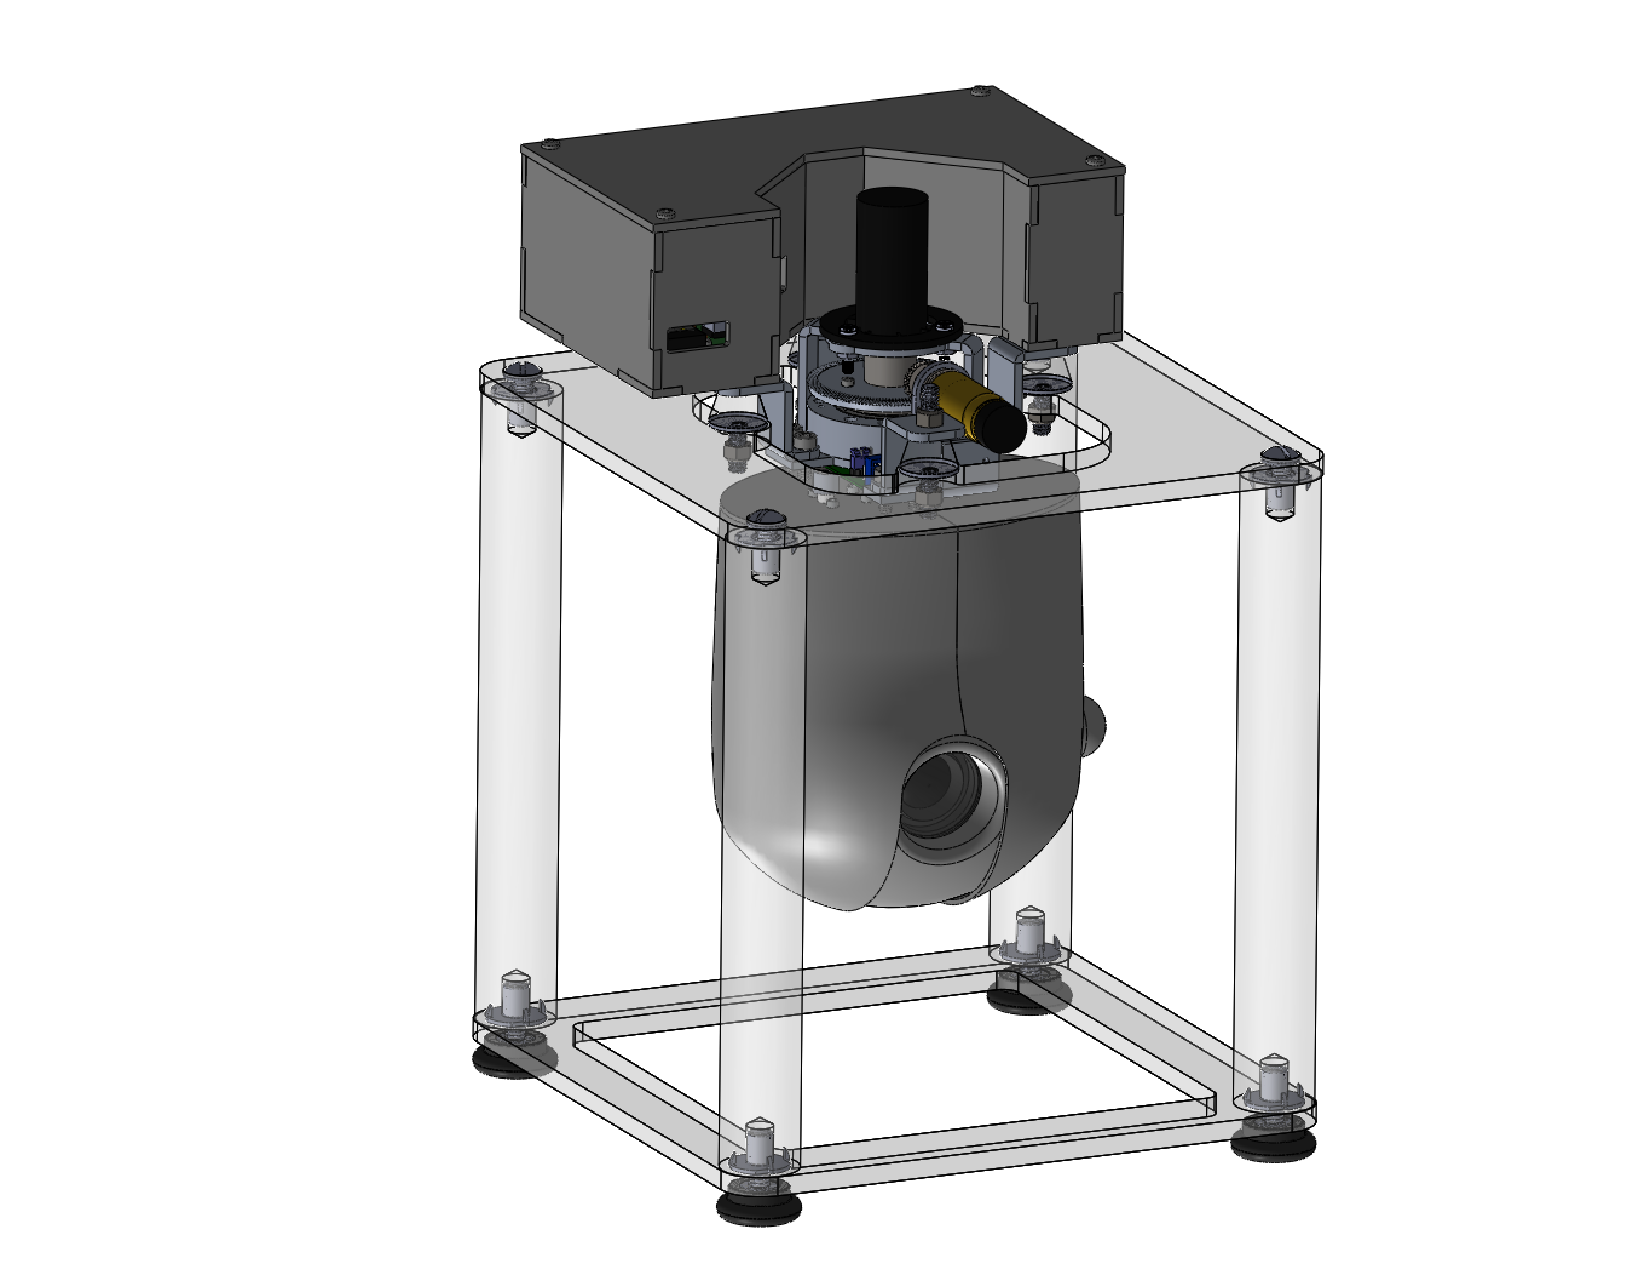
\includegraphics[scale=0.45]{img/Gimbal2.pdf}
%trim = izquierda abajo derecha arriba [scale=0.5,trim = 40mm 30mm 110mm 15mm, clip]
\caption{Modelo 3D del Prototipo de C\'{a}mara Giroestablizada}
\label{fig:GimbalModel}
\end{figure}

La programaci\'{o}n del microcontrolador se realiz\'{o} utilizando los MPLAB\textsuperscript{\textregistered} Device Blocks for Simulink\textsuperscript{\textregistered}. Esta herramienta creada por la empresa Microchip\textsuperscript{\textregistered}, permite utilizar el entorno de Simulink\textsuperscript{\textregistered} para la programaci\'{o}n de los microcontroladores Microchip\textsuperscript{\textregistered} de las familias dsPIC\textsuperscript{\textregistered}30 y dsPIC\textsuperscript{\textregistered}33. Esta herramienta permite la configuraci\'{o}n de los perif\'{e}ricos del microcontrolador a trav\'{e}s de bloques de Simulink, lo cual facilita en gran medida las aplicaciones. Tambi\'{e}n es posible a\~{n}adir bloques que ejecuten c\'{o}digo en lenguaje C, brindando la oportunidad que crear funciones personalizadas y tener acceso a caracter\'{i}sticas de los dsPIC\textsuperscript{\textregistered} no disponibles con los bloques predeterminados incluidos.  


\begin{figure}[H]
\centering 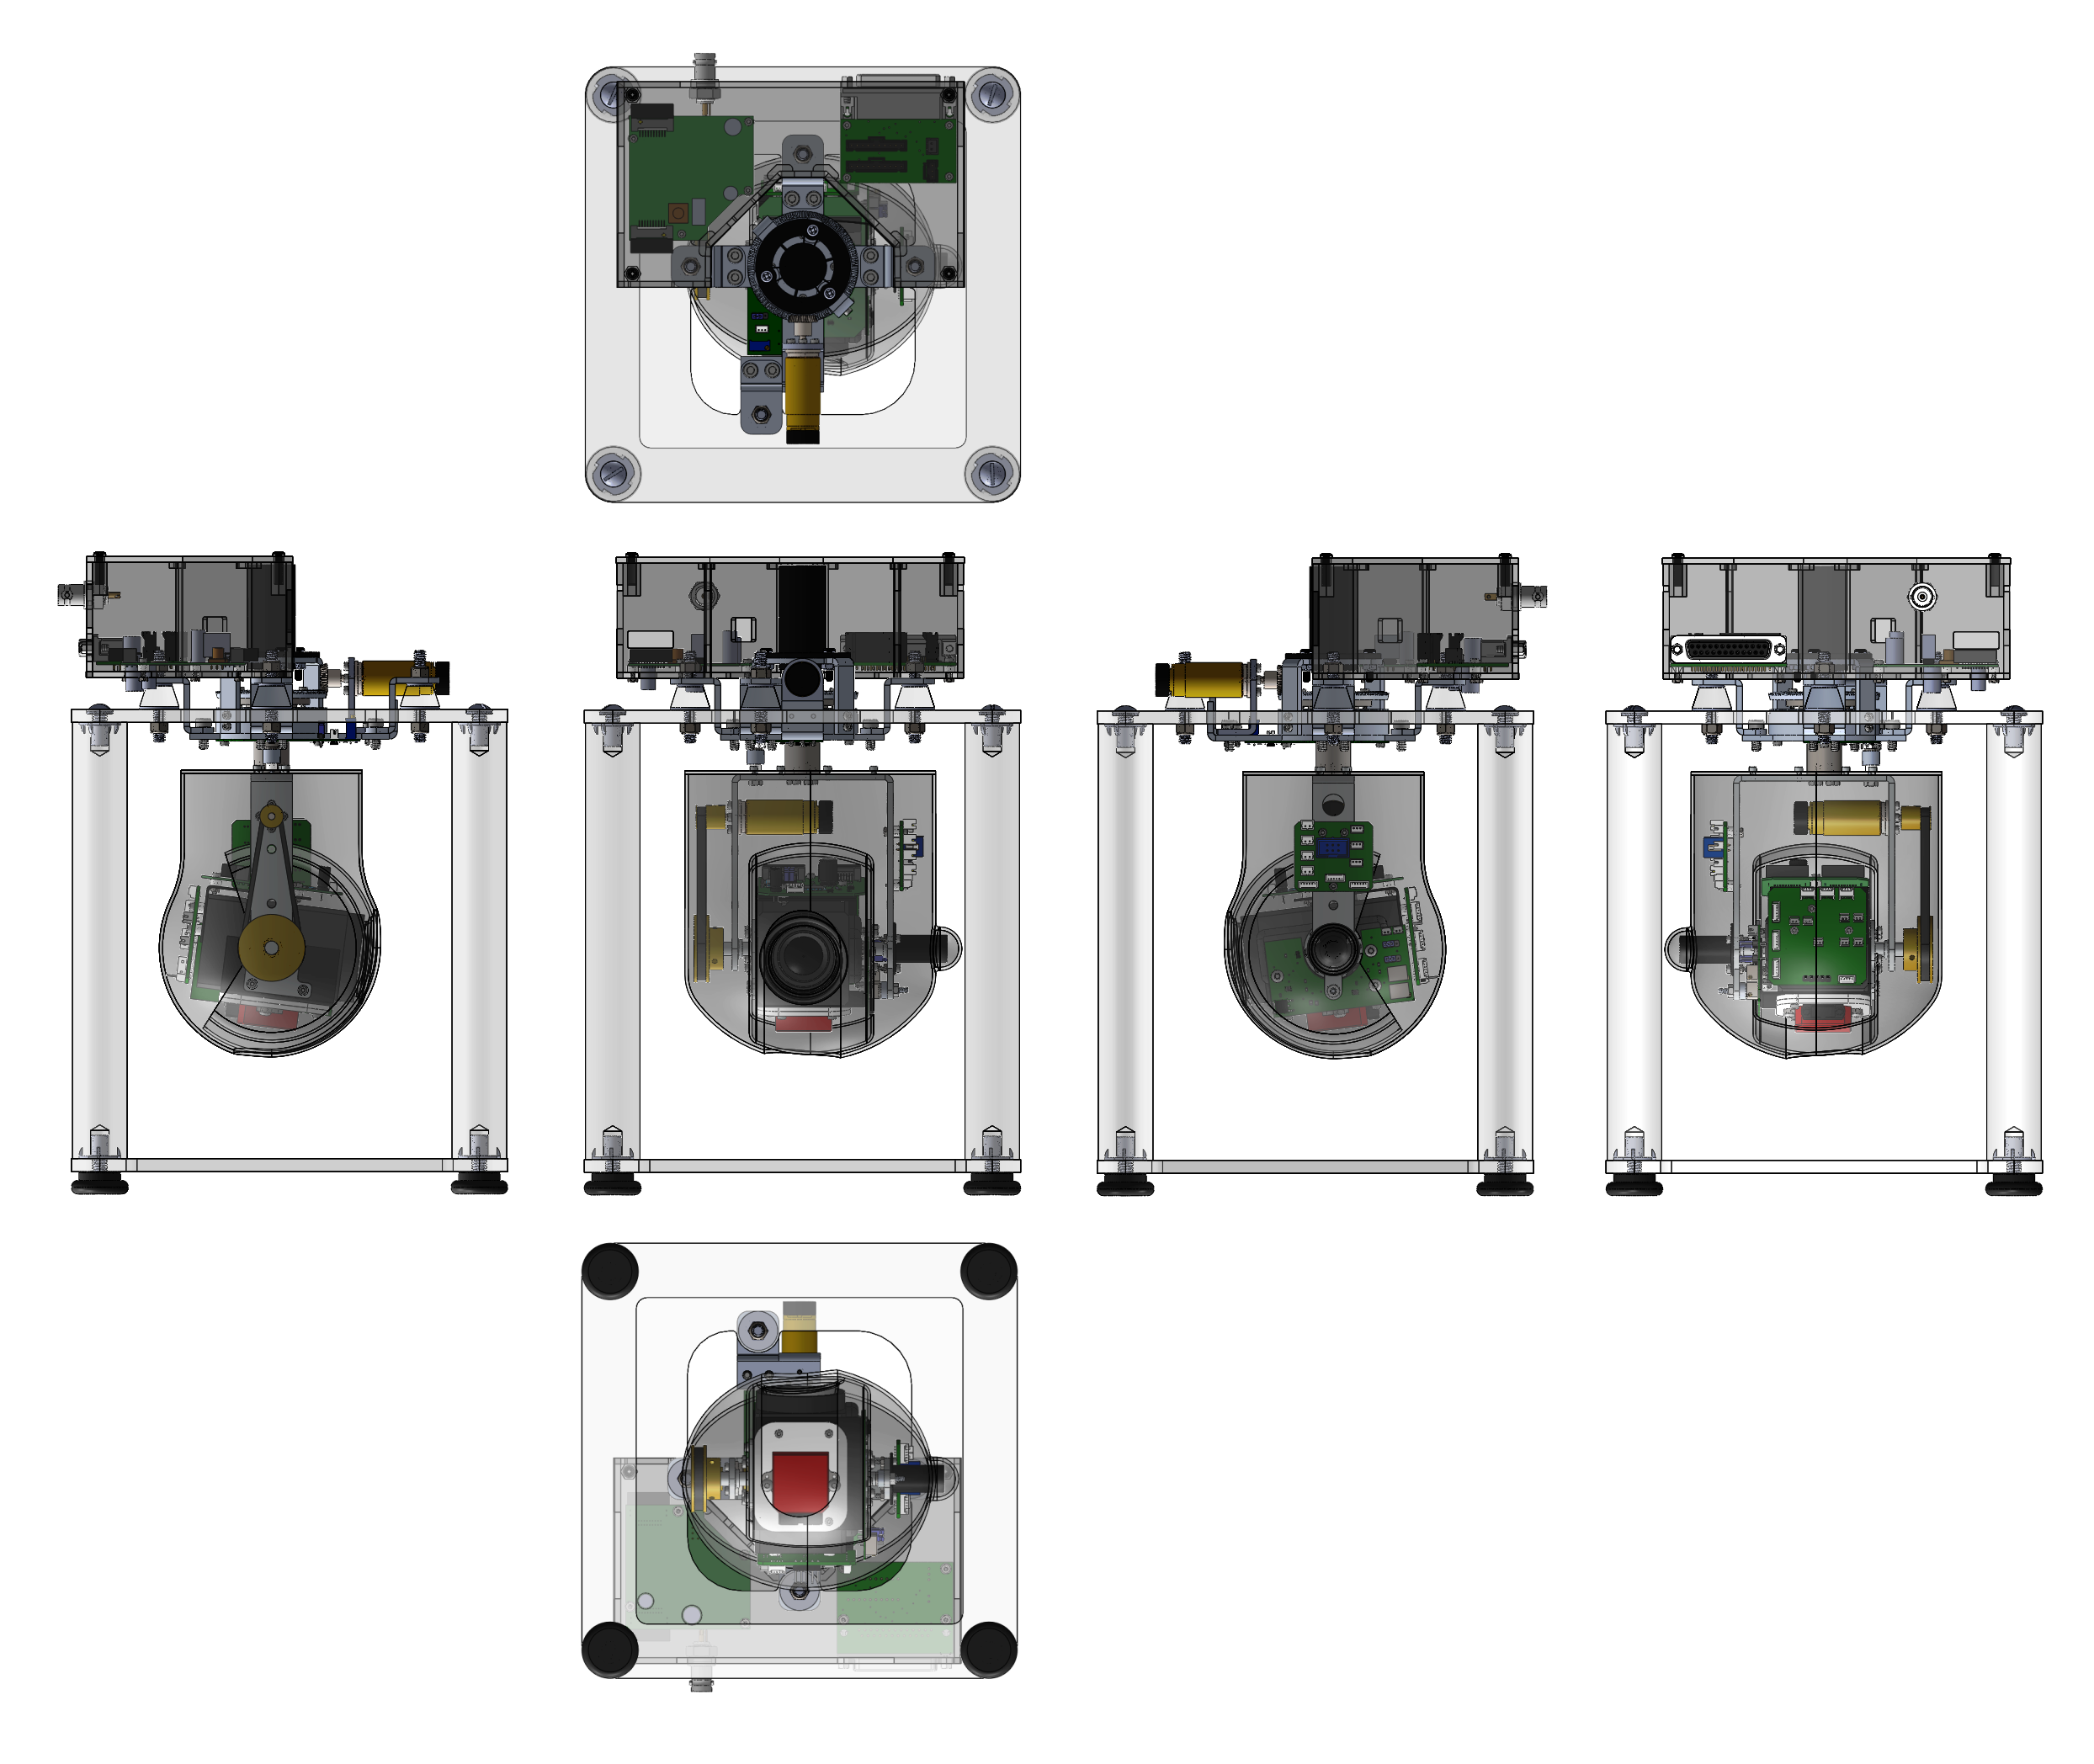
\includegraphics[scale=0.25]{img/GimbalViews.png}
%trim = izquierda abajo derecha arriba [scale=0.5,trim = 40mm 30mm 110mm 15mm, clip]
\caption{Vistas del Modelo 3D del Prototipo de C\'{a}mara Giroestablizada}%Esta es la l\'{i}nea para el pie de figura
\label{fig:GimbalViews}%esta es la etiqueta para referenciar en el texto la figura: ...como se aprecia de la Figura \ref{termopar}...
\end{figure}

Fueron necesarias modificaciones en el dise\~{n}o mec\'{a}nico original para mejorar las capacidades del sistema gimbal, una modificaci\'{o}n clave fue la instalaci\'{o}n de un slip ring\footnote{Un slip ring es un dispositivo electromec\'{a}nico que permite la transmici\'{o}n de energ\'{i}a o se\~{n}ales el\'{e}ctricas de una estructura estacionaria a una rotativa} en el eslab\'{o}n interno lo cual permite un giro de 360 grados y elimina las limitaciones causadas por los cables, derivada de esta modificaci\'{o}n tuvieron que dise\~{n}arse dos placas electr\'{o}nicas para la distribuci\'{o}n de se\~{n}ales entre la tarjeta de control en tilt y la tarjeta principal, ya que las conexiones disponibles en el slip ring eran menores de las necesarias. Finalmente para la f\'{a}cil manipulaci\'{o}n del sistema fue necesario dise\~{n}ar una base a la medida para el prototipo, la cual podemos ver en la figura ~\ref{fig:PrototipoTerminado}, La base est\'{a} fabricada en acr\'{i}lico de seis mil\'{i}metros cortado con l\'{a}ser y barra de una pulgada de di\'{a}metro, igualmente de acr\'{i}lico para los postes los cuales tienen injertos roscados de 1/4 de pulgada para poder ensamblarse, estos fueron insertados en la barra calentado los injertos de acero y posteriormente los postes fueron devastados en torno para que tuvieran una medida precisa. Esta base se dise\~{n}\'{o} y construy\'{o} con el fin de  manipular y almacenar del prototipo de forma segura.

\begin{figure}[H]
\centering 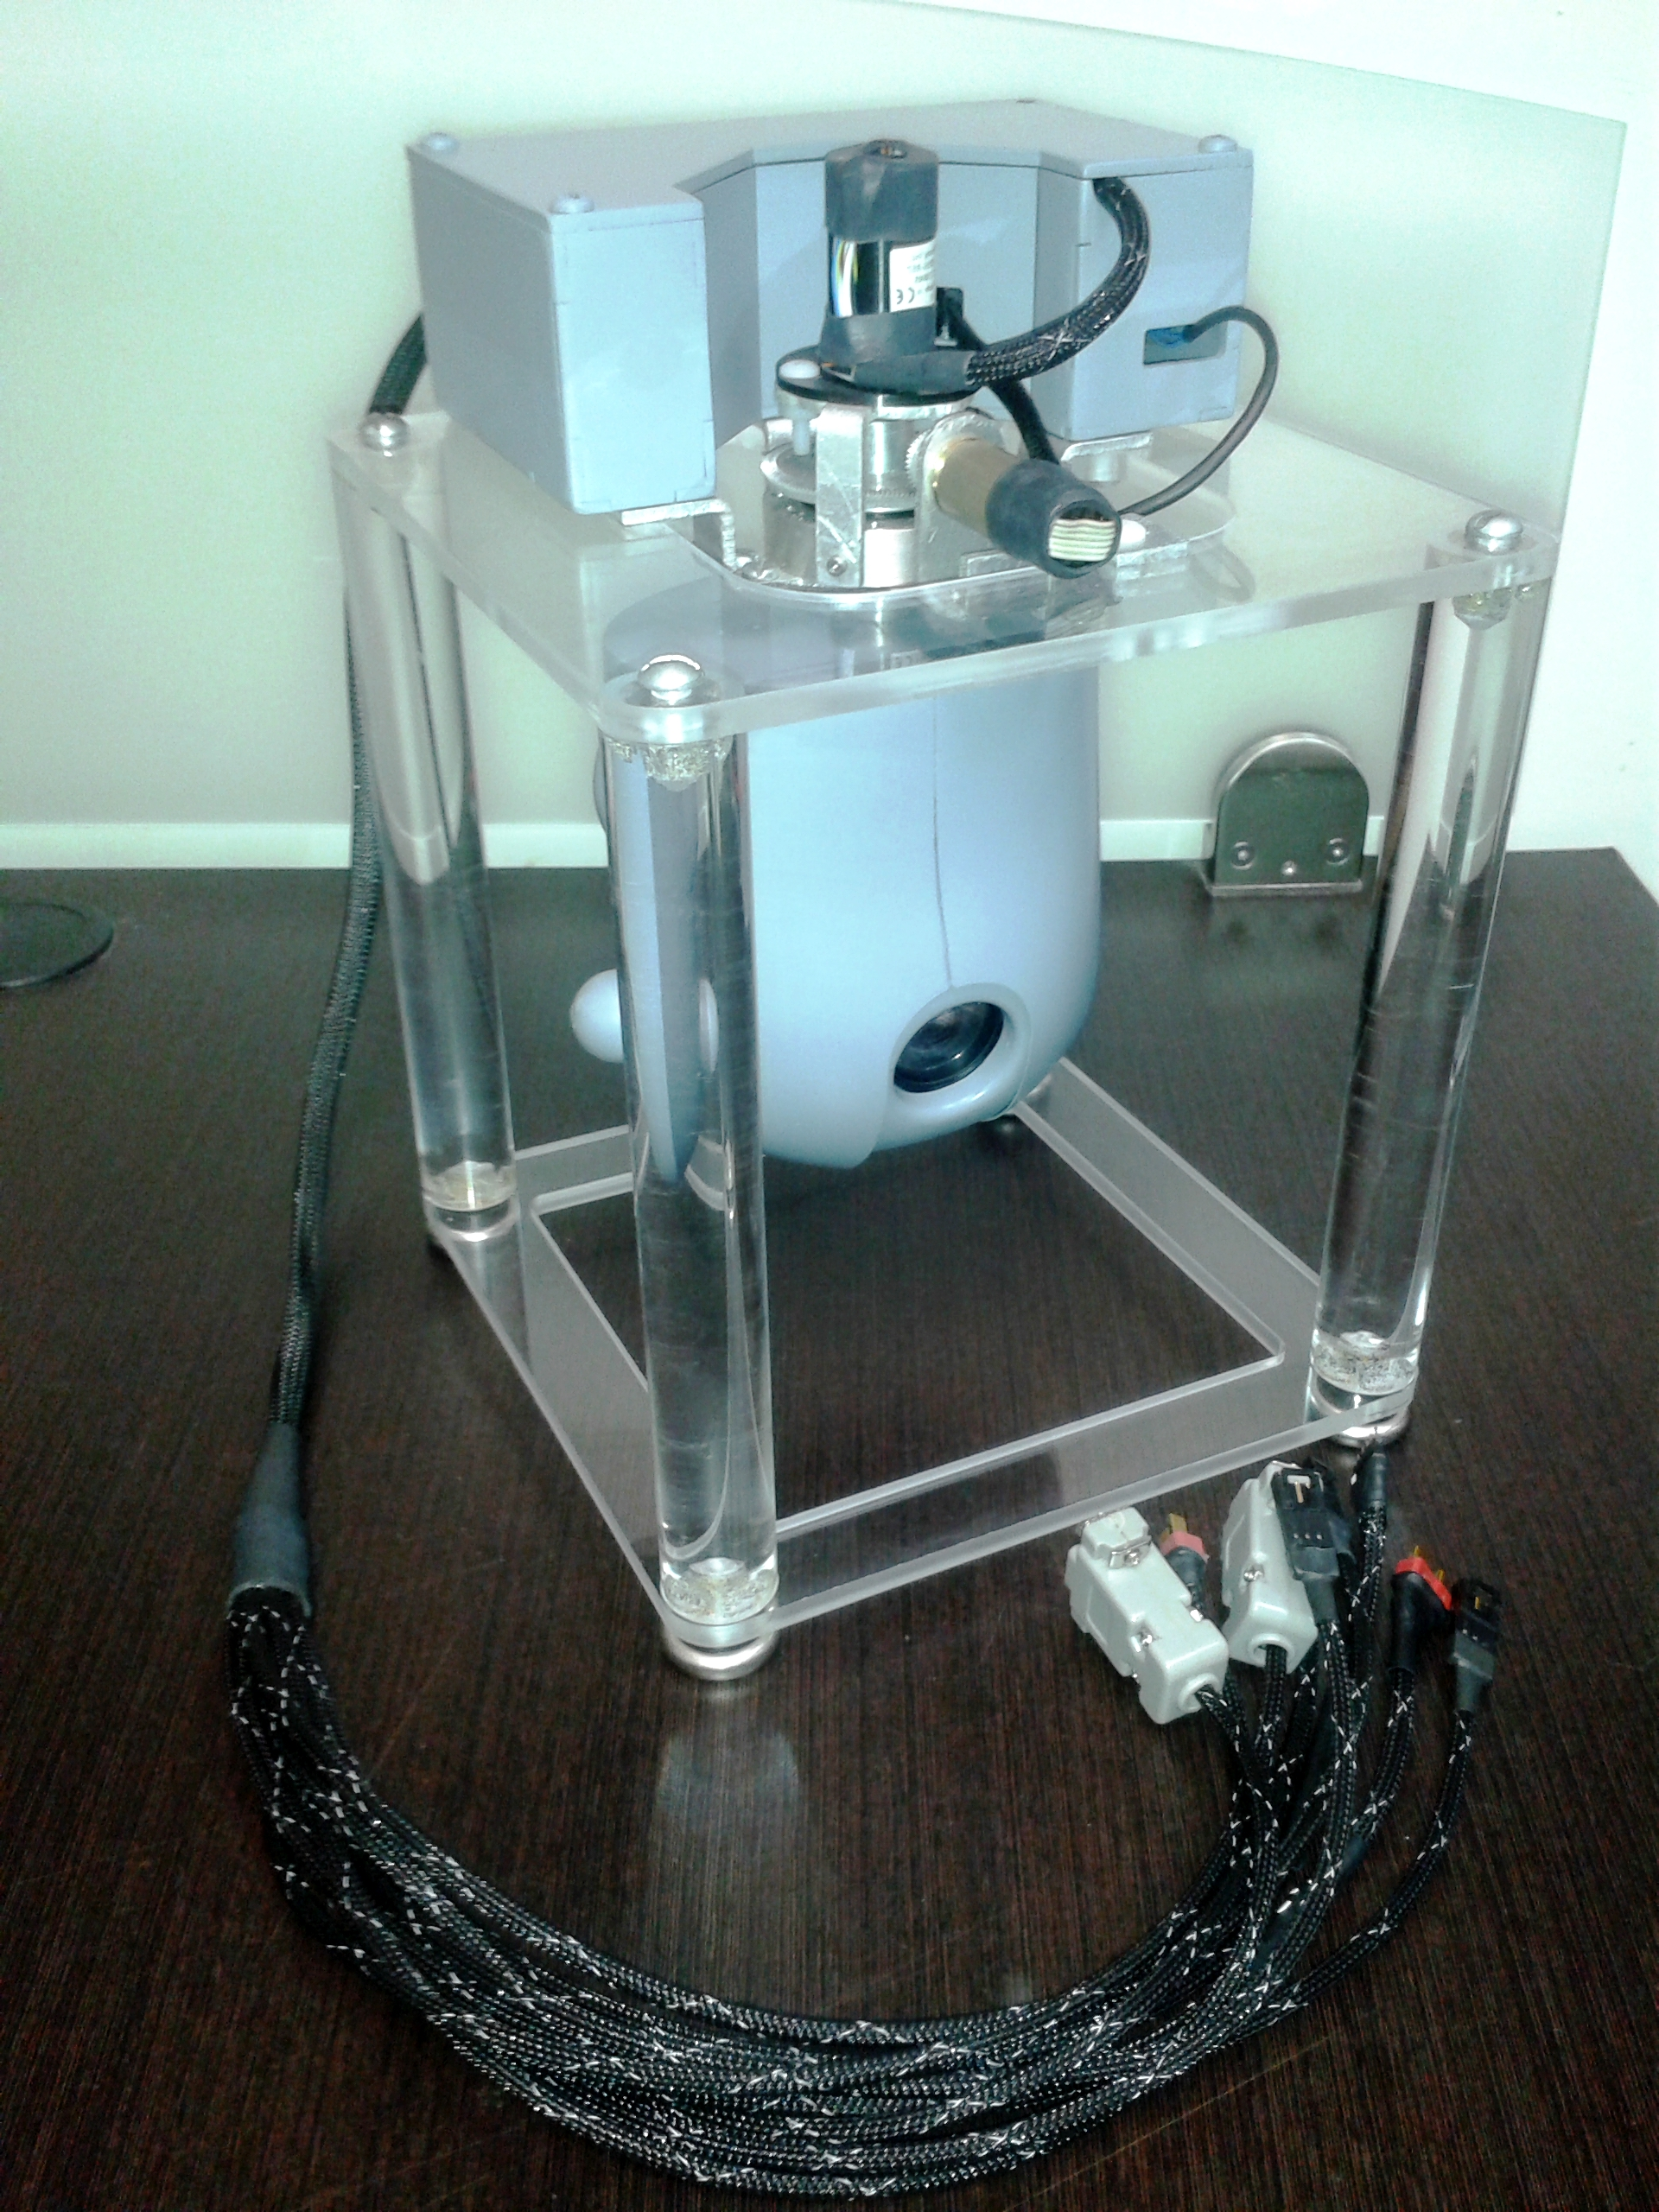
\includegraphics[scale=0.11]{img/PrototipoTerminado.jpg}
%trim = izquierda abajo derecha arriba [scale=0.5,trim = 40mm 30mm 110mm 15mm, clip]
\caption{Prototipo Terminado}
\label{fig:PrototipoTerminado}
\end{figure} 

\section{Electr\'onica}

\subsection{Tarjetas de Control}

Las tarjetas principales de control para el sistema fueron desarrolladas por el Dr. Mariano Lizarraga en el laboratorio de veh\'{i}culos aut\'{o}nomos del INIDETAM previo al inicio de esta tesis, podemos apreciar estas tarjetas en la figura ~\ref{fig:MainBoards}, la tarjeta del lado izquierdo es la \textit{"Main Board"} o tarjeta principal de control, la tarjeta de la derecha es la \textit{"Tilt Board"} o tarjeta de control de tilt. Sin embargo no se desarroll\'{o} el firmware\footnote{El firmware es un bloque de instrucciones de m\'{a}quina para prop\'{o}sitos espec\'{i}ficos, grabado en un chip, que establece la l\'{o}gica de m\'{a}s bajo nivel que controla los circuitos electr\'{o}nicos de un dispositivo y es el encargado de controlarlo para ejecutar correctamente las instrucciones externas} necesario para su funcionamiento, \'{u}nicamente se realiz\'{o} la programaci\'{o}n de controladores simples para algunos de sus perif\'{e}ricos. Por lo que esa tarea tuvo que llevarse a cabo como parte de esta tesis, este desarrollo se trata a detalle en la secci\'{o}n ~\ref{sec:Programacion}, en donde se describe el procedimiento y m\'{e}todo de programaci\'{o}n. 

\begin{figure}[H]
\centering
      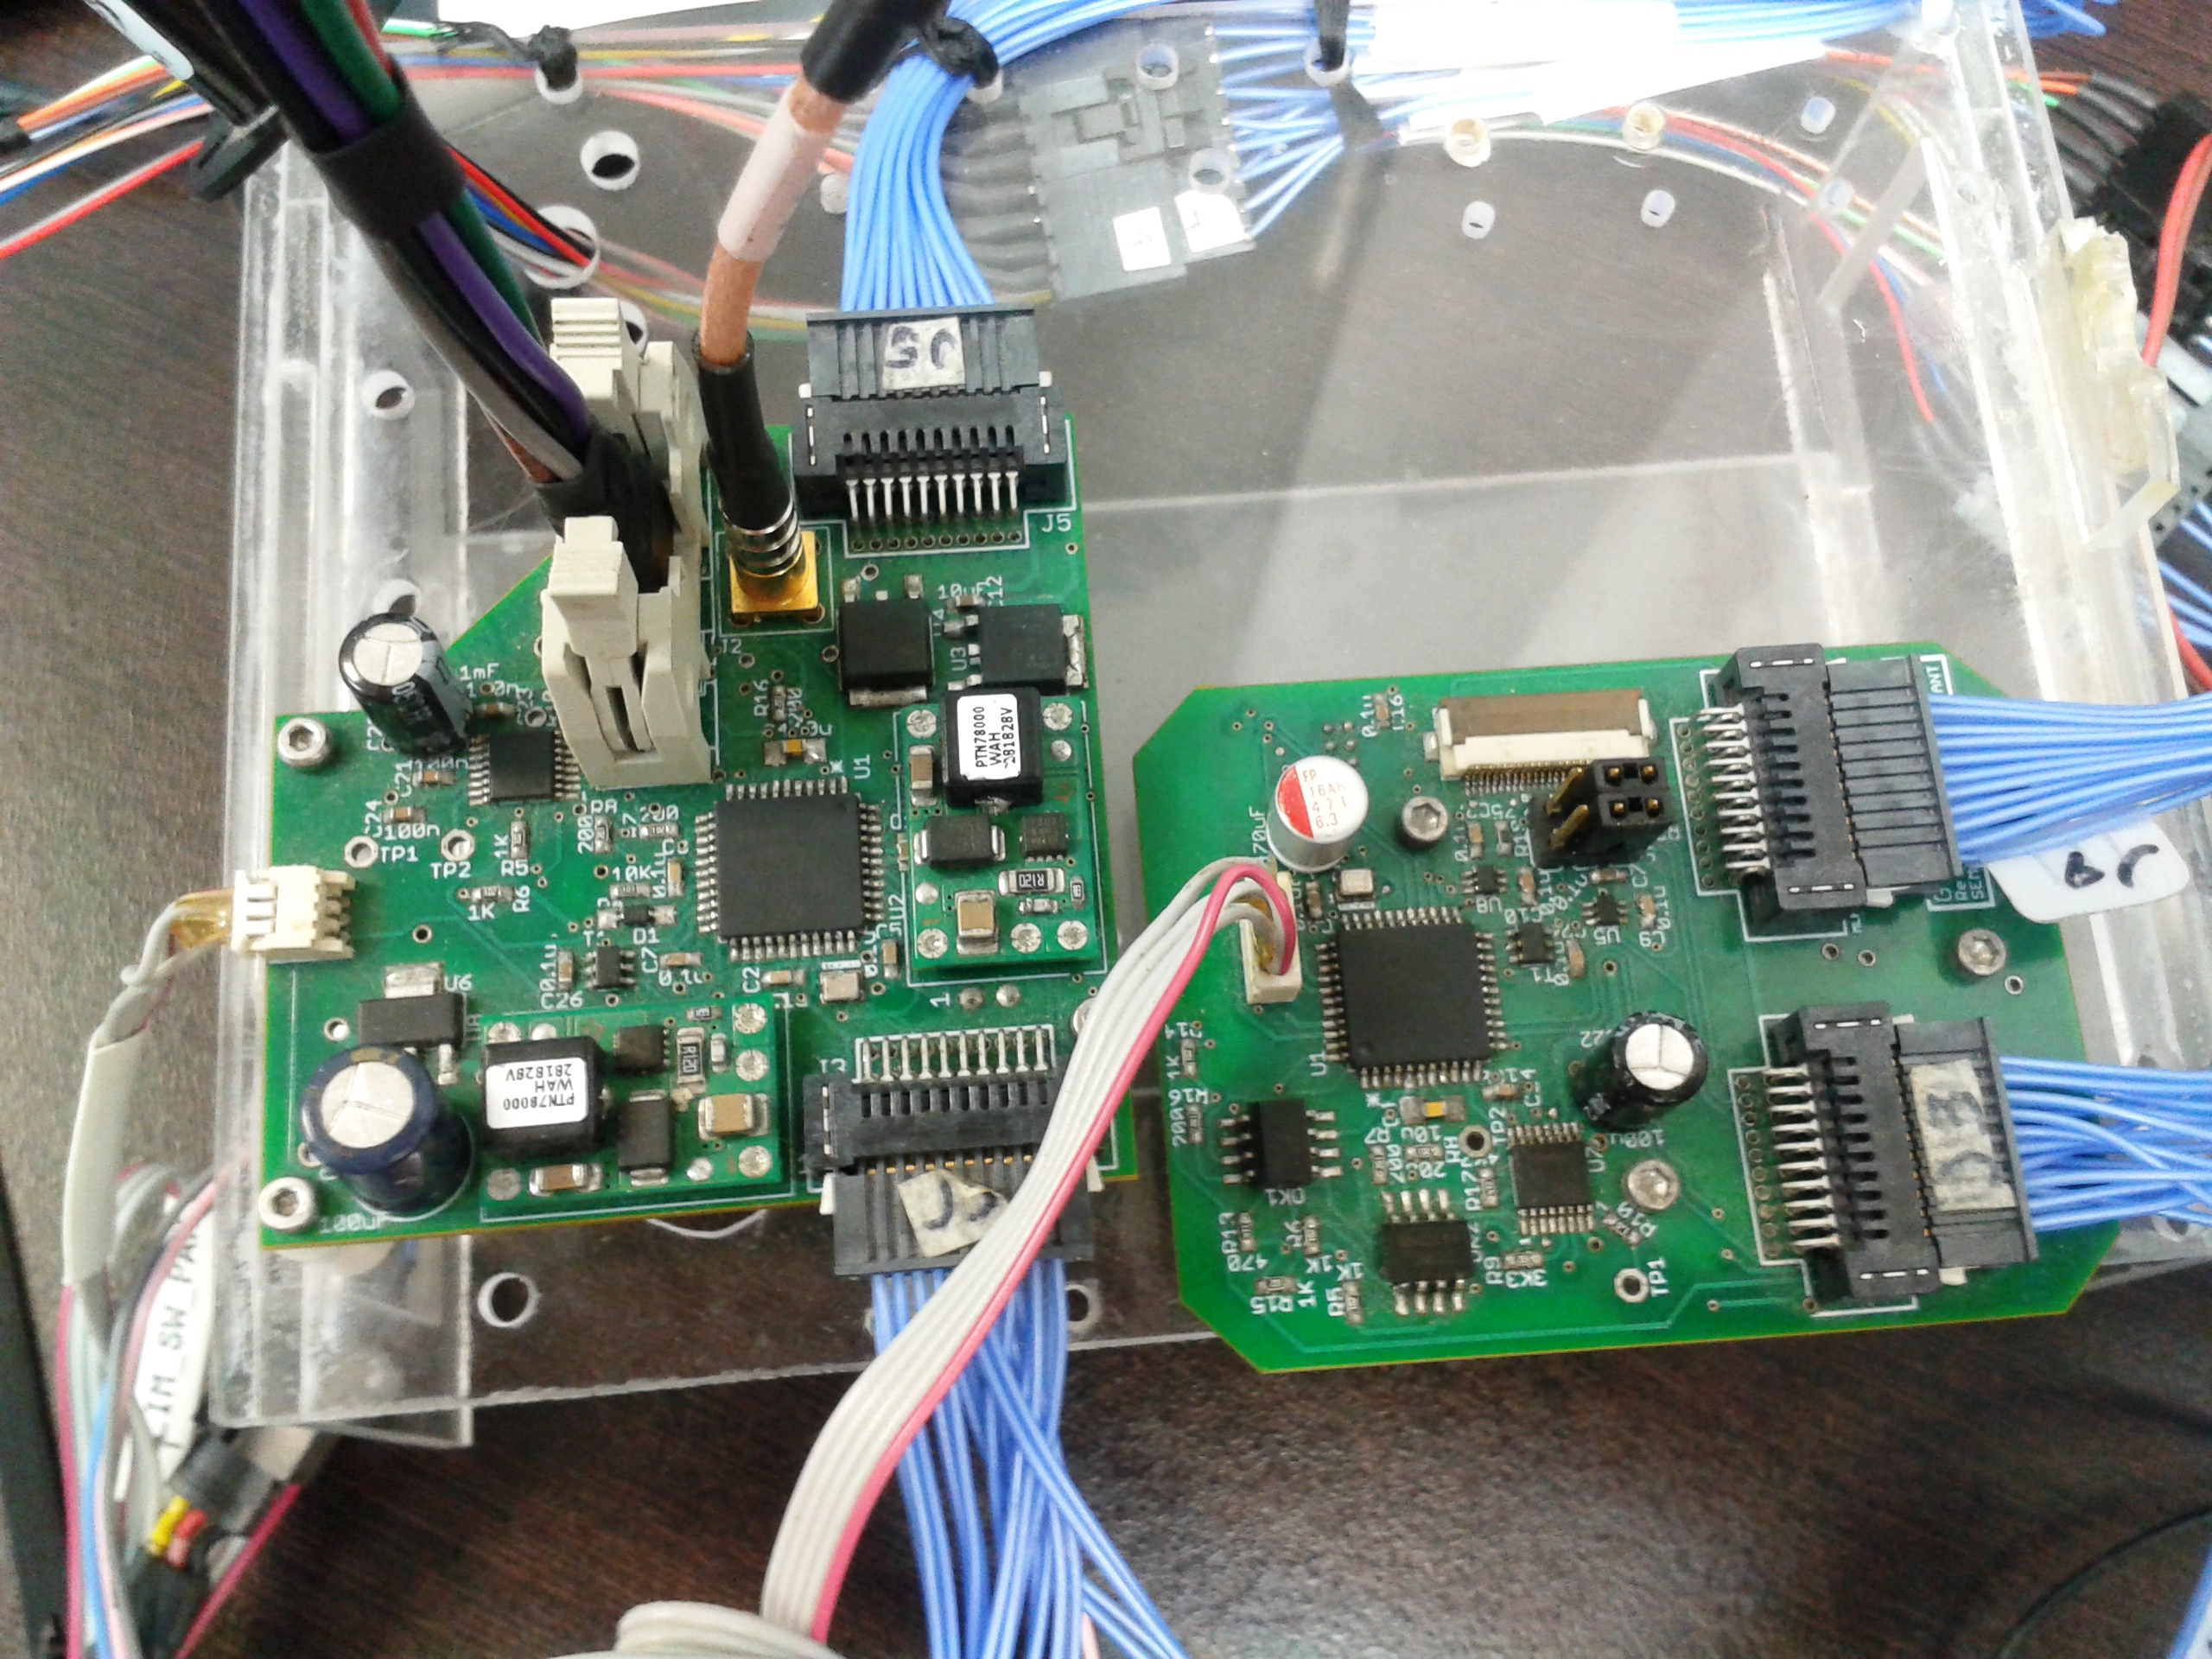
\includegraphics[scale=0.1]{img/Mainboards.jpg}
      \caption{Tarjetas Principales de Control del Sistema Montadas en el Banco de Pruebas}
      \label{fig:MainBoards}
\end{figure} 

La unidad de procesamiento central con el que cuentan estas tarjetas es un dsPIC33 de 16 bits. Estas tarjetas cuentan con todos los dispositivos electr\'{o}nicos necesarios para el control del sistema y a continuaci\'{o}n se describen sus caracter\'{i}sticas:\newline
\begin{large}
\textbf{Main Board} 
\end{large}

\begin{itemize}
    \item Procesador dsPIC33FJ128MC804 de 16 bits.
    \item Oscilador externo de 20 MHz.
    \item Transceptor de Bus CAN.
    \item Transceptor Serial RS232.
    \item Modulo de control para un encoder de cuadratura.
    \item Regulador interno de 24 v a 12 v para alimentaci\'{o}n de elementos de potencia.
    \item Reguladores internos de 12 v a 7 v, 5 v y 3.3 v para alimentaci\'{o}n de control.
    \item Salida regulada a 12 v y 7v.
    \item Driver para motor DC Texas Instruments\textsuperscript{\textregistered} DRV8801.
    \item Optoacoplamiento para aislamiento de la potencia de la l\'{o}gica de control.
    \item Sensor de Temperatura digital de 12 bits SPI.
    \item Conectores Samtec\textsuperscript{\textregistered} TFM-110-01-L-D para perif\'{e}ricos.
    \item Conector de v\'{i}deo Farnell\textsuperscript{\textregistered} MCX7-JPH-ST-TH1.
    \item Conexi\'{o}n a entrada digital para sensor de l\'{i}mite. 
    \item Programaci\'{o}n ICSP\footnote{Siglas para \textit{In-Circuit Serial Programming}, es la capacidad de algunos dispositivos l\'{o}gicos programables, microcontroladores y otros circuitos electr\'{o}nicos, de ser programados mientras est\'{a}n instalados en un sistema completo.}. 
\end{itemize}

\begin{large}
\textbf{Tilt Board} 
\end{large}

\begin{itemize}
    \item Procesador dsPIC33FJ128MC804 de 16 bits.
    \item Oscilador externo de 20 MHz.
    \item Dos m\'{o}dulos de comunicaci\'{o}n serial a 3.3 v.
    \item Modulo de control para un encoder de cuadratura.
    \item Dos conexi\'{o}n a entradas digitals para sensores de l\'{i}mite. 
    \item Reguladores internos de 7 v a 5v y 3.3v para alimentaci\'{o}n de control.
    \item Supresor de voltajes transitorios.
    \item Driver para motor DC Texas Instruments\textsuperscript{\textregistered} DRV8801.
    \item Optoacoplamiento para aislamiento de la potencia de la l\'{o}gica de control.
    \item Sensor de Temperatura digital de 12 bits SPI.
    \item Conectores Samtec\textsuperscript{\textregistered} TFM-110-01-L-D para perif\'{e}ricos.
    \item Conector tipo FFC de 0.5mm y 24 posiciones para interfaz con la c\'{a}mara SONY\textsuperscript{\textregistered} FCB-H11. 
    \item On-Screen Display\footnote{Es una imagen superpuesta sobre la pantalla de v\'{i}deo para mostrar informaci\'{o}n adicional.}.
    \item Programaci\'{o}n ICSP  
    \item Selector de l\'{i}nea para depuraci\'{o}n. 
    \item Capacidad para recepci\'{o}n de dos canales de v\'{i}deo con selector digital.
\end{itemize}


\subsection{C\'{a}mara}

La c\'{a}mara utilizada es la FCB-H11 de SONY\textsuperscript{\textregistered}, figura ~\ref{fig:Camara}, la cual es una c\'{a}mara de bloque de alta definici\'{o}n compatible con ocho formatos diferentes de v\'{i}deo que se muestran en la tabla ~\ref{Table:VideoFormat}, incluyendo el formato Full HD (1080i), que es equivalente a una se\~{n}al est\'{a}ndar de HD-TV. Las salidas de v\'{i}deo que maneja la c\'{a}mara son VBS\footnote{El v\'{i}deo compuesto es una se\~{n}al anal\'{o}gica de transmisi\'{o}n de v\'{i}deo en la que se codifica la imagen en sus diferentes componentes de luz y color a\~{n}adiendo los sincronismos necesarios para su posterior reconstrucci\'{o}n.} y Y/C\footnote{V\'{i}deo separado o s-video, es un tipo de se\~{n}al anal\'{o}gica de v\'{i}deo, tiene m\'{a}s calidad que el v\'{i}deo compuesto puesto que se separa la informaci\'{o}n del brillo y del color, mientras que en el v\'{i}deo compuesto se encuentran juntas.} para SD\footnote{Definici\'{o}n est\'{a}ndar, es la resoluci\'{o}n de v\'{i}deo dominante desde el origen de la TV hasta la aparici\'{o}n de la alta definici\'{o}n. El sistema est\'{a} alrededor de una resoluci\'{o}n de 500 l\'{i}neas horizontales.}  y componente anal\'{o}gico\footnote{V\'{i}deo por componentes es un t\'{e}rmino referido a la divisi\'{o}n de una se\~{n}al de v\'{i}deo en dos o m\'{a}s canales de componentes.} para HD\footnote{Alta definici\'{o}n, es un sistema de imagen, v\'{i}deo y/o sonido con mayor resoluci\'{o}n que la definici\'{o}n est\'{a}ndar, alcanzando resoluciones de 1280x720 p\'{i}xeles y 1920x1080 p\'{i}xeles.}. La c\'{a}mara est\'{a} equipada con un lente de zoom \'{o}ptico de enfoque autom\'{a}tico 10x y el zoom digital de 12x permite un zoom de hasta 120x, combinado con el zoom \'{o}ptico. 

\begin{figure}[H]
\centering 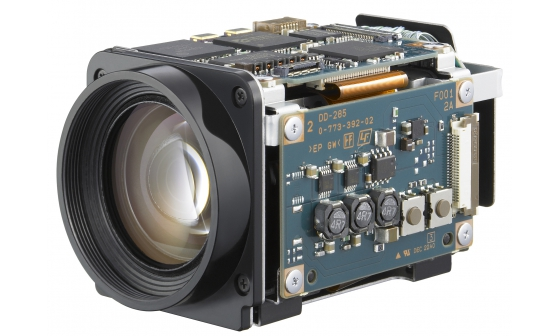
\includegraphics[scale=0.5]{img/Camara.jpeg}
\caption{SONY\textsuperscript{\textregistered} FCB-H11}
\label{fig:Camara}
\end{figure} 

La c\'{a}mara esta equipada con un filtro de infrarrojos dise\~{n}ado para reflejar o bloquear las longitudes de onda infrarroja dejando pasar \'{u}nicamente la luz del espectro visible. Este filtro puede ser desacoplado para incrementar la sensibilidad en ambientes de poca luz, a esta funci\'{o}n se le denomina Infrared Cutfilter Removal (ICR), El ICR se acoplar\'{a} autom\'{a}ticamente dependiendo de la luz ambiental, permitiendo a la c\'{a}mara ser efectiva en ambientes diurnos y nocturnos.

\begin{table}[h]
\caption{Formatos de V\'{i}deo de la C\'{a}mara FCB-H11}
\label{Table:VideoFormat}
\begin{center}
\begin{tabular}{ |l|l|l| }
\hline
\multicolumn{2}{ |c| }{Formatos de V\'{i}deo Soportados} \\
\hline
Tipo & Formato\\ \hline
\multirow{4}{*}{HD} 
 & 1080i/59.94\\
 & 1080i/50\\
 & 720p/59.94\\
 & 720p/50\\ 
 \hline
\multirow{4}{*}{SD} 
 & NTSC\footnotemark{}(Crop)\\
 & NTSC(squeeze)\\
 & PAL\footnotemark{}(Crop)\\ 
 & PAL(Squeeze)\\ 
\hline
\end{tabular}
\end{center}
\end{table}

\addtocounter{footnote}{-2}
\stepcounter{footnote}\footnotetext{Llamado as\'{i} por las siglas de \textit{National Television System Committee}. Es un sistema de codificaci\'{o}n utilizado para la transmisi\'{o}n de sistemas de televisi\'{o}n anal\'{o}gica, que consiste en 29.97 cuadros de v\'{i}deo por segundo con exploraci\'{o}n entrelazada.}
\stepcounter{footnote}\footnotetext{Sigla de \textit{Phase Alternating Line}. Es un sistema de codificaci\'{o}n utilizado para la transmisi\'{o}n de sistemas de televisi\'{o}n anal\'{o}gica en la que primero se exploran las l\'{i}neas impares y luego las pares.}

La c\'{a}mara utiliza el protocolo de comunicaciones VISCA, de sus siglas en ingl\'{e}s \textit{Video System Control Architecture}, el cual es un protocolo profesional para c\'{a}maras de vigilancia basado en RS232 con paquetes de los 3 a los 16 bytes desarrollado por SONY\textsuperscript{\textregistered}, el cual permite controlar la c\'{a}mara desde una computadora. Es posible seleccionar un amplio rango de velocidades de comunicaci\'{o}n de entre los 9600 bps, 19200 bps, o 38400 bps. Esto permite controlar la c\'{a}mara remotamente a una alta velocidad de comunicaci\'{o}n. La c\'{a}mara incluye la funci\'{o}n de posici\'{o}n de preajuste, lo que le permite guardar hasta seis diferentes configuraciones de las condiciones de captura de la c\'{a}mara, para poder elegir el comportamiento de la c\'{a}mara al encenderse. 

\subsection{Unidad de Medici\'{o}n Inercial}

La unidad de medici\'{o}n inercial (IMU) por sus siglas en ingl\'{e}s utilizada es la \textit{VN-100 Rugged} de VectorNav\textsuperscript{\textregistered}, figura ~\ref{fig:IMU}, que consiste en sensor VN-100 el cual tiene un CPU de 32 bits y varios sensores de estado s\'{o}lido integrados; un aceler\'{o}metro de tres ejes, un giroscopio de tres ejes, un magnet\'{o}metro de tres ejes y un sensor barom\'{e}trico de presi\'{o}n. Tiene una carcasa robusta de aluminio de alta precision de 36 x 33 x 9 mm con un conector de 10 pines y dos interfaces de comunicaci\'{o}n serial f\'{i}sicamente separadas RS232. 

\begin{figure}[H]
\centering 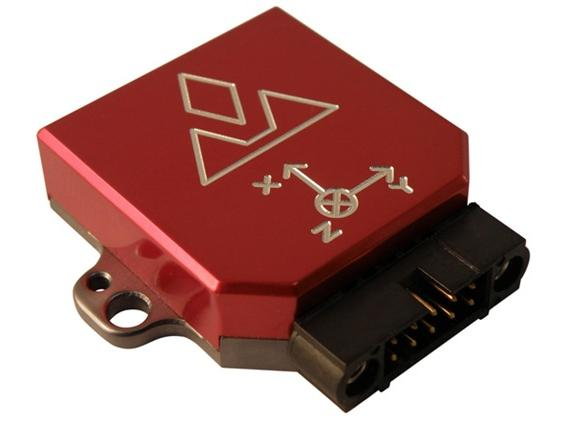
\includegraphics[scale=0.4]{img/VN100.jpg}
\caption{Central Inercial VectorNav\textsuperscript{\textregistered}}
\label{fig:IMU}
\end{figure} 

La arquitectura de software interna del VN-100 consiste en cuatro subsistemas separados. Estos subsistemas son la IMU, el NavState, el NavFilter y la interfase de comunicaciones. El subsistema de la IMU se ejecuta a la velocidad m\'{a}s alta del sistema (800Hz), este es el subsistema responsable de recolectar las mediciones brutas, aplicar calibraciones a las mediciones, aplicar una rotaci\'{o}n al marco de referencia y opcionalmente filtrar la se\~{n}al individual de cada sensor. El subsistema NavState, genera un flujo de datos continuo producido por el algoritmo de estimaci\'{o}n de la orientaci\'{o}n el cual es un filtro de Kalman extendido basado en quaterniones que provee un rango de movimiento completo de 360 grados y puede configurarse a una velocidad m\'{a}xima de 400Hz. El subsistema NavFilter consiste en un VPE\footnote{Son las siglas de \textit{Vector Processing Engine}. Un procesador vectorial es un dise\~{n}o de CPU capaz de ejecutar operaciones matem\'{a}ticas sobre m\'{u}ltiples datos de forma simult\'{a}nea.} y una variedad de filtros Kalman que se ejecutan a una velocidad menor que el subsistema NavState (200Hz). La interfase de comunicaciones que provee el sensor VN-100 consiste en dos interfases seriales UART\footnote{Siglas en ingl\'{e}s para Transmisor-Receptor As\'{i}ncrono Universal, es el dispositivo que controla los puertos y dispositivos serie.} bidireccionales f\'{i}sicamente separadas y un bus SPI. Cada interfaz UART soporta velocidades desde los 9600 bps hasta un m\'{a}ximo de 921600 bps. Las interfaces UART trabajan a voltajes TTL\footnote{Siglas en ingl\'{e}s de l\'{o}gica transistor a transistor. Es una tecnolog\'{i}a de construcci\'{o}n de circuitos electr\'{o}nicos digitales en que  los elementos de entrada y salida del dispositivo son transistores bipolares.} de 3 v, sin embargo el VN-100 Rugged tiene un tranceptor que permite usar una interfaz serial a voltajes serial RS232 est\'{a}ndar. El protocolo de comunicaci\'{o}n usado por el VN-100 puede configurarse para ser un protocolo binario o ASCII\footnote{Acr\'{o}nimo del ingl\'{e}s para C\'{o}digo Est\'{a}ndar Estadounidense para el Intercambio de Informaci\'{o}n, es un c\'{o}digo de caracteres basado en el alfabeto latino, tal como se usa en ingl\'{e}s moderno.} basado en comandos y polling\footnote{Es la operaci\'{o}n de consulta constante, generalmente hacia un dispositivo de hardware, para crear una actividad sincr\'{o}nica sin el uso de interrupciones.} de registros. El protocolo ASCII es muy similar al protocolo NMEA 0183 ampliamente utilizado por la mayor\'{i}a de los receptores GPS y consiste par\'{a}metros separados por una coma impresos en texto legible por un humano. En la figura ~\ref{fig:VN100Responce} se muestra un ejemplo del comando de solicitud y respuesta del VN-100 en protocolo ASCII.

\begin{figure}[H]
\centering 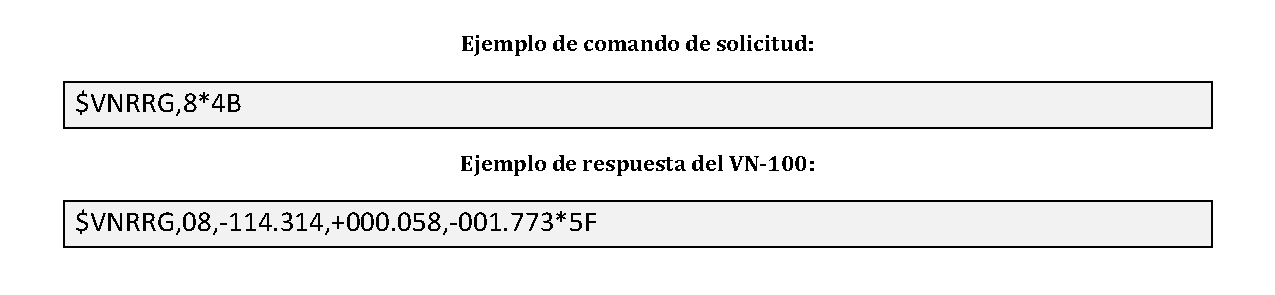
\includegraphics[scale=0.8]{img/VN100Responce.pdf}
\caption{Ejemplo del Protocolo de Comunicaci\'{o}n del VN-100}
\label{fig:VN100Responce}
\end{figure} 

\subsection{Motor}

El motor utilizado para el control de ambos eslabones es el 1524T012SR de la empresa alemana FAULHABER \textsuperscript{\textregistered}, figura ~\ref{fig:motor}, Estos motores utilizan un sistema patentado de bobinado sin n\'{u}cleo que ofrece una mayor potencia y mejor desempe\~{n}o din\'{a}mico al menor peso y tama\~{n}o posible. Entre los beneficios de ofrece \'{e}sta tecnolog\'{i}a est\'{a}n:

\begin{itemize}
    \item Eliminaci\'{o}n del par de reluctancia lo que resulta en un posicionamiento m\'{a}s suave y control de velocidad con una eficiencia m\'{a}s alta que otro tipo de motores.
    \item Par y potencia muy alto en relaci\'{o}n con su peso y tama\~{n}o.
    \item Relaci\'{o}n linear entre carga y velocidad, corriente y par, y voltaje y velocidad.
    \item Muy baja inercia del rotor lo que resulta en una din\'{a}mica superior en el arranque y paro del motor.
\end{itemize}

\begin{figure}[H]
\centering 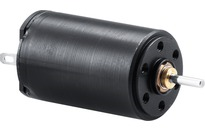
\includegraphics[scale=0.01]{img/motor.png}
\caption{FAULHABER\textsuperscript{\textregistered} 1524T012SR}
\label{fig:motor}
\end{figure} 

Este motor tiene una conmutaci\'{o}n de metales preciosos, esto se refiere a los materiales usados en las escobillas y el conmutador consisten en aleaciones de metales preciosos de alto desempe\~{n}o. Este tipo de sistema de conmutaci\'{o}n es usado principalmente debido a su peque\~{n}o tama\~{n}o, muy baja fricci\'{o}n y una se\~{n}al precisa de conmutaci\'{o}n. En general los motores con conmutaci\'{o}n de metales preciosos exhiben el mejor desempe\~{n}o. Los par\'{a}metros del motor se resumen en la tabla ~\ref{Table:MotorParameters}.

\begin{table}[H]
\caption{Par\'{a}metros del Motor}
\label{Table:MotorParameters}
\begin{center}
\begin{tabular}{ |l|c| }
\hline
 \multicolumn{2}{ |c| }{\textbf{Par\'{a}metros del Motor FAULHABER\textsuperscript{\textregistered} 1524T012SR}} \\
\hline
\textit{Par\'{a}metro} & \textit{Valor} \\
\hline
Voltaje Nominal & 12 v  \\
Resistencia T\'{e}rmica & 19.8 $\Omega$  \\
Potencia de Salida & 1.75 W  \\
Eficiencia M\'{a}xima & 76 \%  \\
Velocidad sin carga & 9900 rpm  \\
Corriente sin carga & 0.011 A  \\
Par de Fricci\'{o}n & 0.13 mNm  \\
Constante de Velocidad & 840 rpm/v \\
Constante de Par & 11.4 mNm/A \\
Constante de Corriente & 0.088 A/mNm \\
Inductancia del Rotor & 250 $\mu$H \\
Constante de Tiempo Mec\'{a}nica & 10 ms \\
Inercia del Rotor & 0.65 g cm\textsuperscript{2}\\
Aceleraci\'{o} Angular & 100x10\textsuperscript{3} rad/s\textsuperscript{2} \\
Peso & 21 g \\
Material Magnetico & NdFeB\\
\hline
\end{tabular}
\end{center}
\end{table}
 

Adicionalmente se ha equipado al motor con un moto-reductor FAULHABER\textsuperscript{\textregistered} serie 15/5 con una caja de engranes de tres etapas y una relaci\'{o}n 21:1 que le a\~{n}ade un par adicional al motor. Tambi\'{e}n tiene un encoder incremental de cuadratura FAULHABER\textsuperscript{\textregistered} IE2-512 acoplado a la flecha del motor, sus caracter\'{i}sticas se muestran en la tabla ~\ref{Table:EncParameters}. Finalmente el arreglo final usado se muestra en la figura ~\ref{fig:ArrMotor}.

\begin{table}[H]
\caption{Caracter\'{i}sticas del Encoder}
\label{Table:EncParameters}
\begin{center}
\begin{tabular}{ |l|c| }
\hline
 \multicolumn{2}{ |c| }{\textbf{Caracter\'{i}sticas del Encoder FAULHABER\textsuperscript{\textregistered} IE2-512}} \\
\hline
\textit{Par\'{a}metro} & \textit{Valor} \\
\hline
Resoluci\'{o}n & 512 PPR  \\
Frecuencia M\'{a}xima & 160 kHz  \\
Voltaje de Alimentaci\'{o}n & 4.5 - 5.5 v  \\
Corriente M\'{a}xima & 13 mA  \\
Desfase ente Canal A y B & 90$^\circ$  \\
Inercia del disco & 0.09 g cm\textsuperscript{2}  \\
\hline
\end{tabular}
\end{center}
\end{table}

\begin{figure}[H]
\centering 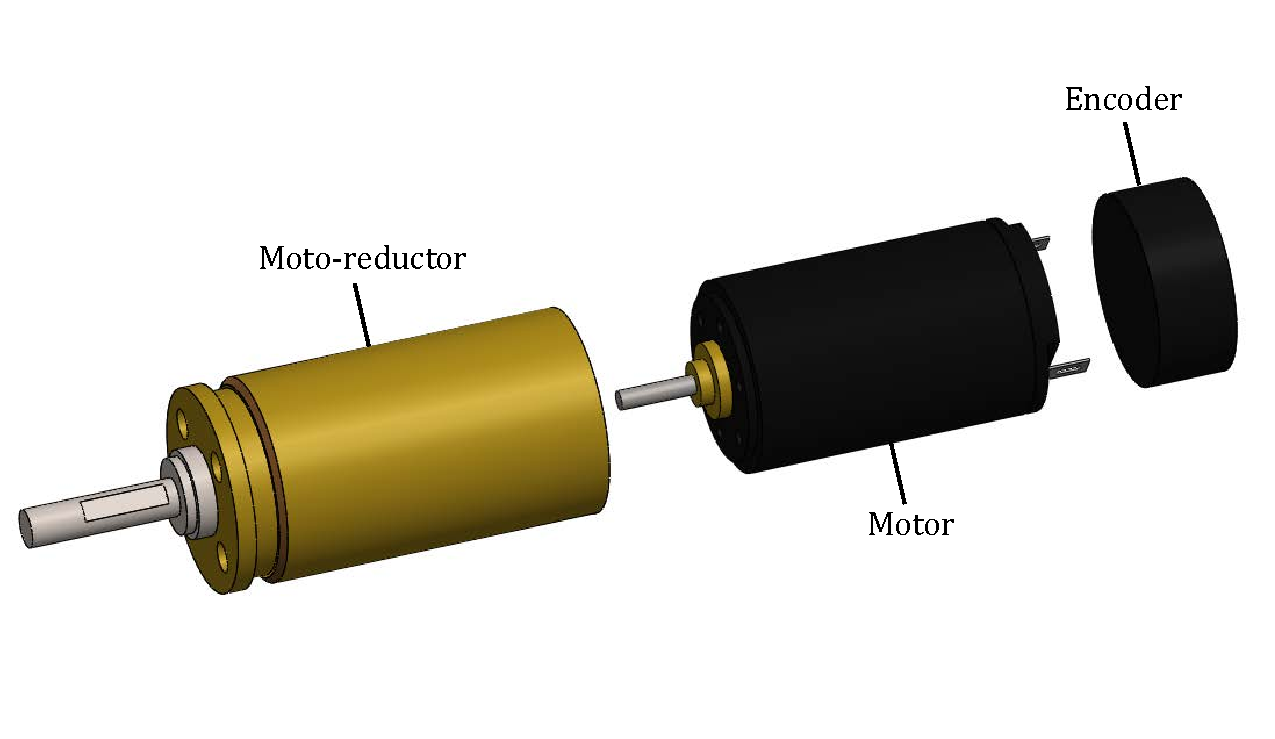
\includegraphics[scale=0.52]{img/ArrMotor.pdf}
\caption{Arreglo Moto-reductor - Motor - Encoder usado en el Sistema}
\label{fig:ArrMotor}
\end{figure}

\subsection{Sensores de l\'{i}mite}

El sistema esta l\'{i}mitado en su rango de movimiento en el eslab\'{o}n interno a 90$^\circ$ debido principalmente al dise\~{n}o de la carcasa, figura ~\ref{fig:LimTilt}. Para asegurar que el sistema \'{u}nicamente trabajar\'{a} en el rango establecido por las l\'{i}mitaciones mec\'{a}nicas se ha dise\~{n}ado un sensor que detecte cuando el \'{a}ngulo de elevaci\'{o}n ha llegado a su l\'{i}mite. Para no a\~{n}adir elementos mec\'{a}nicos extras se ha optado por usar un sensor magn\'{e}tico de efecto Hall para detectar la posici\'{o}n l\'{i}mite de la c\'{a}mara. 

\begin{figure}[H]
\centering 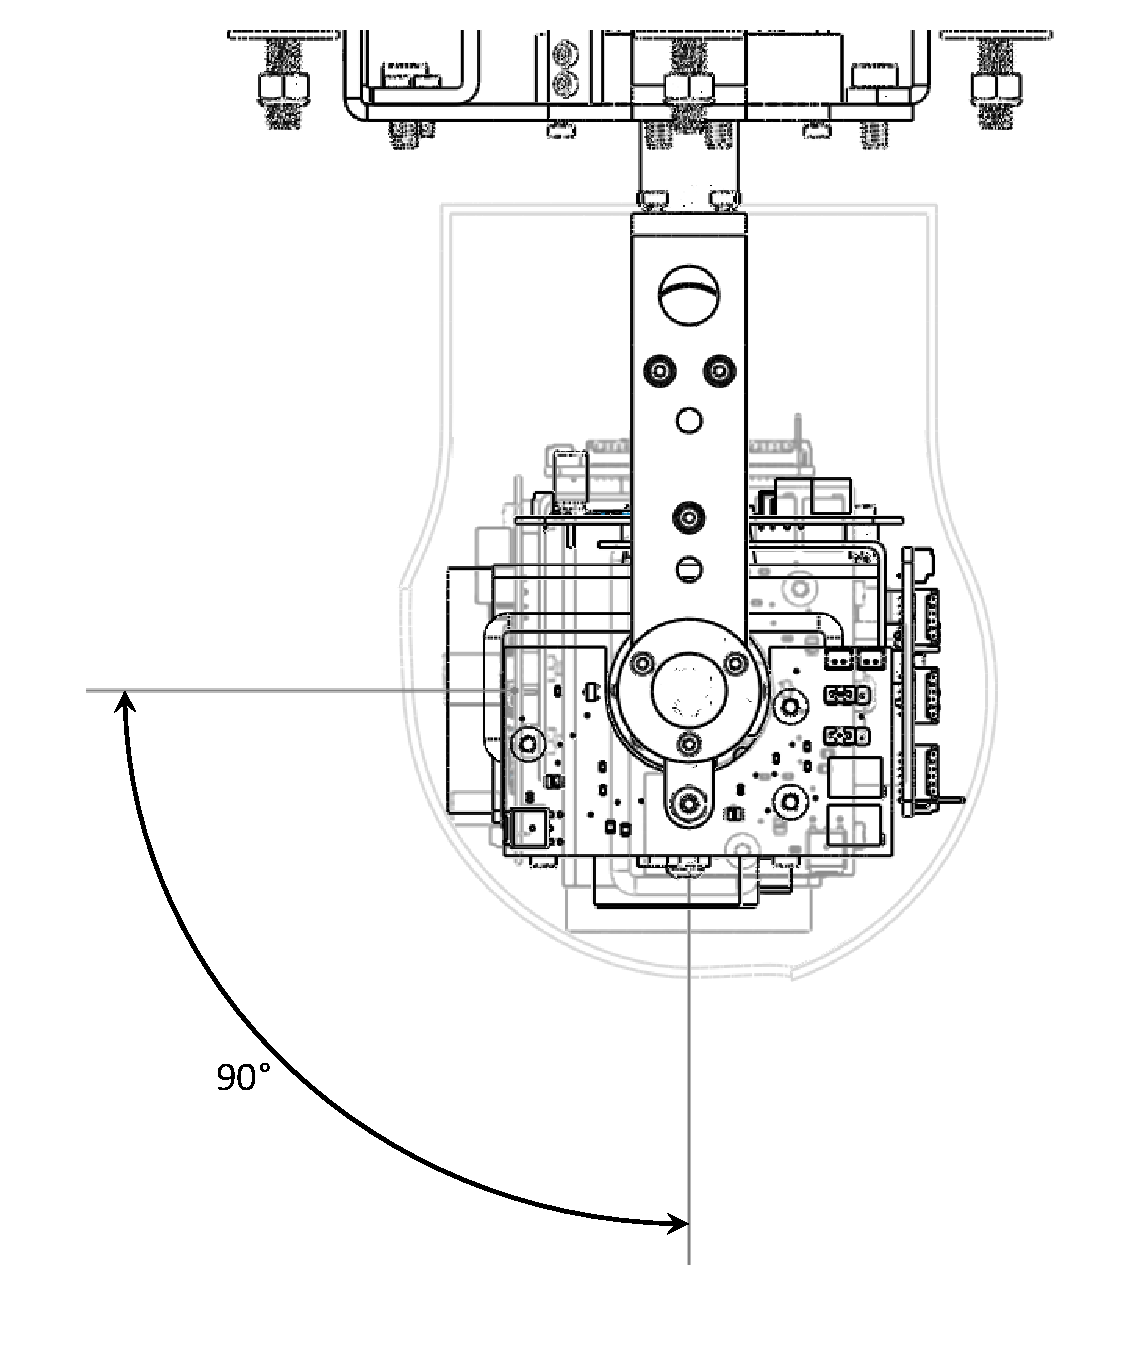
\includegraphics[scale=0.45,trim = 0mm 20mm 0mm 0mm]{img/Limit.pdf}
%trim = izquierda abajo derecha arriba [scale=0.5,trim = 40mm 30mm 110mm 15mm, clip]
\caption{L\'{i}mite Tilt}
\label{fig:LimTilt}
\end{figure} 

Estos sensores se basan en el descubrimiento realizado el Dr. Edwin Hall en 1879, el cual dice que \textit{"Cuando un conductor por que esta circulando una corriente, es expuesto a un campo magn\'{e}tico, se generar\'{a} un voltaje perpendicular a ambos, al flujo de corriente y al campo magn\'{e}tico"}, en su honor se nombro a este el "Efecto Hall", el efecto Hall puede aplicarse a muchos tipos de dispositivos sensores, mientras el par\'{a}metro a medir involucre o pueda involucrar un campo magn\'{e}tico. El voltaje generado por este efecto es muy peque\~{n}o, en el orden de los microvoltios por lo que se requiere de electr\'{o}nica adicional para alcanzar niveles de voltaje pr\'{a}cticos. En el mercado existen dos tipos de sensores efecto Hall: anal\'{o}gicos y digitales, los sensores anal\'{o}gicos proveen una salida anal\'{o}gica de voltaje que es proporcional a la intensidad del campo magn\'{e}tico. La salida de los sensores digitales es discreta, unicamente dos niveles, es decir 1 o 0, nunca en medio y no puede modificarse la magnitud del campo magn\'{e}tico que cambia su estado. Para poder ajustar la precision del sensor, se seleccion\'{o} un sensor de efecto Hall anal\'{o}gico radiom\'{e}trico que provee una salida estable y alta sensibilidad, adem\'{a}s de responder a campos magn\'{e}ticos positivos y negativos. Se dise\~{n}\'{o} la electr\'{o}nica necesaria para el tratamiento de la se\~{n}al, que consiste en un comparador de alta precisi\'{o}n con hist\'{e}resis\footnote{Tendencia de un material a conservar una de sus propiedades, en ausencia del est\'{i}mulo que la ha generado.} ajustable, figura ~\ref{fig:EsqTilt}, este circuito nos permite calibrar de forma precisa la sensibilidad del sensor y producir la se\~{n}al digital que necesita el control.  

\begin{figure}[H]
\centering 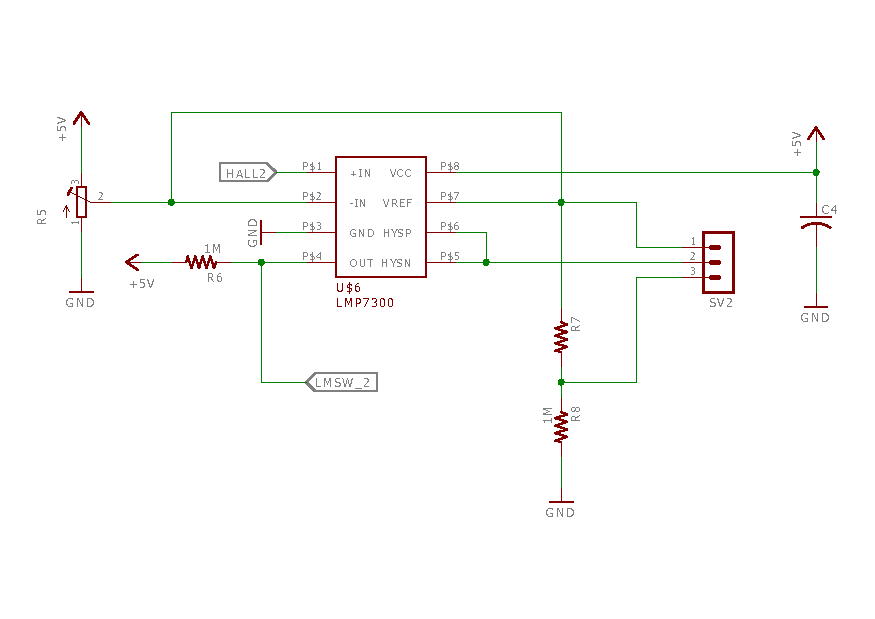
\includegraphics[trim = 0mm 15mm 0mm 15mm]{img/diagram1.pdf}
%trim = izquierda abajo derecha arriba [scale=0.5,trim = 40mm 30mm 110mm 15mm, clip]
\caption{Diagrama Esquem\'{a}tico }
\label{fig:EsqTilt}
\end{figure} 

La tarjeta electronica se dise\~{n}\'{o} usando el programa EAGLE\textsuperscript{\textregistered}, figura ~\ref{fig:CircuitoImp}, integrando el dise\~{n}o mec\'{a}nico del prototipo en el dise\~{n}o electr\'{o}nico para darle una doble funcionalidad a la placa al cuidar la distribuci\'{o}n de los componentes colocando los sensores en la posici\'{o}n necesaria para medir los 90$^\circ$ efectivos de movimiento angular.

\begin{figure}[H]
\centering 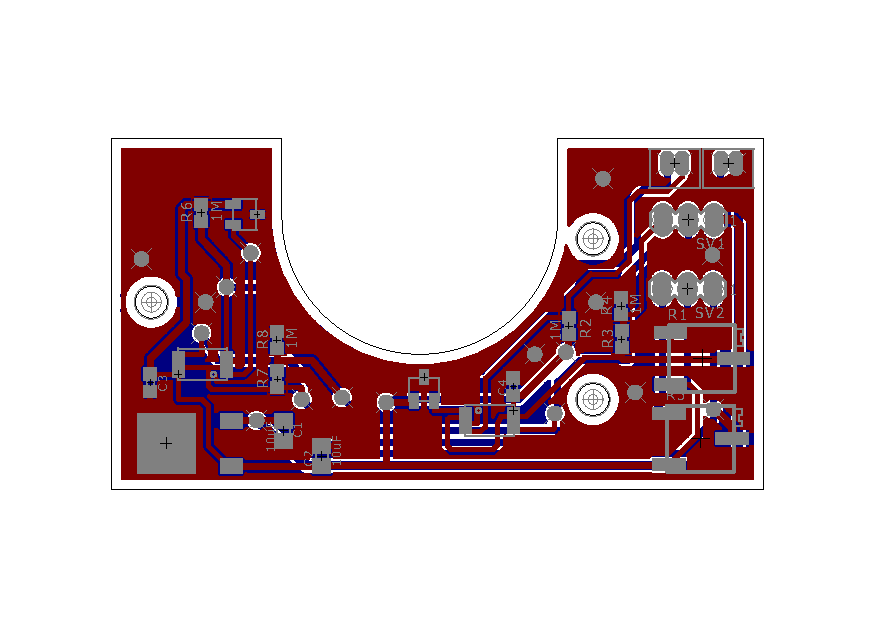
\includegraphics[scale=0.75,trim = 0mm 25mm 0mm 20mm]{img/LimitSW_Tilt_DW_UP.pdf}
%trim = izquierda abajo derecha arriba [scale=0.5,trim = 40mm 30mm 110mm 15mm, clip]
\caption{Dise\~{n}o del Circuito Impreso}
\label{fig:CircuitoImp}
\end{figure} 

Se usaron elementos de montaje superficial para reducir al m\'{a}ximo el tama\~{n}o y el peso del sensor. La forma de placa se ajusta perfectamente para ser montado en el soporte de la c\'{a}mara y la dispoci\'{o}n de los conectores se eligi\'{o} con cuidado para minimizar el uso de cablel El prototipo terminado se muestra en la imagen ~\ref{fig:SenTilt}.

\begin{figure}[H]
\centering 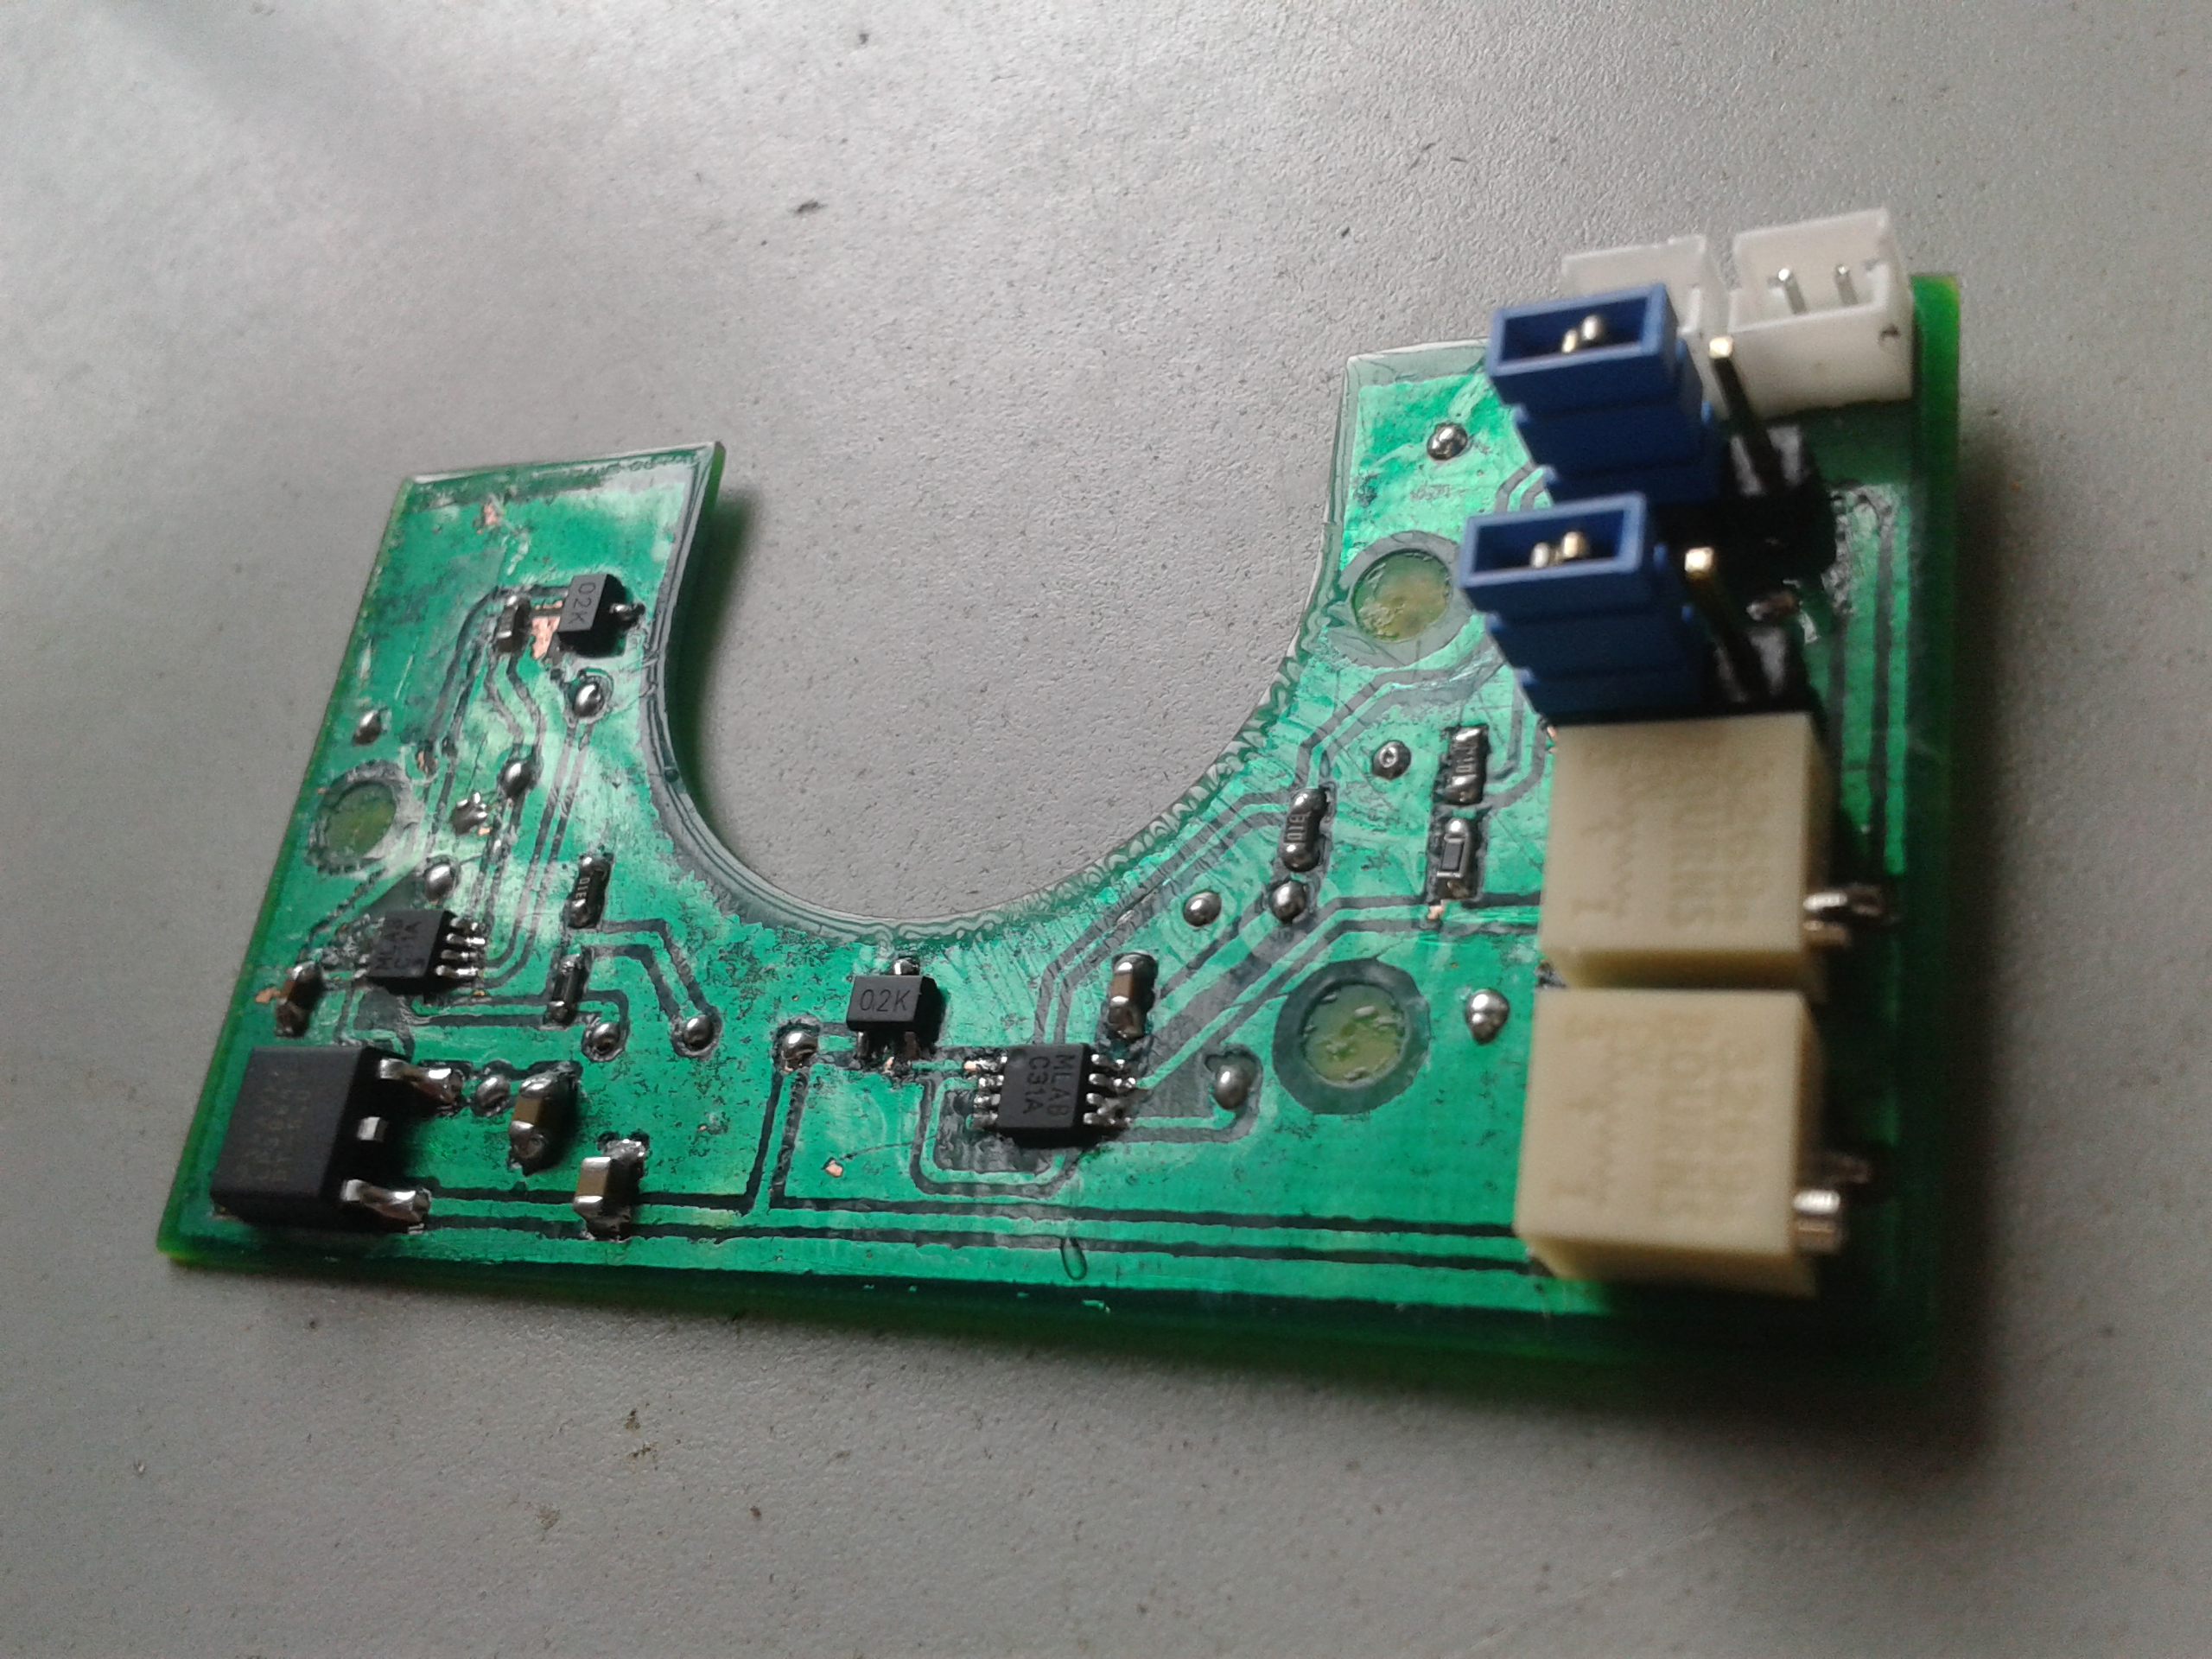
\includegraphics[scale=0.093]{img/SenTilt.jpg}
\caption{Sensor de l\'{i}mite dise\~{n}ado}
\label{fig:SenTilt}
\end{figure} 


Adem\'{a}s de indicar los limites f\'{i}sicos los sensores tienen otra funci\'{o}n importante, la cual es establecer la posici\'{o}n "Home" del sistema, es decir, una ubicaci\'{o}n conocida y fija en el eje de coordenadas del sistema que indique la posici\'{o}n cero para cada eje. La figura ~\ref{fig:HomePos} muestra la posici\'{o}n de los ejes seleccionada para ser la posici\'{o}n cero o "home" del gimbal. 

\begin{figure}[H]
\centering 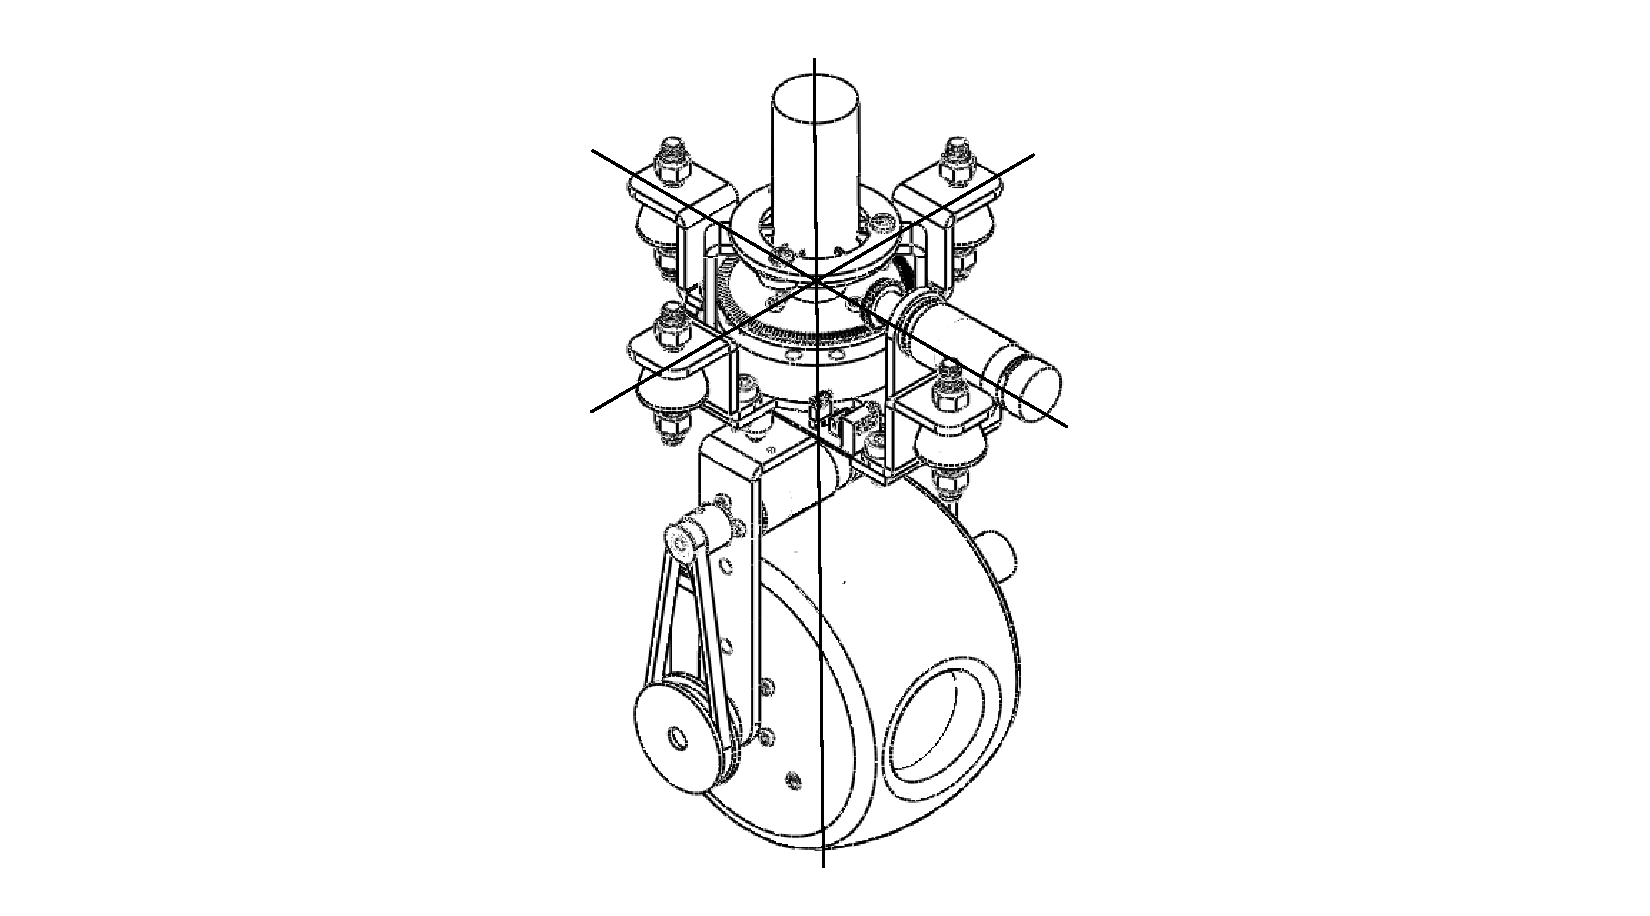
\includegraphics[scale=0.5,trim = 40mm 10mm 40mm 5mm]{img/HomePos.pdf}
%trim = izquierda abajo derecha arriba [scale=0.5,trim = 40mm 30mm 110mm 15mm, clip]
\caption{Posici\'{o}n inicial "Home"}
\label{fig:HomePos}
\end{figure}

Al igual que para el eslab\'{o}n interno se dise\~{n}\'{o} un sensor para el eslab\'{o}n externo. Para este sensor se us\'{o} el mismo sensor radiom\'{e}trico de efecto Hall y el mismo circuito de acondicionamiento. podemos ver el dise\~{n}o de la placa en la figura ~\ref{fig:CircuitoImpPan}.

\begin{figure}[H]
\centering 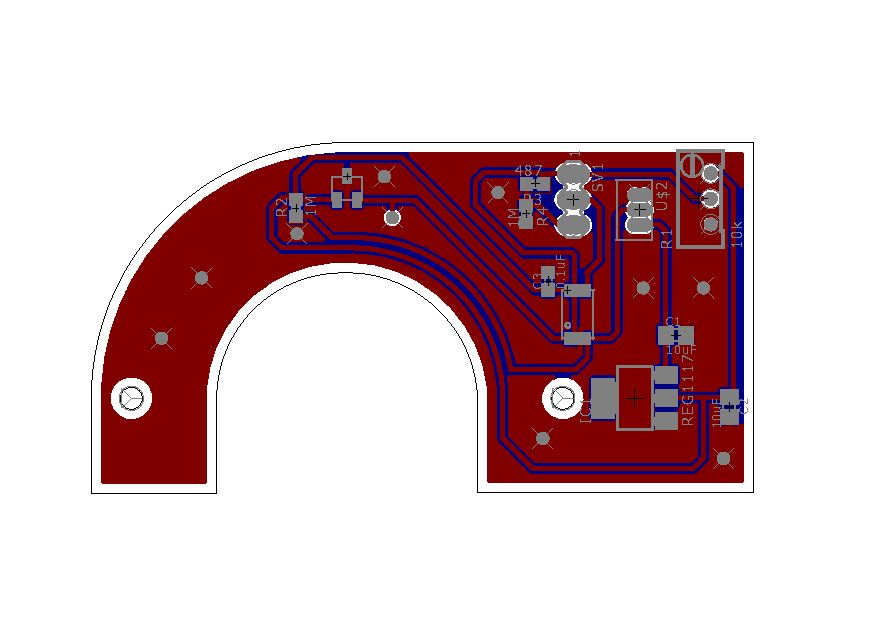
\includegraphics[scale=0.7,trim = 0mm 25mm 0mm 20mm]{img/LimitSW_Pan.pdf}
%trim = izquierda abajo derecha arriba [scale=0.5,trim = 40mm 30mm 110mm 15mm, clip]
\caption{Dise\~{n}o del Circuito Impreso del Sensor de Pan}
\label{fig:CircuitoImpPan}
\end{figure}

Como en el dise\~{n}o anterior se tom\'{o} en cuenta la mec\'{a}nica del gimbal para dise\~{n}ar la electr\'{o}nica. La figura ~\ref{fig:SenPan}, muestra el sensor terminado montado en el la base del gimbal y podemos apreciar el actuador magn\'{e}tico que activar\'{a} el sensor. 

\begin{figure}[H]
\centering 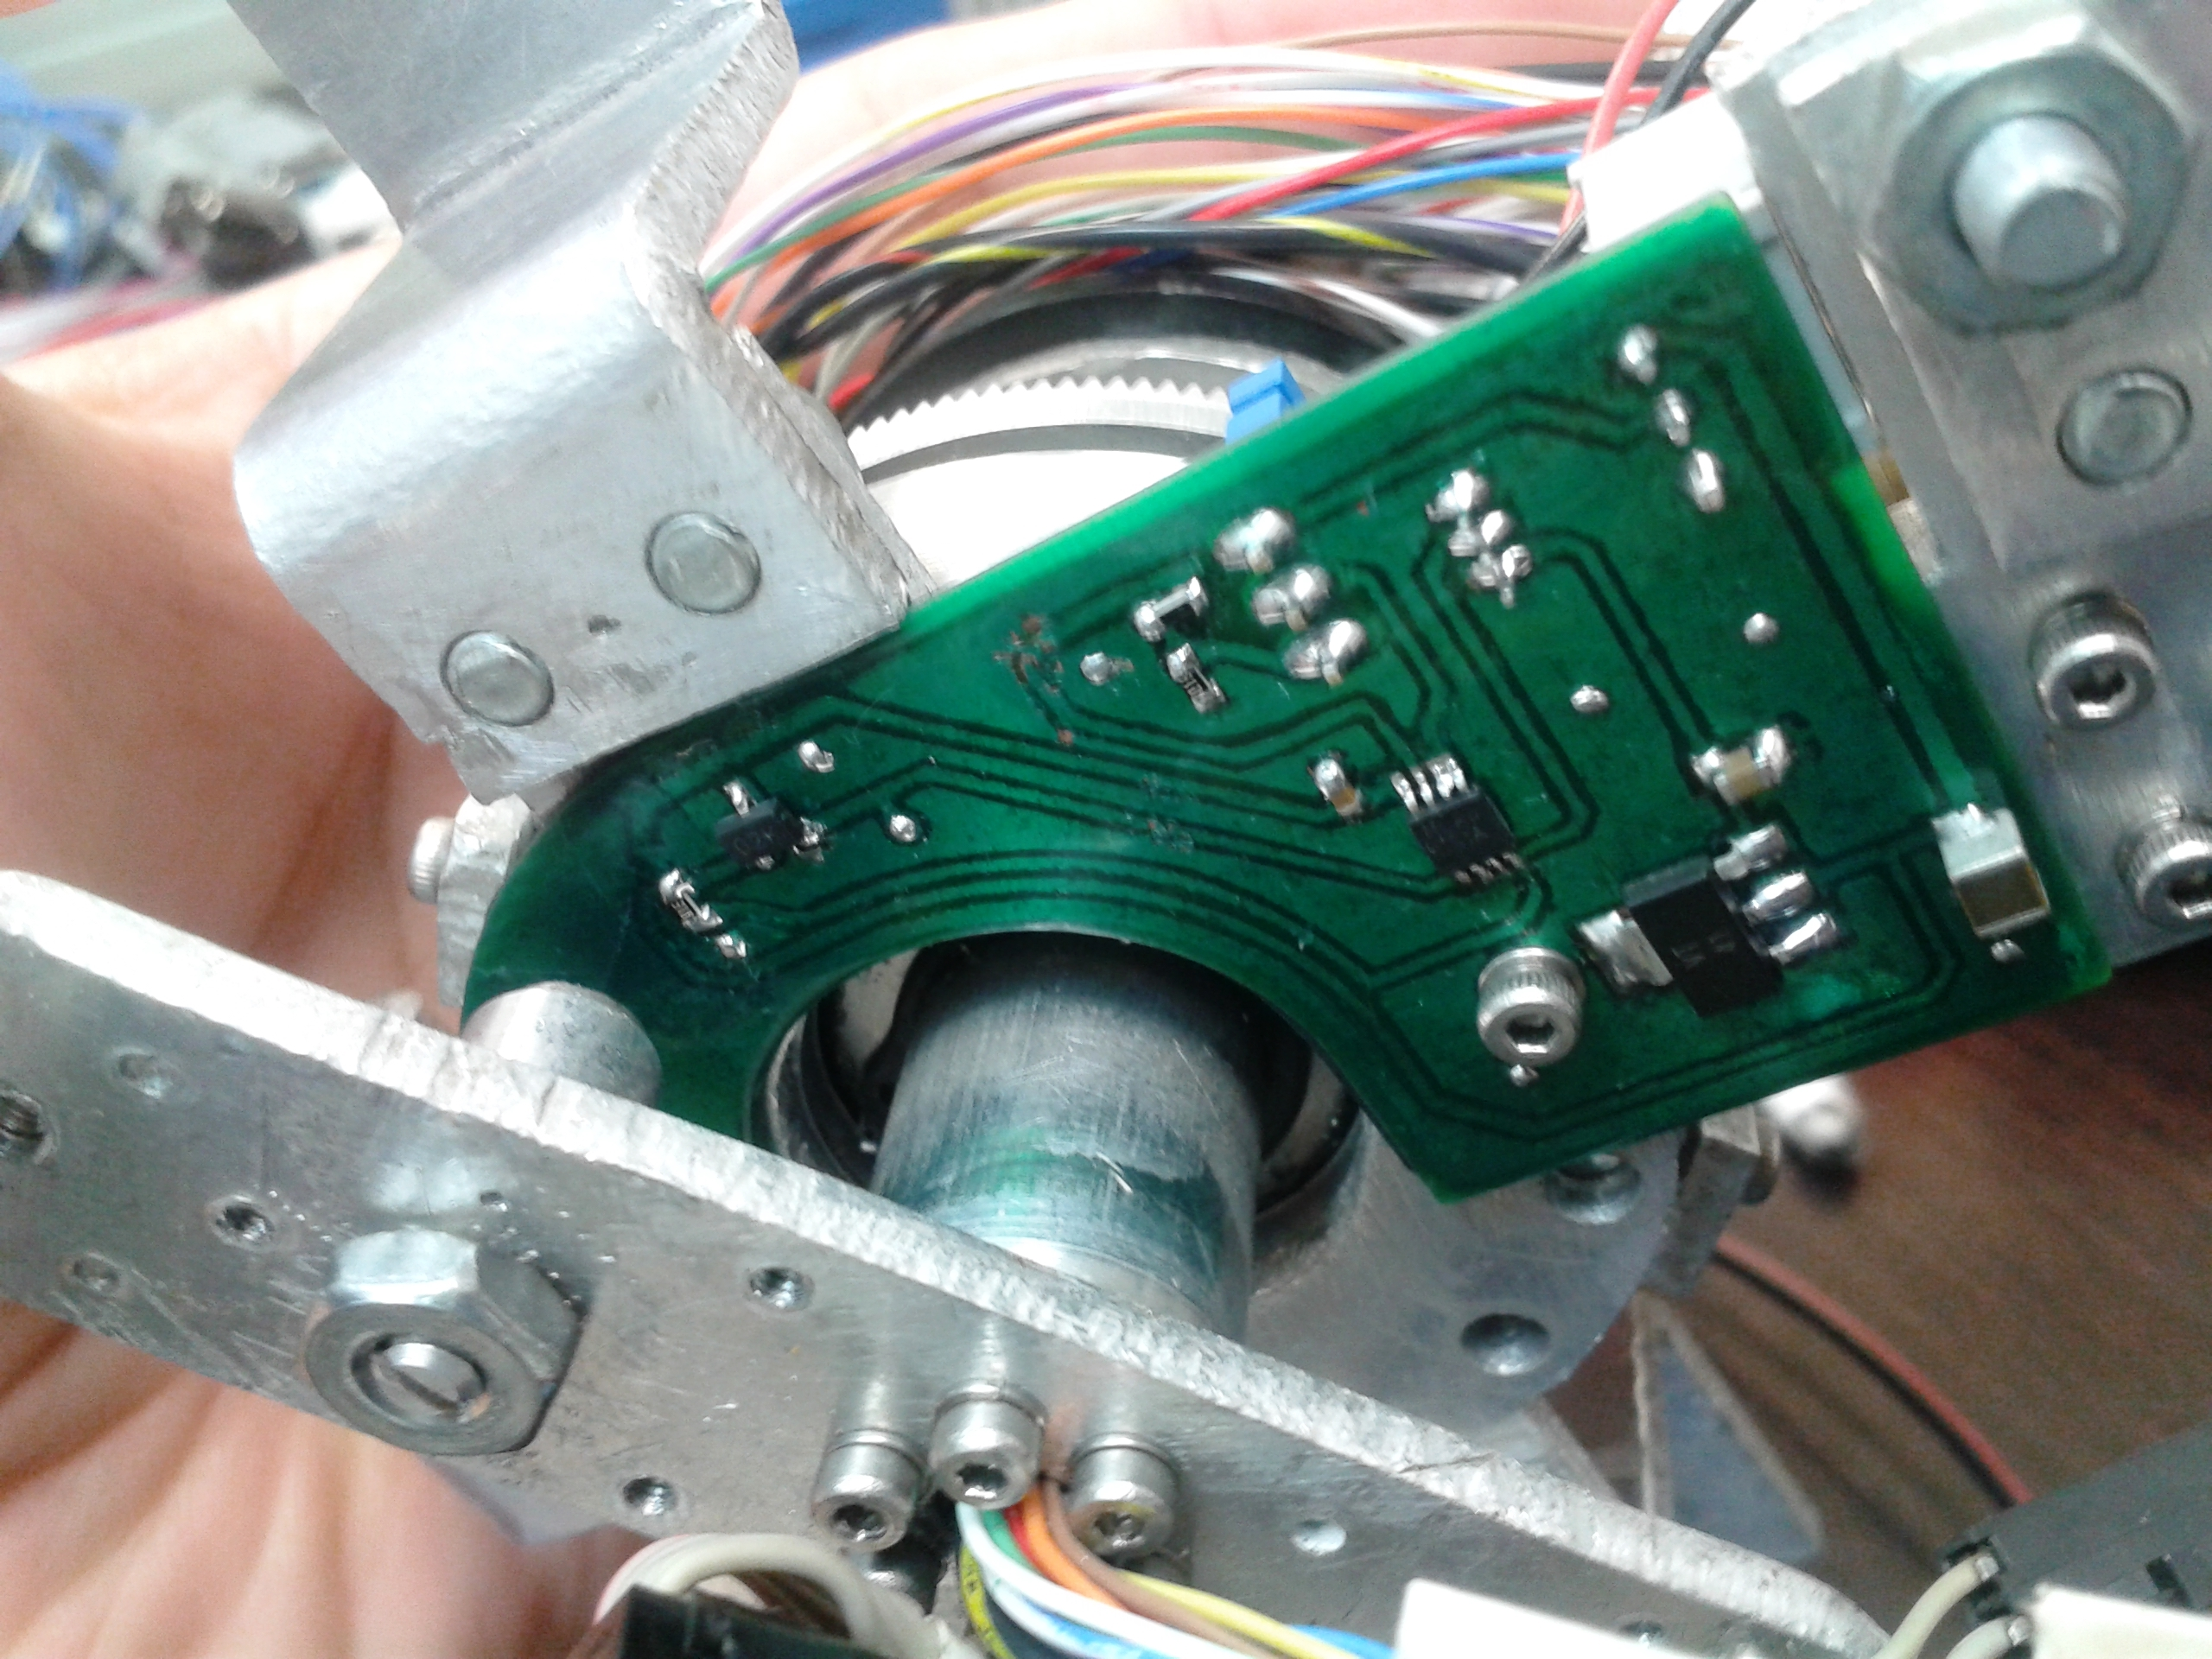
\includegraphics[scale=0.093]{img/SenPan.jpg}
\caption{Sensor de l\'{i}mite Dise\~{n}ado Montado en el Prototipo}
\label{fig:SenPan}
\end{figure}

  
\section{Mec\'anica}

\subsection{Estructura Principal}

La estructura mec\'{a}nica del prototipo consta principalmente de tres partes, la base, la cual permite el montaje del sistema en la aeronave, el eslab\'{o}n externo, el cual permite el movimiento en acimut del sensor  y finalmente el eslab\'{o}n interno el cual permite el movimiento en tilt del sensor. El material utilizado es aluminio 6160, el cual es una aleaci\'{o}n de aluminio endurecido que contiene como principales elementos aluminio, magnesio y silicio.  Tiene buenas propiedades mec\'{a}nicas y es usado generalmente para la construcci\'{o}n de estructuras de aeronaves como las alas y el fuselaje de aviones comerciales y de uso militar \cite{28}. 

La base tiene la funci\'{o}n de fijar el sistema en la plataforma a\'{e}rea, podemos observar a detalle el dise\~{n}o de la base en la figura ~\ref{fig:Base}, esta permite la fijaci\'{o}n del prototipo por medio de cuatro amortiguadores vibratorios que reducen el efecto de las vibraciones sobre el sistema, tambi\'{e}n tiene el motor y la transmici\'{o}n para mover el eslab\'{o}n externo. Para poder transmitir las se\~{n}ales se us\'{o} un slip ring para permitir una rotaci\'{o}n de 360 grados entre la base y el eslab\'{o}n externo.

\begin{figure}[H]
\centering 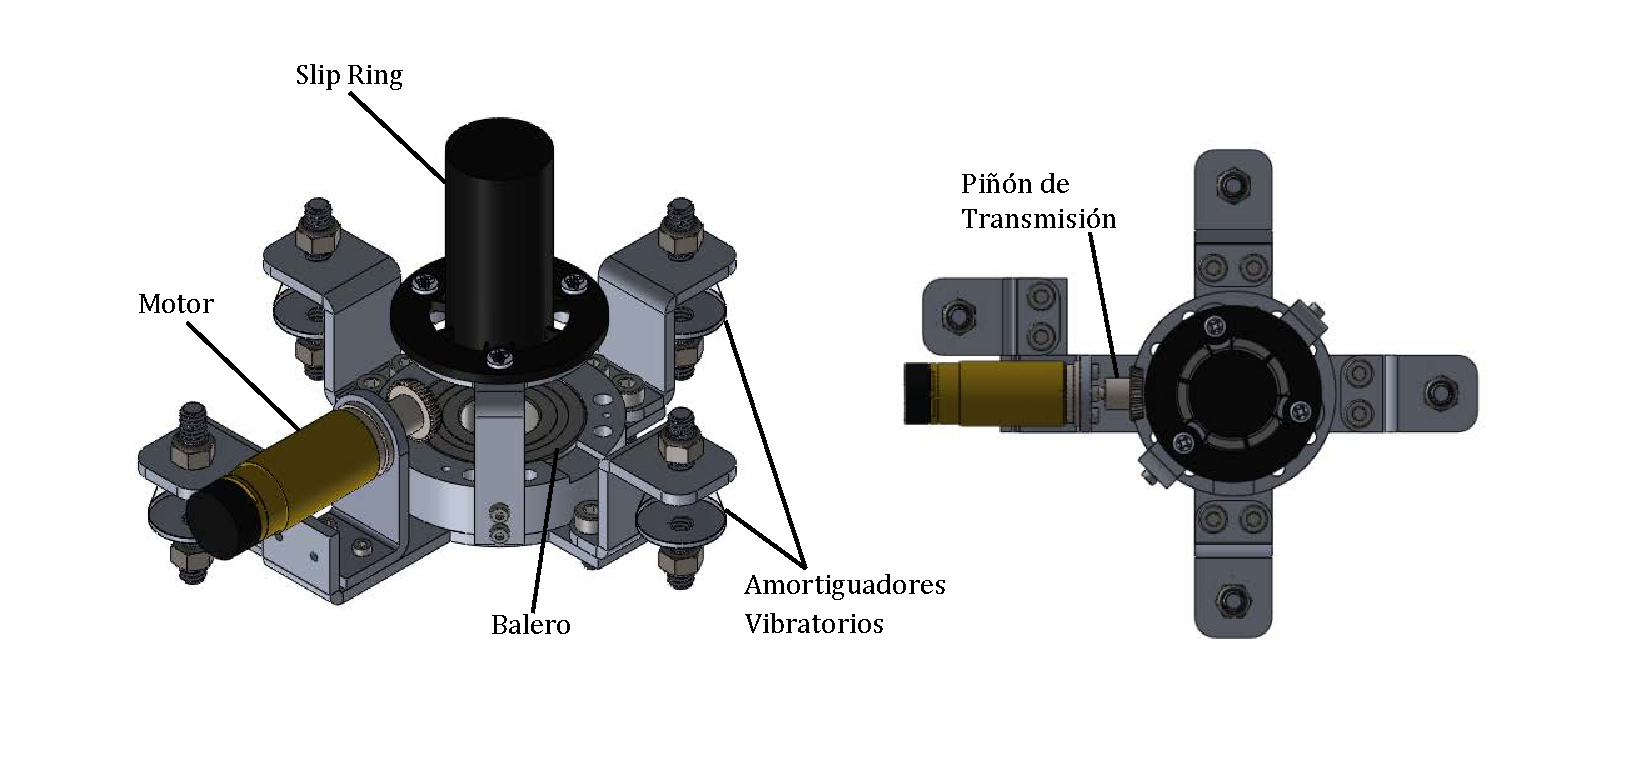
\includegraphics[scale=0.55,trim = 30mm 20mm 30mm 5mm]{img/BaseGimbal.pdf}
%trim = izquierda abajo derecha arriba [scale=0.5,trim = 40mm 30mm 110mm 15mm, clip]
\caption{Detalle de la Estructura de la Base y Montaje del Gimbal}
\label{fig:Base}
\end{figure}

La estructura del eslab\'{o}n externo se muestra en la figura ~\ref{fig:Pan}, en esta imagen podemos observar que consta de un eje al cual se transmite el movimiento a trav\'{e}s de un sistema de corona-pi\~{n}on a la estructura en forma de u que sostendr\'{a} al eslab\'{o}n interno. Este eje esta hueco para que los cables que transmiten las se\~{n}ales desde y hacia la tarjeta principal de control puedan llegar a la tarjeta de control de tilt, estas se\~{n}ales pasan por un dispositivo slip ring tal como se mencion\'{o} anteriormente para permitir un giro completo entre la base y el eslab\'{o}n externo. En esta estructura esta montado el motor que mueve el eslab\'{o}n interno por medio de una transmisi\'{o}n tipo banda. Para poder transmitir las se\~{n}ales hasta la tarjeta de control en tilt, se instal\'{o} un segundo slip ring entre el eslab\'{o}n externo y el interno que tambi\'{e}n podemos apreciar en la figura ~\ref{fig:Pan}, esto permite que el eslab\'{o}n interno pueda realizar giros completos y elimina las restricciones provocadas por los cables. Hay un magneto montado en el eslab\'{o}n externo que sirve como actuador al sensor de l\'{i}mite el cual funciona para calibraci\'{o}n del encoder para medir el \'{a}ngulo entre la base y el eslab\'{o}n externo. 


\begin{figure}[H]
\centering 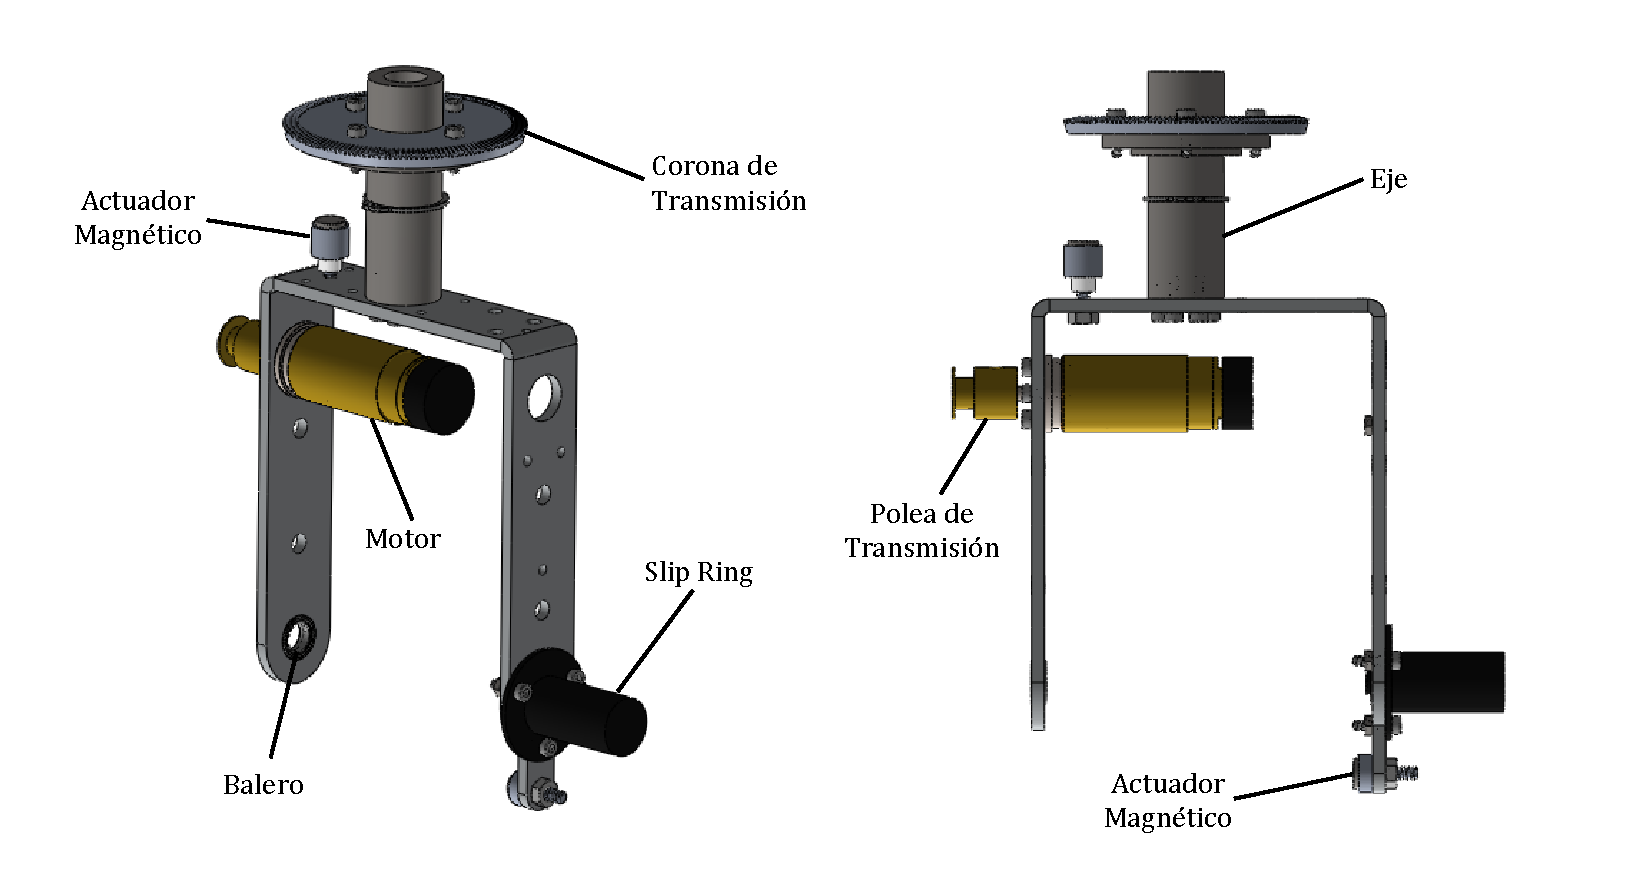
\includegraphics[scale=0.53,trim = 30mm 5mm 30mm 10mm]{img/BasePan.pdf}
%trim = izquierda abajo derecha arriba 
\caption{Detalle de la Estructura del Eslab\'{o}n Externo (Pan)}
\label{fig:Pan}
\end{figure}

La estructura principal del eslab\'{o}n interno se muestra en la figura ~\ref{fig:Tilt}. Este consta de dos ejes de aluminio 6160 y un soporte para la c\'{a}mara fabricado en fibra de vidrio. La transmisi\'{o}n es por medio de una polea y este arreglo permite girar la c\'{a}mara sobre el eje \textit{y} y el montaje de todos los elementos necesarios para el funcionamiento del sistema, es decir, la c\'{a}mara, la central inercial y la tarjeta de control. 


\begin{figure}[H]
\centering 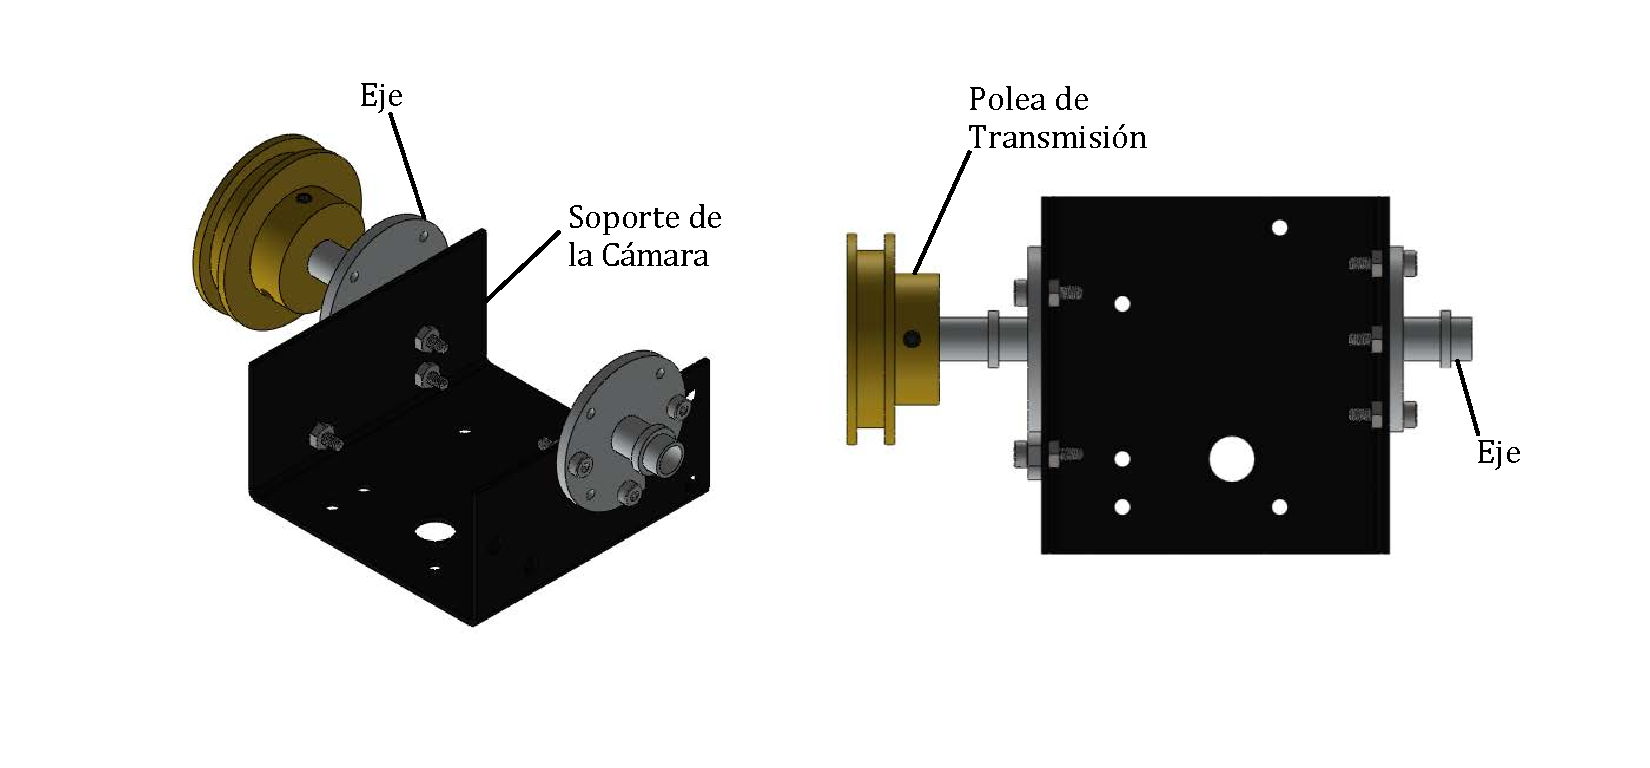
\includegraphics[scale=0.47,trim = 30mm 25mm 20mm 5mm]{img/BaseTilt.pdf}
%trim = izquierda abajo derecha arriba 
\caption{Detalle de la Estructura del Eslab\'{o}n Interno (Tilt)}
\label{fig:Tilt}
\end{figure} 


\section{Programaci\'{o}n}\label{sec:Programacion}

\subsection{Introducci\'{o}n}

\textit{MPLAB\textsuperscript{\textregistered} Device Blocks for Simulink\textsuperscript{\textregistered}} es una tecnolog\'{i}a desarrollada por la empresa Microchip\textsuperscript{\textregistered} que consiste en un juego de bloques que se integra con el ambiente de MATLAB\textsuperscript{\textregistered}/Simulink\textsuperscript{\textregistered} para extender sus capacidades y funciones, los bloques a\~{n}adidos permiten configurar f\'{a}cilmente alrededor de 200 diferentes microcontroladores Microchip \textsuperscript{\textregistered} de las familias dsPIC\textsuperscript{\textregistered}30 y dsPIC\textsuperscript{\textregistered}33. Adicionalmente a los bloques, el \textit{MPLAB\textsuperscript{\textregistered} Device Blocks for Simulink\textsuperscript{\textregistered}} a\~{n}ade codigos a MATLAB que permite programar el microcontrolador y conectarlo a trav\'{e}s  de un puerto serial para analizar los datos. Si bien Simulink y MATLAB son capaces de generar c\'{o}digo C, este paquete adicional permite generar un c\'{o}digo C compatible con el microcontrolador, las tareas que realiza durante el proceso de generaci\'{o}n del c\'{o}digo son las siguientes:    

\begin{itemize}
    \item A\~{n}adir el c\'{o}digo necesario para la configuraci\'{o}n del microcontrolador especifico.
    \item A\~{n}adir el c\'{o}digo necesario para configurar los perif\'{e}ricos usados.
    \item A\~{n}adir el c\'{o}digo del gestionador de tareas.
    \item Compilar el c\'{o}digo global generado para obtener un archivo binario listo para grabar (.cof,
.hex, o .elf).
\end{itemize}

Adicionalmente, crea un proyecto MPLAB X IDE\footnote{Software de programaci\'{o}n para desarrollar aplicaciones para microcontroladores y controladores digitales de se\~{n}ales Microchip\textsuperscript{\textregistered}. Es llamado in Entorno de Desarrollo Integrado (IDE), ya que provee un \'{u}nico entorno integrado para desarrollar c\'{o}digo para microcontroladores embarcados} en donde podemos ver el c\'{o}digo generado.


\subsection{Programaci\'{o}n por Bloques}

En la figura ~\ref{fig:ProgDiag} se muestra uno de los algoritmos programados usando el \textit{MPLAB\textsuperscript{\textregistered} Device Blocks for Simulink\textsuperscript{\textregistered}}. El bloque principal es el "Microchip Master" Este bloque corrobora y corrige los par\'{a}metros de Simulink para cumplir con las restricciones de generaci\'{o}n de c\'{o}digo, adem\'{a}s en este bloque se definen los par\'{a}metros esenciales relacionados con el microcontrolador seleccionado. Por defecto, Simulink est\'{a} preconfigurado con un solucionador continuo que permite  la simulaci\'{o}n ya sea para un modelo continuo, discreto o una mezcla de ambos, tiempo continuo y discreto. Para la generaci\'{o}n de c\'{o}digo se requiere que la configuraci\'{o}n de Simulink sea con el uso de un solucionador de tiempo discreto, cuando se coloca un bloque "Microchip Master" las configuraciones del solucionador se hacen autom\'{a}ticamente.  

\begin{figure}[H]
\centering 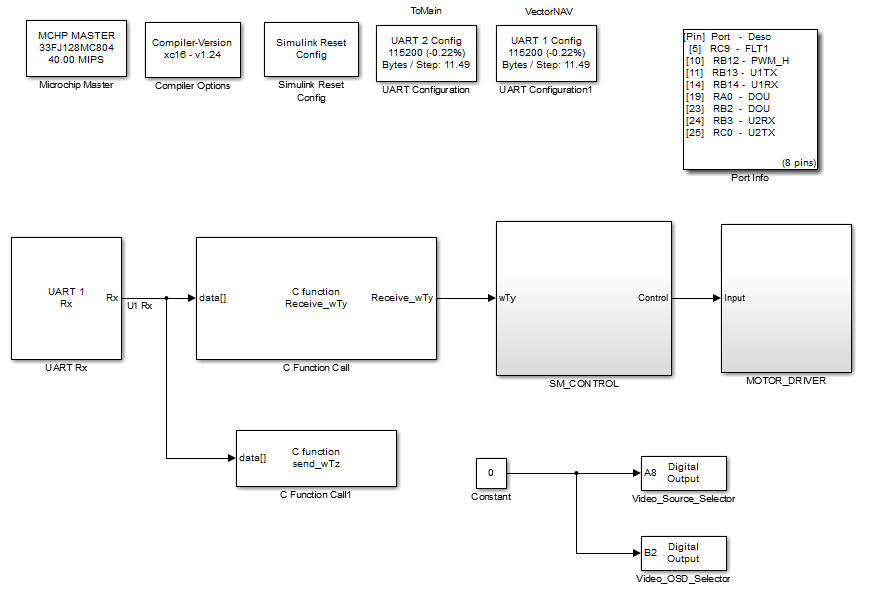
\includegraphics[scale=0.65]{img/DiaProg.png}
\caption{Diagrama de Bloques del Programa del Algoritmo de Estabilizaci\'{o}n}
\label{fig:ProgDiag}
\end{figure}

El bloque \textit{Compiler Option} permite seleccionar el compilador y algunas opciones de compilaci\'{o}n. En este se listan todos los compiladores instalados en el sistema pero no se realiza una prueba de compatibilidad con el dispositivo elegido, por lo que hay que revisar en la documentaci\'{o}n del microcontrolador seleccionado, cual es el compilador compatible. El bloque \textit{Reset Config} revisa que la configuraci\'{o}n de Simulink sea correcta y se usa cuando se trabaja en diferentes computadoras pues permite corregir la ruta de los archivos para la compilaci'{o}n. El bloque \textit{Port info} muestra una relaci\'{o}n de los pines usados en el dispositivo y el perif\'{e}rico al que pertenecen, es muy \'{u}til pues la mayor\'{i}a de los dispositivos soportados tienen pines remapeables por lo que es una ayuda visual para corroborar que la configuraci\'{o}n de los pines corresponde con la capa f\'{i}sica del circuito. El bloque \textit{Digital Output} configura los pines como salidas digitales y permite la escritura en el estado del pin. La entrada del bloque corresponde con la salida digital seleccionada. Un bloque puede configurar \'{u}nicamente un puerto, por ejemplo PORTA o PORTB, pero para el puerto seleccionado pueden configurarse varios pines, cuando se selecciona m\'{a}s de un pin con un bloque, existe la opci\'{o}n para que la actualizaci\'{o}n del estado sea simultanea o de lo contrario la actualizaci\'{o}n ser\'{a} en secuencia. El bloque \textit{UART Configuration} configura el perif\'{e}rico UART elegido: Este bloque permite la configuraci\'{o}n de la velocidad de transmisi\'{o}n  y elegir los pines Rx y Tx. Este bloque permite tambi\'{e}n elegir entre varios tipos de implementaci\'{o}n para la recepci\'{o}n de datos por la comunicaci\'{o}n serial:

 
\begin{itemize}
    \item Solo el buffer\footnote{Es un espacio de memoria, en el que se almacenan datos de manera temporal} interno de 4 bytes.
    \item Buffer Circular.
    \item Modo DMA Ping-Pong.
    \item DMA usando un solo buffer.
\end{itemize}

Las opciones de implementaci\'{o}n DMA solo estan disponibles para los dispositivos que soporten el uso de DMA. Para el modo DMA Ping-Pong, se inicializan dos buffers y se llenan en secuencia. El primer buffer se env\'{i}a hasta que esta completamente lleno. En el modo DMA de un solo buffer, solo se inicializa un buffer y tiene el inconveniente de poder presentar perdida de datos. El bloque \textit{C Function Call} permite incluir c\'{o}digo en lenguaje C dentro del proyecto de Simulink. Estos archivos C ser\'{a}n utilizados para la generaci\'{o}n de c\'{o}digo y permiten la utilizaci\'{o}n de registros e instrucciones especificas del dispositivo. El archivo del c\'{o}digo en C debe declararse en los par\'{a}metros de configuraci\'{o}n de Simulink en el men\'{u} de generaci\'{o}n de c\'{o}digo para a\~{n}adir la ruta del archivo al directorio de Simulink.

En conclusi\'{o}n el \textit{MPLAB\textsuperscript{\textregistered} Device Blocks for Simulink\textsuperscript{\textregistered}}, nos permite traducir nuestro modelo de tiempo discreto en su equivalente binario, implementando tambi\'{e}n c\'{o}digo personalizado para aumentar las funciones de los bloques, gracias a esto el n\'{u}mero de iteraciones entre la simulaci\'{o}n y la implementaci\'{o}n se reducen considerablemente y permite probar el algoritmo desarrollado en el prototipo aprovechando las habilidades en el manejo del entorno Simulink sin necesidad de un extensivo y avanzado conocimiento de microcontroladores.






 %Implementaci�n y Pruebas
%%%simulacion
\chapter{Resultados}

\section{Introducci\'{o}n}

Uno de los objetivos principales de este trabajo consiste en la implementaci\'{o}n pr\'{a}ctica del algoritmo de estabilizaci\'{o}n por modos deslizantes propuesto adem\'{a}s de su comparaci\'{o}n cuantitativa con un algoritmo de control basado en un compensador proporcional-integral el cual es ampliamente usado para el control de este tipo de sistemas. En el cap\'{i}tulo~\ref{sec:ControlChapter} se obtuvieron resultados de simulaci\'{o}n sobre la efectividad del algoritmo de estabilizaci\'{o}n, sin embargo para poder comprobar de una forma m\'{a}s completa el algoritmo es necesaria una implementaci\'{o}n pr\'{a}ctica. Para poder obtener datos sobre el comportamiento del sistema dise\~{n}ado frente a las perturbaciones, se utiliz\'{o} una unidad de medici\'{o}n inercial para la medici\'{o}n de las perturbaciones introducidas en el sistema, este sensor se monta en la base del gimbal y las perturbaciones se realizan de forma manual al manipular el gimbal tratando de ser consistente en los movimientos que se realizan en cada experimento. Las pruebas se realizan de esta manera ya que el dise\~{n}o y construcci\'{o}n de una plataforma de pruebas actuada y con un sistema de control esta fuera del alcance de este trabajo.



\section{Descripci\'{o}n de la Experimentaci\'{o}n}

Para la obtenci\'{o}n de los resultados se realizaron varios experimentos, en los cuales se mont\'{o} una Unidad de Medici\'{o}n Inercial (IMU por sus siglas en ingl\'{e}s) en la base del sistema gimbal, que nos permite medir las perturbaciones inducidas en el sistema, es decir, las velocidades angulares $\omega _{B_y}$ y $\omega _{B_z}$. La IMU utilizada es la MicroStrain 3DM-GX3-25-OEM, que nos permiti\'{o} obtener los datos de la velocidad angular a una frecuencia de 100 Hz en la computadora por medio del software MIP\textsuperscript{\textregistered} Monitor para el control de la IMU, en la figura ~\ref{fig:Prueba} podemos observar la recepci\'{o}n de los datos provenientes de la IMU en la computadora.   

\begin{figure}[H]
\centering
      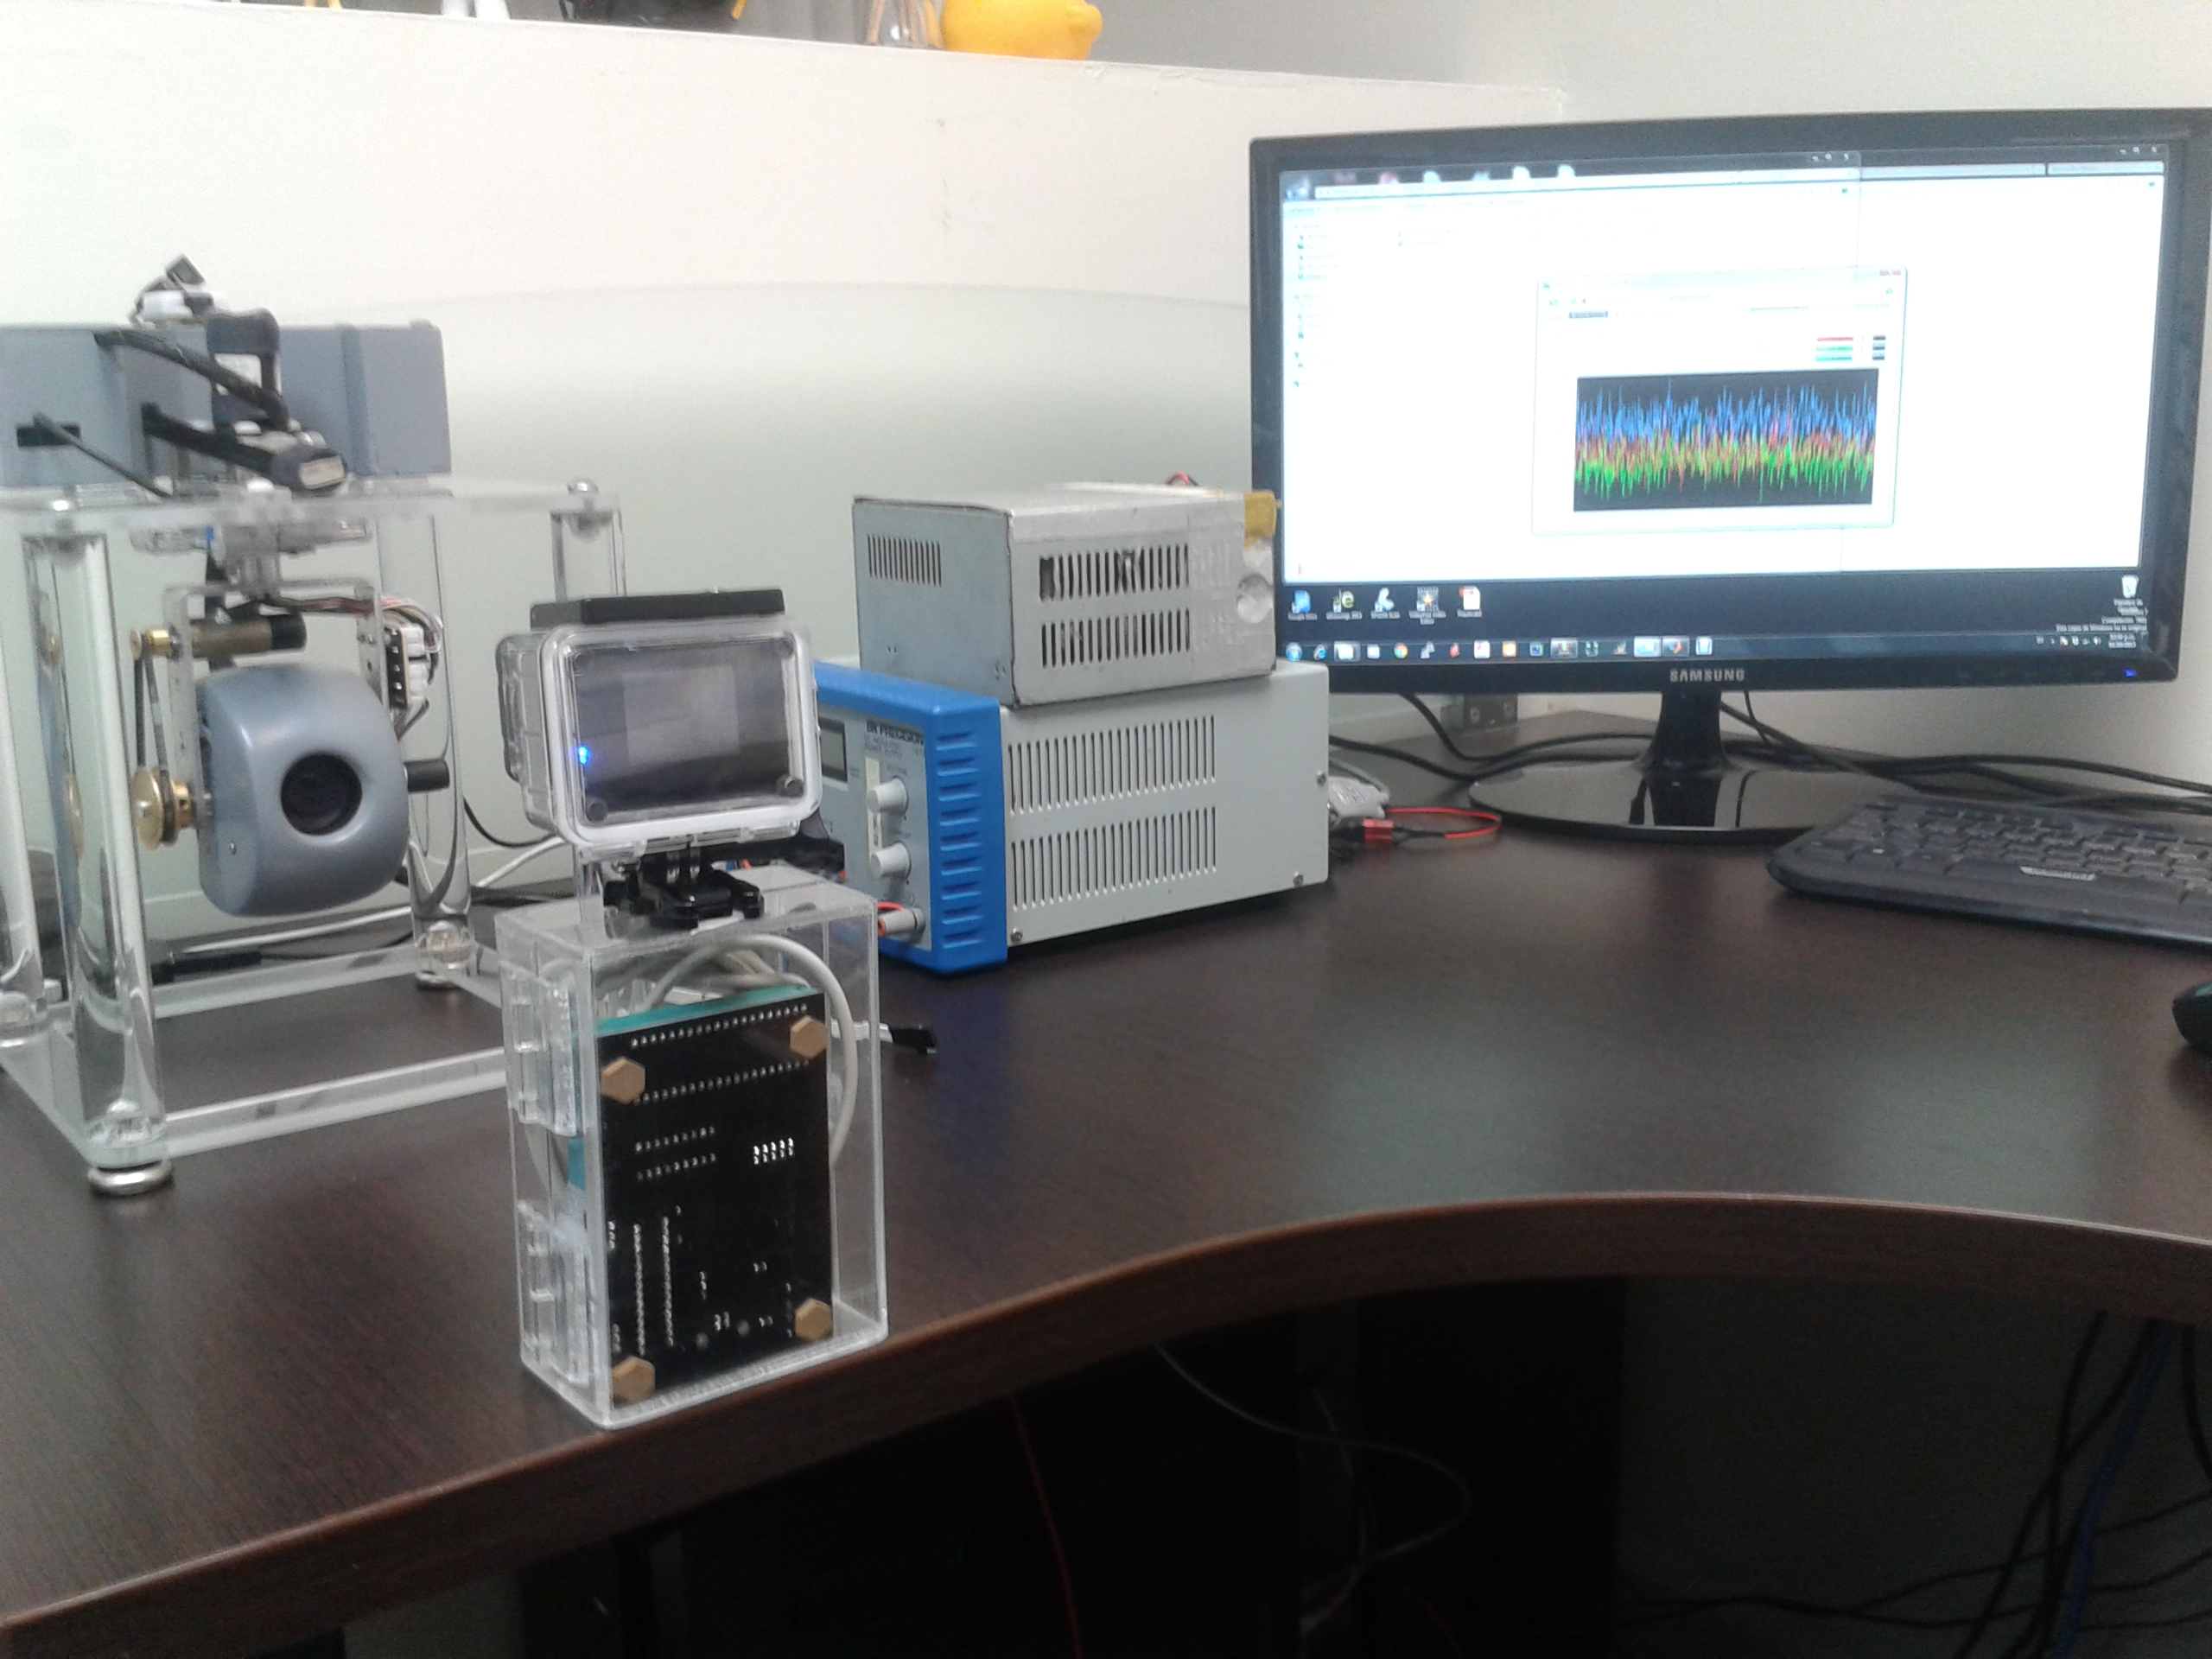
\includegraphics[scale=0.09]{img/Experimentacion.jpg}
      \caption{Pruebas Experimentales}
      \label{fig:Prueba}
\end{figure}

Los datos obtenidos de las velocidades angulares en la base del sistema se guardan en un archivo para poder ser analizados posteriormente y comparados con los datos obtenidos de la IMU montada en el eslab\'{o}n interno del gimbal. El sistema fue perturbado de forma manual enfatizando las perturbaciones en los ejes $y$ y $z$ del sistema, ya que estos son los de mayor inter\'{e}s al ser los ejes actuados. \'{E}sta metodolog\'{i}a se llev\'{o} a cabo para el algoritmo por modos deslizantes y para el compensador PI para poder observar ambas respuestas, a continuaci\'{o}n se presentan los resultados. 

%\begin{figure}[H]
%\centering
%      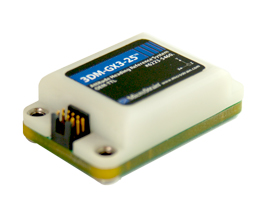
\includegraphics[scale=0.5]{img/MicroStrain.jpg}
%      \caption{Unidad de Medici\'{o}n Inercial MicroStrain}
%      \label{fig:MicroStrain}
%\end{figure}

\section{Resultados Algoritmo Proporcional-Integral}  

En la figura ~\ref{fig:ResPIPer}-a podemos observar la perturbaci\'{o}n ejercida sobre el sistema, mientras que en la figura ~\ref{fig:ResPIPer}-b se muestra la velocidad angular medida en el eslab\'{o}n interno del gimbal, es decir, la respuesta del sistema con el algoritmo del compensador Proporcional-Integral programado en las tarjetas de control. 

\begin{figure}[H]
\centering 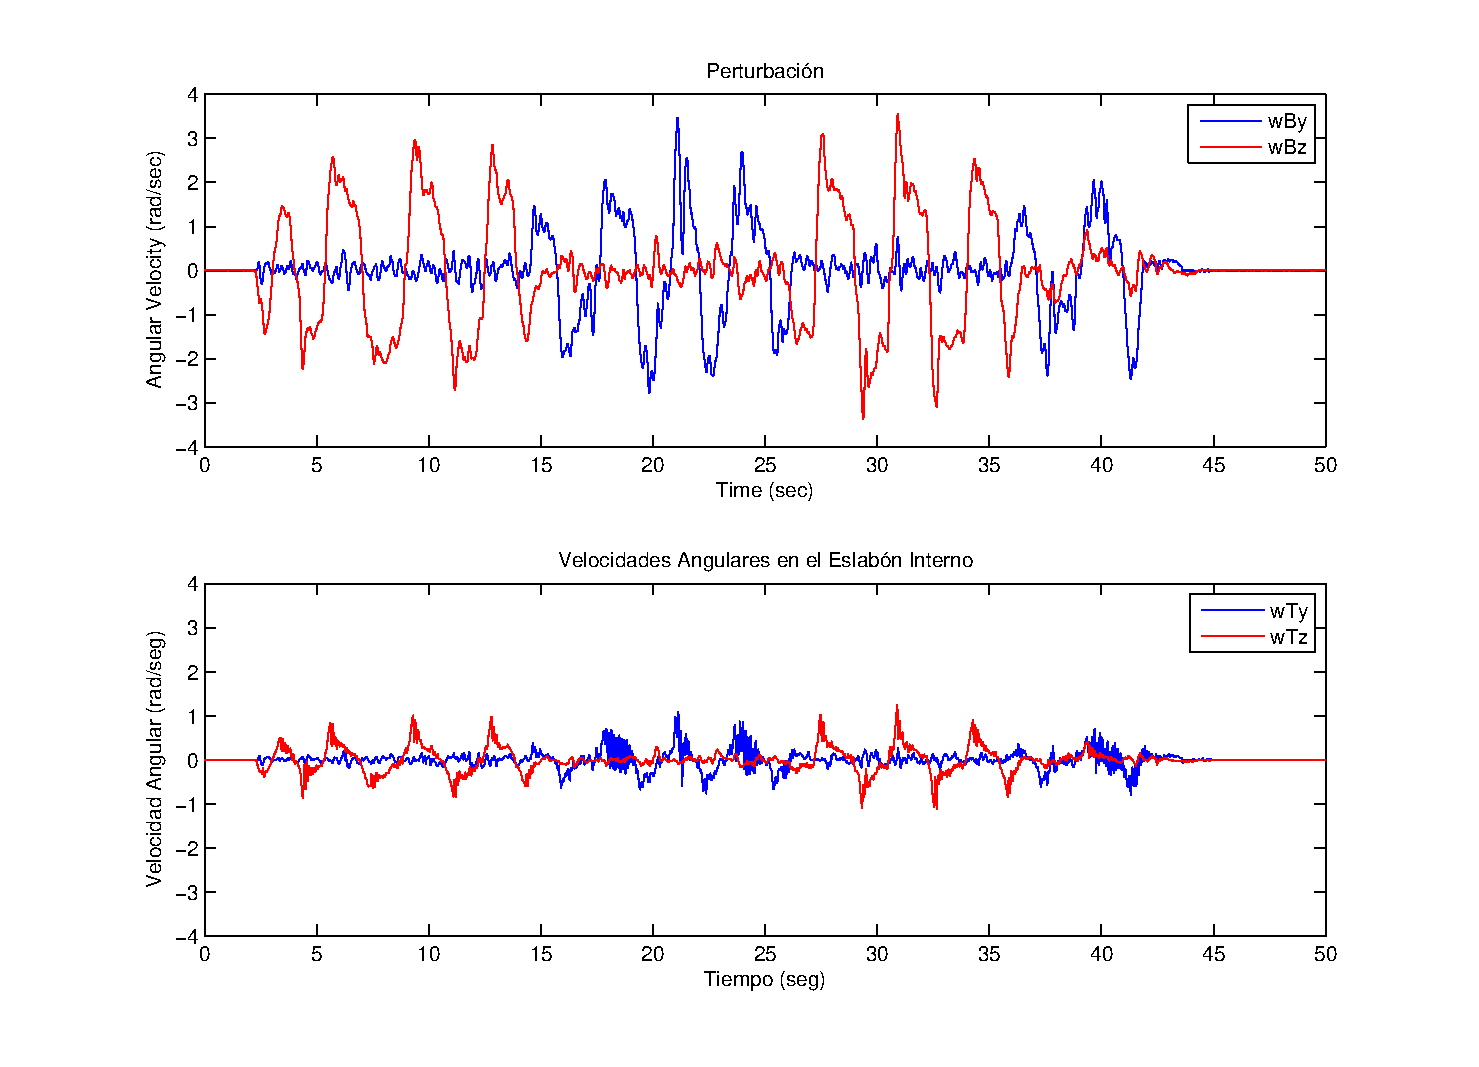
\includegraphics[scale=0.63,trim = 20mm 0mm 20mm 0mm]{img/ResPIPer.eps}
%trim = izquierda abajo derecha arriba [scale=0.5,trim = 40mm 30mm 110mm 15mm, clip]
      \caption{Resultados de la Estabilizaci\'{o}n Proporcional-Integral}
      \label{fig:ResPIPer}
\end{figure}

Podemos observar que el algoritmo compensa en gran medida las perturbaciones, sin embargo la estabilizaci\'{o}n no es perfecta, esto puede deberse a varios factores , por ejemplo la sintonizaci\'{o}n de las constantes de control $K_p$ y $K_i$ podr\'{i}a no ser la \'{o}ptima, ecuaciones ~\ref{eq:ContPIElev} y ~\ref{eq:ContPICross}, adem\'{a}s el algoritmo de estabilizaci\'{o}n se ejecuta en la tarjeta de control a una frecuencia de 40 Hz la cual es posible que no sea suficiente para eliminar las perturbaciones aplicadas.  

En la figura ~\ref{fig:ResPIVs}-a se muestra la comparaci\'{o}n entre la perturbaci\'{o}n aplicada en el eje-$y$, $\omega_{B_y}$ y la velocidad angular sobre el eje de elevaci\'{o}n $\omega_{T_y}$. En la figura ~\ref{fig:ResPIVs}-b, se muestra la perturbaci\'{o}n al sistema $\omega_{B_z}$ gr\'{a}ficada junto con la velocidad angular del gimbal en el eje de la elevaci\'{o}n cruzada $\omega_{T_z}$. 

\begin{figure}[H]
\centering 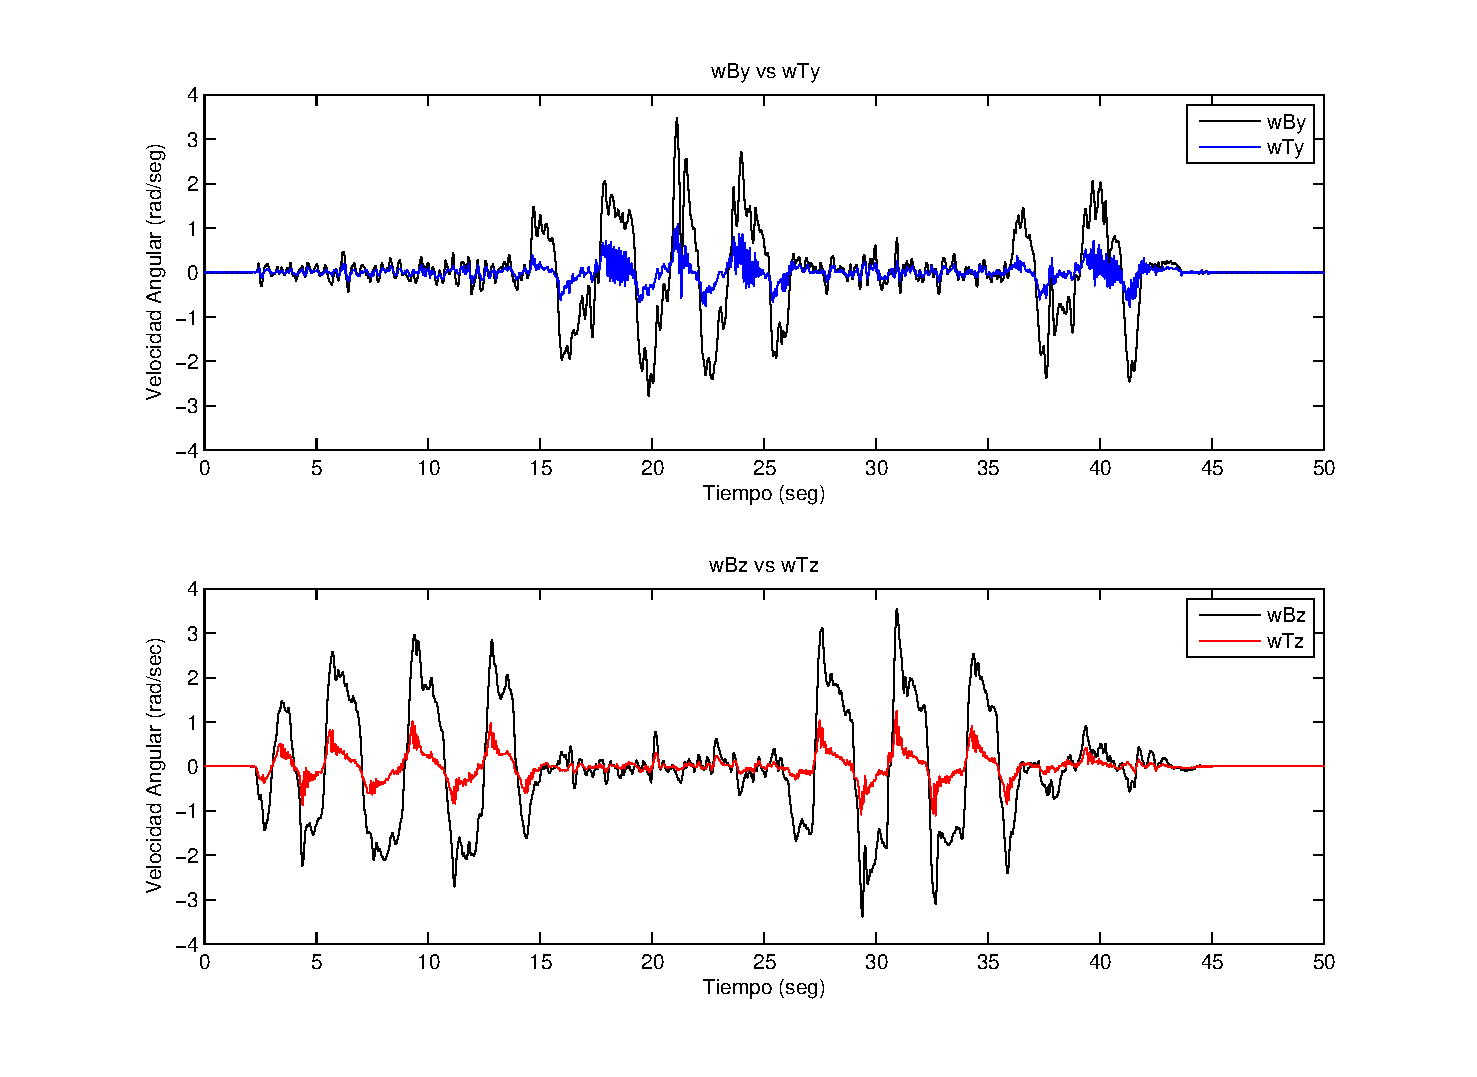
\includegraphics[scale=0.63,trim = 20mm 0mm 20mm 0mm]{img/ResPIVs.eps}
%trim = izquierda abajo derecha arriba [scale=0.5,trim = 40mm 30mm 110mm 15mm, clip]
      \caption{Resultados de la Estabilizaci\'{o}n Proporcional-Integral}
      \label{fig:ResPIVs}
\end{figure}

Estas g\'{a}ficas nos permiten observar m\'{a}s detalladamente el efecto de la estabilizaci\'{o}n sobre los ejes de inter\'{e}s, estas nos muestran la perturbaci\'{o}n ejercida sobre el sistema en contraste con la acci\'{o}n de control. Podemos ver que el algoritmo de control reduce las perturbaciones, logrando en parte el objetivo de estabilizar la l\'{i}nea de vista de la c\'{a}mara montada en el eslab\'{o}n interno del gimbal.

\section{Resultados Algoritmo Por Modos Deslizantes}

En esta secci\'{o}n se exponen los resultados obtenidos de la implementaci\'{o}n del algoritmo de estabilizaci\'{o}n por modos deslizantes en el prototipo construido. De igual forma que para el compensador PI, se perturb\'{o} el sistema de manera manual. En la figura ~\ref{fig:ResSMPer}-a se muestran las gr\'{a}ficas de las perturbaciones medidas por la IMU Microstrain montada en la base del sistema. En la figura ~\ref{fig:ResSMVs}-b se muestra la velocidad angular medida en los ejes de inter\'{e}s de elevaci\'{o}n y elevaci\'{o}n cruzada ante las perturbaciones ejercidas.   

\begin{figure}[H]
\centering 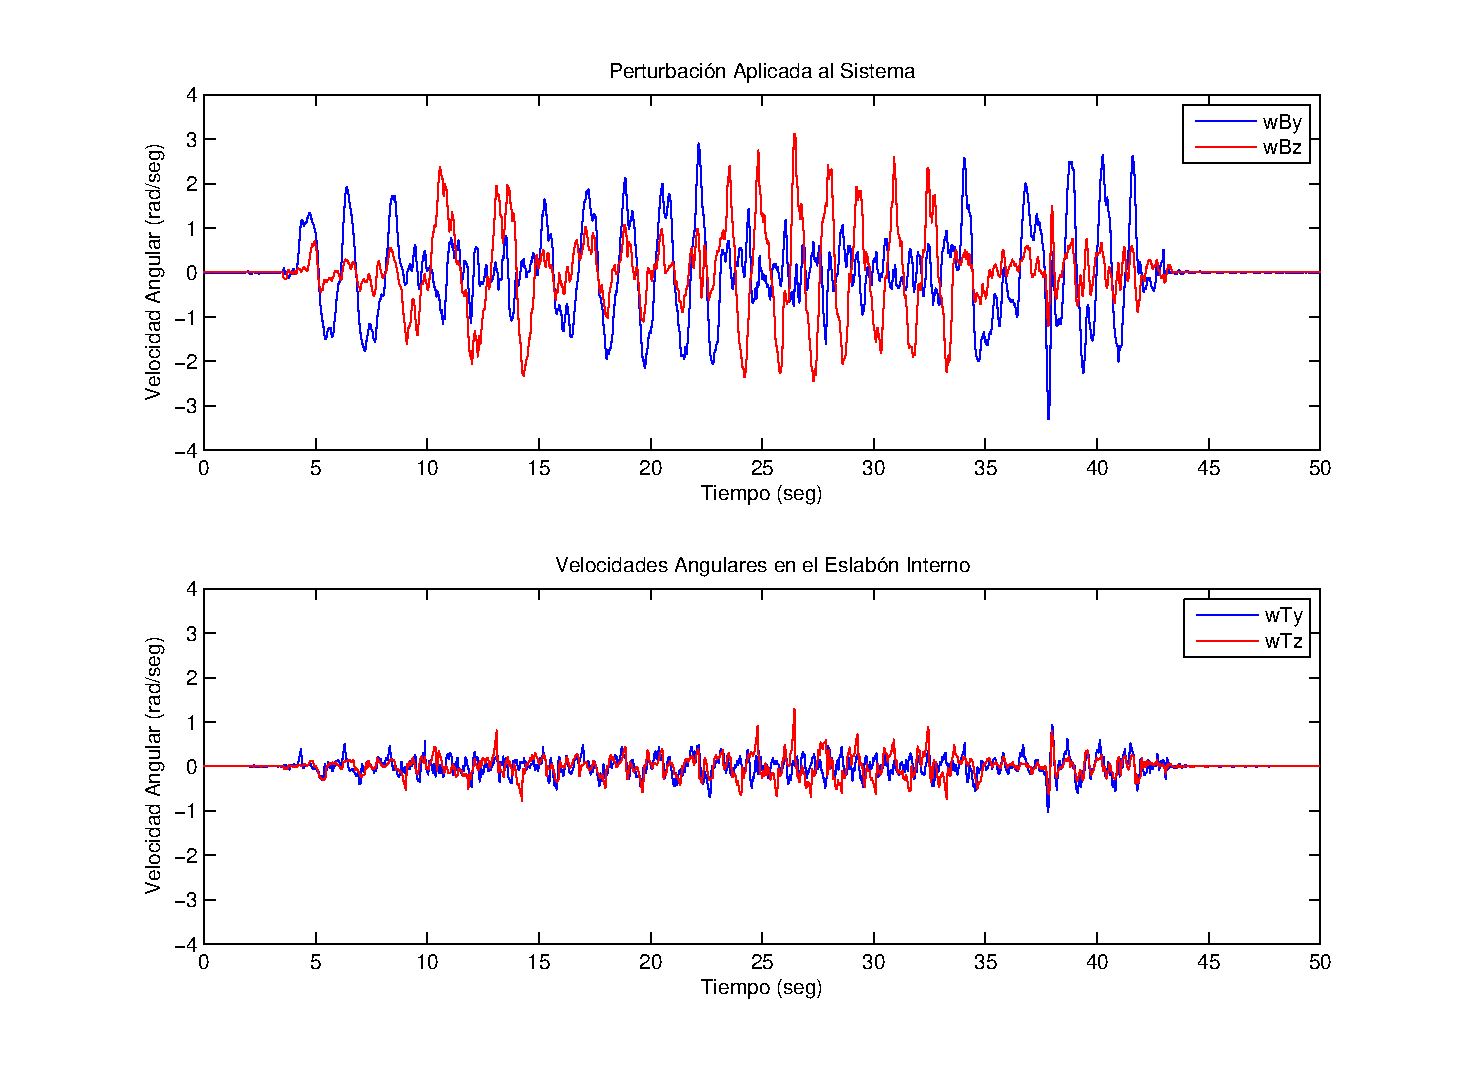
\includegraphics[scale=0.63,trim = 20mm 0mm 20mm 0mm]{img/ResSMPer.eps}
%trim = izquierda abajo derecha arriba [scale=0.5,trim = 40mm 30mm 110mm 15mm, clip]
      \caption{Resultados de la Estabilizaci\'{o}n por Modos deslizantes}
      \label{fig:ResSMPer}
\end{figure}

Es evidente que el control por modos deslizantes tiene un mejor desmpe\~{n}o que el compensador proporcional-integral, pues cancela de una mejor manera las perturbaciones. En la figura ~\ref{fig:ResSMVs}-a se muestra la gr\'{a}fica de la perturbaci\'{o}n en el eje-$y$ contra la velocidad angular medida en el eje de elevaci\'{o}n, mientras que en la figura ~\ref{fig:ResSMVs}-b se muestra la perturbaci\'{o}n en el eje-$z$ graficada junto con la respuesta del sistema en el eje de elevaci\'{o}n cruzada. 

\begin{figure}[H]
\centering 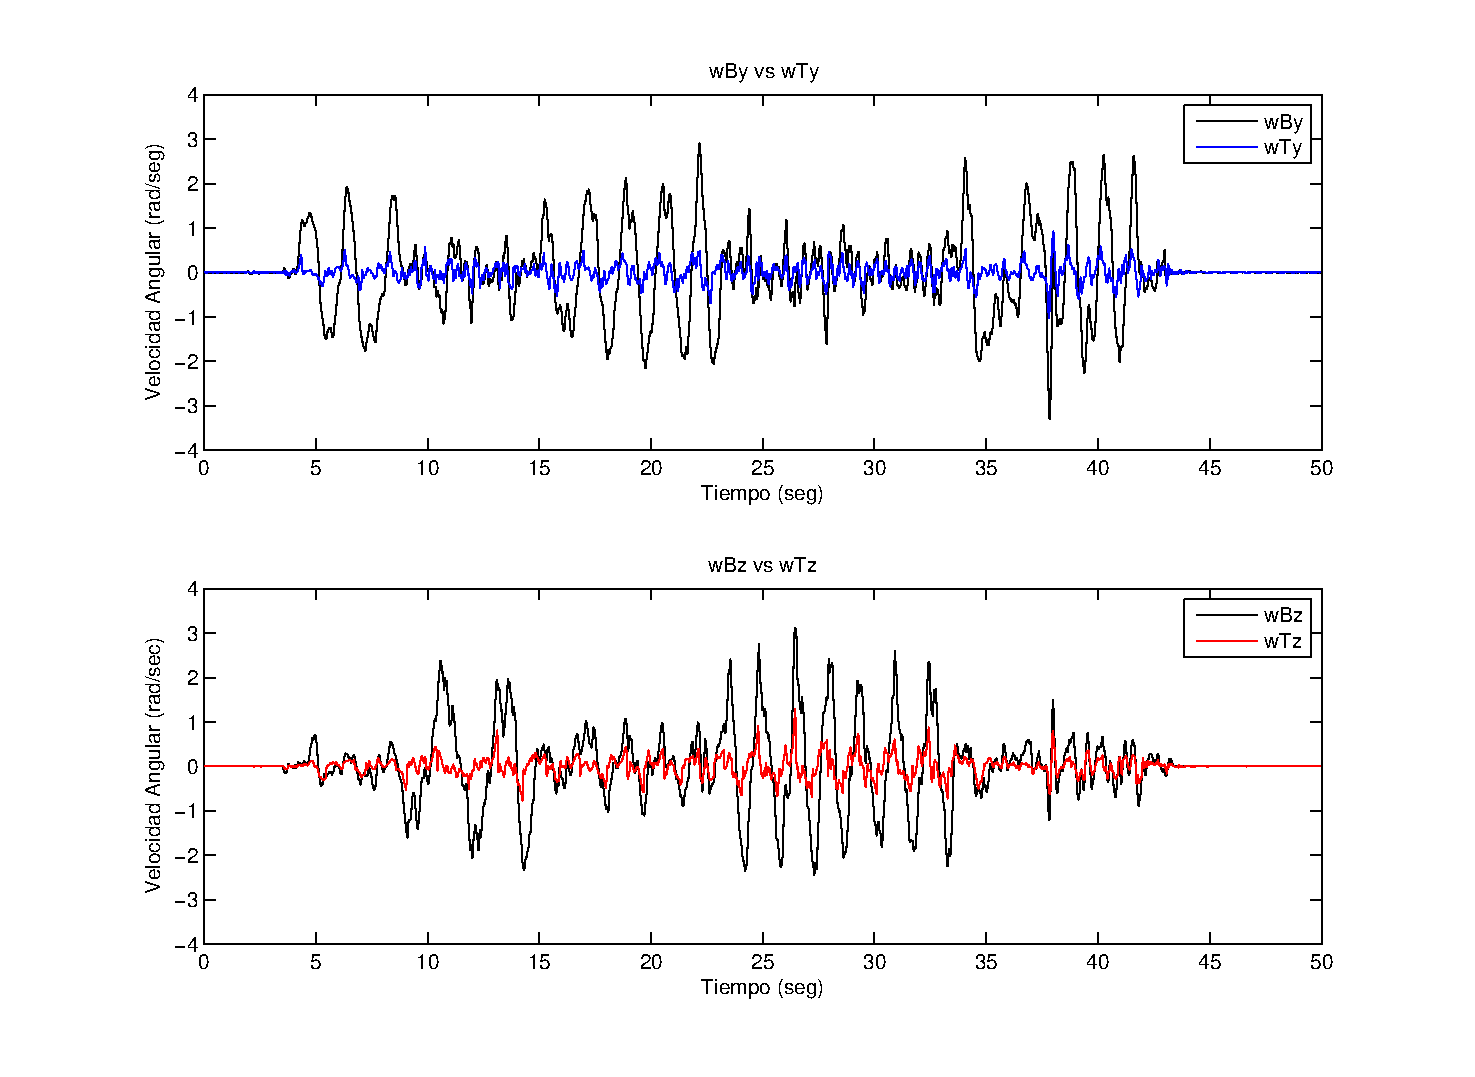
\includegraphics[scale=0.63,trim = 20mm 0mm 20mm 0mm]{img/ResSMVs.eps}
%trim = izquierda abajo derecha arriba [scale=0.5,trim = 40mm 30mm 110mm 15mm, clip]
      \caption{Resultados de la Estabilizaci\'{o}n por Modos deslizantes}
      \label{fig:ResSMVs}
\end{figure}

Haciendo una comparativa entre las perturbaciones y las respuestas de cada algoritmo implementado podemos concluir que el algoritmo de estabilizaci\'{o}n por modos deslizantes tiene un mejor desempe\~{o} que el compensador PI pues su respuesta presenta un menor error en la cancelaci\'{o}n de la perturbaci\'{o}n, es decir, mantiene la velocidad angular en el eje de elevaci\'{o}n y elevaci\'{o}n cruzada m\'{a}s cercanas al cero, adem\'{a}s de haber compensado mejor una perturbaci\'{o}n de una frecuencia ligeramente mayor.   %Resultados
%%%simulacion
\chapter{Conclusiones y Trabajo Futuro}
\section{Conclusiones}

En esta tesis se ha presentado el desarrollo de una plataforma de c\'{a}mara giroestabilizada para un veh\'{i}culo a\'{e}reo no tripulado con el fin de ser usada en misiones de reconocimiento, vigilancia e inteligencia. En resumen, en este trabajo se ha presentado:

\begin{enumerate}[1.]
\item La obtenci\'{o}n de las ecuaciones de movimiento de un sistema gimbal de dos grados de libertad usando el m\'{e}todo de Newton-Euler bajo ciertas consideraciones de simetr\'{i}a en la distribuci\'{o}n de masa con respecto a los ejes principales de inercia.

\item El an\'{a}lisis de las propiedades din\'{a}micas del sistema gimbal en base al modelo desarrollado y las limitaciones del mismo en los puntos singulares cercanos al cono de oclusi\'{o}n.      

\item Se desarroll\'{o} el control para la estabilizaci\'{o}n de la l\'{i}nea de vista basado en la teor\'{i}a del control por modos deslizantes al considerar las perturbaciones generadas por el acoplamiento cruzado y la din\'{a}mica inercial como una sola perturbaci\'{o}n acotada y canales independientes para la elevaci\'{o}n y la elevaci\'{o}n cruzada.

\item Se realiz\'{o} la simulaci\'{o}n del sistema y del control dise\~{n}ado en el entorno Simulink para el an\'{a}lisis de su respuesta ante las perturbaciones de la base.

\item Se present\'{o} la comparaci\'{o}n del algoritmo de estabilizaci\'{o}n dise\~{n}ado con un compensador proporcional-integral com\'{u}nmente usado para el control de este tipo de sistemas y se realizaron simulaciones de ambos algoritmos para obtener datos cuantitativos del desempe\~{n}o del control dise\~{n}ado.

\item Se realiz\'{o} el dise\~{n}o detallado en 3D del prototipo en el programa SolidWorks. Este modelo permiti\'{o} obtener los par\'{a}metros inerciales para la simulaci\'{o}n.

\item Se realiz\'{o} la construcci\'{o}n y programaci\'{o}n del prototipo y se obtuvieron resultados de la implementaci\'{o}n por medio de experimentaci\'{o}n en tierra del algoritmo dise\~{n}ado y del compensador proporcional-integral. 

\end{enumerate}   

Podemos concluir en lo referente al modelado, que si bien el modelo obtenido no coincide perfectamente con el comportamiento del gimbal real, es suficiente para el dise\~{n}o de algoritmos de control. 

Por otro lado se logr\'{o} el objetivo de dise\~{n}ar y construir un prototipo funcional que sirva para desarrollar futuras investigaciones en el Instituto de Investigaci\'{o}n y desarrollo Tecnol\'{o}gico de la Armada de M\'{e}xico (INIDETAM) sobre este tipo de sistemas con el objetivo de que en un futuro se pueda eliminar la dependencia tecnol\'{o}gica nacional que actualmente se tiene para la aplicaci\'{o}n de los sistemas de giroestabilizaci\'{o}n inercial de c\'{a}mara.
\newpage

\section{Trabajo Futuro}

La investigaci\'{o}n desarrollada y documentada en \'{e}sta tesis, provee las bases para la realizaci\'{o}n de posteriores investigaciones y trabajos futuros sobre el sistema gimbal. algunos de los aspectos en los que podr\'{i}a desarrollarse una mejora incluyen:

\begin{enumerate}[1.]
\item En la parte te\'{o}rica del modelado, podr\'{i}a desarrollarse un modelo m\'{a}s aproximado a la situaci\'{o}n real del sistema, en el que se consideren las masas no balanceadas y adem\'{a}s desarrollar el modelo de la cinem\'{a}tica inversa del sistema. Por otra parte, Los problemas relacionados con los puntos singulares como el cono de oclusi\'{o}n descrito en la secci\'{o}n ~\ref{sec:propiedadessist} podr\'{i}an eliminarse al realizar un algoritmo basado en cuaterniones, como en se realiza en \cite{7}.

\item El uso de algoritmos de seguimiento de objetivos es una de las aplicaciones m\'{a}s importantes de este tipo de sistemas, por lo que el siguiente paso l\'{o}gico a seguir en el desarrollo de esta investigaci\'{o}n ser\'{i}a el a\~{n}adir capacidades de seguimiento de objetivo al prototipo. Existen investigaciones interesantes en este campo como en \cite{27} el cual consiste en un sistema de zoom activo que ayuda a mejorar las capacidades del sistema de seguimiento.

\item En el \'{a}rea del control podr\'{i}an desarrollarse m\'{a}s esfuerzos en la s\'{i}ntesis de algoritmos avanzados de control como los tratados en las referencias \cite{15}-\cite{18} adem\'{a}s de la aplicaci\'{o}n de observadores para la estimaci\'{o}n del par generado por la fricci\'{o}n \cite{10}, \cite{11} la cual es una de las principales fuentes de perturbaci\'{o}n en el sistema.    

\item El desarrollo de un prototipo considerando la simetr\'{i}a de masas al buscar balancear los eslabones para que el eje de rotaci\'{o}n coincida con eje principal de inercia para poder disminuir al m\'{a}ximo las perturbaciones inerciales y mejorar significativamente la estabilizaci\'{o}n.

\item La programaci\'{o}n es una de las mayores \'{a}reas en las que el sistema puede mejorarse pues a\'{u}n es necesario realizar la integraci\'{o}n del sistema gimbal en el aeronave por lo que es necesaria la implementaci\'{o}n de un protocolo de comunicaciones CAN que proporcione un control sobre todos los subsistemas del prototipo. 

\item Actualmente existe una tendencia a usar motores del tipo brushless, es decir sin exscobillas para la actuaci\'{o}n de sistemas de estabilizaci\'{o}n de c\'{a}mara por lo que podr\'{i}a estudiarse las posibles ventajas de usar este tipo de motores en el prototipo o en un futuro desarrollo. 

\item Los sistemas comerciales m\'{a}s avanzados incluyen funcionalidades de seguimiento por coordenadas GPS, por lo que es una de las \'{a}reas en las que es necesaria una investigaci\'{o}n m\'{a}s profunda para poder a\~{n}adir estas capacidades al sistema desarrollado. 
\end{enumerate}  

 %Conclusiones y Trabajo Futuro
\appendix
%%%%%%%%%%%%%%%%%%%%%%%%%%%%%%%%%%%%%%%%%%%%%%%%%%%%%%%%%%%%%%%%%%%%%%%%%%%%%%%%%%%%%%%%%%%%%%
% Plantilla para tesis por David Luna se encuentra bajo una Licencia
% Creative Commons Atribuci�n-NoComercial-CompartirIgual 3.0 Unported.
% http://creativecommons.org/licenses/by-nc-sa/3.0/
%%%%%%%%%%%%%%%%%%%%%%%%%%%%%%%%%%%%%%%%%%%%%%%%%%%%%%%%%%%%%%%%%%%%%%%%%%%%%%%%%%%%%%%%%%%%%%

\chapter{C\'{a}lculos del Modelado}

\section{} \label{sec:A1}

Usando las ecuaciones desarrolladas en la secci\'{o}n ~\ref{sec:RelCinBas} podemos obtener relaciones de las velocidades angulares en t\'{e}rminos de las variables controladas y las perturbaciones de la base. De la ecuaci\'{o}n ~\ref{eq:w_Tz}
\begin{equation*}
\omega_{T_z} = s \varepsilon \, \omega_{P_x} + c \varepsilon \, \omega_{P_z}
\end{equation*}

Despejando $\omega_{P_z}$ de la expresi\'{o}n anterior, obtenemos
\begin{equation}
\omega_{P_z}  = \frac{1}{c \varepsilon} \left( \omega_{T_z} - s \varepsilon \, \omega_{P_x} \right)
\label{eq:w_Pz_cv}
\end{equation}

Sustituyendo ~\ref{eq:w_Pz_cv} en la ecuaci\'{o}n ~\ref{eq:w_Tx}
\begin{align*}
\omega_{T_x} &=c \varepsilon \, \omega_{P_x} - s \varepsilon \, \left( \frac{\omega_{T_z} - s \varepsilon \, \omega_{P_x}}{c \varepsilon} \right) \\
 &=c \varepsilon \, \omega_{P_x} -  \left( \frac{s \varepsilon \, \omega_{T_z} - s^2 \varepsilon \, \omega_{P_x}}{c \varepsilon} \right) \\
 &= \frac{c^2 \varepsilon \, \omega_{P_x} - s \varepsilon \, \omega_{T_z} - s^2 \varepsilon \, \omega_{P_x}}{c \varepsilon} \\
 &=  \frac{ \left( c^2 \varepsilon + s^2 \varepsilon \right) \omega_{P_x} - s \varepsilon \, \omega_{T_z}}{c \varepsilon}  
\end{align*}

\begin{equation}
\omega_{T_x}  = \frac{1}{c \varepsilon} \left( \omega_{P_x} - s \varepsilon \, \omega_{T_z} \right)
\label{eq:w_Tx_cv}
\end{equation}

\section{} \label{sec:A2}

La relaci�n entre las aceleraciones angulares del eslab\'{o}n interno y el externo del gimbal, pueden obtenerse derivando la ecuaci\'{o}n ~\ref{eq:w_T}

\begin{equation*}
\frac{d \, \omega _{T}}{dt} =\frac{d}{dt}\left(R_{T}^{P}\omega _{P}+\dot{\varepsilon }\hat{\jmath}_{T}\right)
\end{equation*}

Derivando la expresi\'{o}n anterior, obtenemos

\begin{equation}
\dot{\omega} _{T} =R_{T}^{P}\dot{\omega} _{P} + R_{Aux}\omega _{P}\dot{\varepsilon } + \ddot{E}
\label{eq:dotw_T}
\end{equation}

Donde

\begin{equation*}
R_{Aux}=  \left[ 
\begin{array}{ccc}
-s\varepsilon & 0 & -c\varepsilon \\ 
0 & 0 & 0 \\ 
c\varepsilon  & 0& -s\varepsilon%
\end{array}%
\right]
\end{equation*}

y

\begin{equation*}
\ddot{E}=\left[ \begin{array}{c}  0 \\ \ddot{\varepsilon} \\ 0 \end{array} \right]
\end{equation*}

Resolviendo~\ref{eq:dotw_T} para $\dot{\omega} _{P}$

\begin{equation*}
\begin{array}{rcl}
R_{T}^{P}\dot{\omega} _{P}&=&\dot{\omega} _{T} - R_{Aux}\omega _{P}\dot{\varepsilon } - \ddot{E}\\
 \dot{\omega} _{P}&=&{R_{T}^{P}}^{-1}\left[\dot{\omega} _{T} - R_{Aux}\omega _{P}\dot{\varepsilon } - \ddot{E} \right]
 \end{array}
\end{equation*}

Aplicando las propiedades de la matriz de rotaci�n ${R_{T}^{P}}^{-1}={R_{T}^{P}}^{T}=R_{P}^{T}$, obtenemos

\begin{equation}
\dot{\omega} _{P}=R_{P}^{T}\dot{\omega} _{T} - R_{P}^{T}R_{Aux}\omega _{P}\dot{\varepsilon } - R_{P}^{T}\ddot{E}
\label{eq:dotw_P}
\end{equation}

\section{} \label{sec:A3}

La din\'{a}mica de la \textit{Elevaci\'{o}n cruzada} esta dada por el tercer elemento del vector ~\ref{CrossEl_4}

\begin{equation*}
\begin{array}{rcl}
M_P&=&I_{P} R_{P}^{T}\dot{\omega}_{T} + R_{P}^{T} I_{T}\dot{\omega}_{T} + \omega_P \times I_{P}\omega_P  + R_{P}^{T}\left(\omega _{T} \times I_{T}\omega_T \right)\\
& & - I_{P}R_{P}^{T}R_{Aux}\omega _{P}\dot{\varepsilon } - I_{P} R_{P}^{T}\ddot{E} 
\end{array}
\end{equation*}

Ahora, expandiendo el primer t\'{e}rmino del lado derecho

\begin{equation*}
\begin{array}{rcl}
I_{P} R_{P}^{T}\dot{\omega}_{T}&=&\left[ 
\begin{array}{ccc}
I_{P_x}  &      0   &   0 \\
   0     &  I_{P_y} &   0 \\
   0     &      0   & I_{P_z}\\
\end{array} \right]\left[  \begin{array}{ccc} c\varepsilon & 0 & s\varepsilon \\  0 & 1 & 0 \\  -s\varepsilon \text{\ \ \ } & 0\text{\ \ } & c\varepsilon \end{array}\right]\left[\begin{array}{c} \dot{\omega}_{T_x} \\ \dot{\omega}_{T_y} \\ \dot{\omega}_{T_z} \end{array}\right]\\
& & + \left[  \begin{array}{ccc} c\varepsilon & 0 & s\varepsilon \\  0 & 1 & 0 \\  -s\varepsilon \text{\ \ \ } & 0\text{\ \ } & c\varepsilon \end{array}\right]\left[ 
\begin{array}{ccc}
I_{T_x}  &      0   &   0 \\
   0     &  I_{T_y} &   0 \\
   0     &      0   & I_{T_z}\\
\end{array} \right]\left[\begin{array}{c} \dot{\omega}_{T_x} \\ \dot{\omega}_{T_y} \\ \dot{\omega}_{T_z} \end{array}\right]
\end{array}
\end{equation*}

\begin{equation*}
\begin{array}{rcl}
 &=&\left[ 
\begin{array}{ccc}
I_{P_x}c\varepsilon   &      0   &   I_{P_x} s\varepsilon \\
   0     &  I_{P_y} &   0 \\
-I_{P_z} s\varepsilon     &      0   & I_{P_z} c\varepsilon \\
\end{array} \right]\left[\begin{array}{c} \dot{\omega}_{T_x} \\ \dot{\omega}_{T_y} \\ \dot{\omega}_{T_z} \end{array}\right]\\
& & + \left[ 
\begin{array}{ccc}
I_{T_x}c\varepsilon   &      0   &   I_{T_Z} s\varepsilon \\
   0     &  I_{T_y} &   0 \\
-I_{T_x} s\varepsilon     &      0   & I_{T_z} c\varepsilon \\
\end{array} \right]\left[\begin{array}{c} \dot{\omega}_{T_x} \\ \dot{\omega}_{T_y} \\ \dot{\omega}_{T_z} \end{array}\right]
\end{array}
\end{equation*}

Tomando el tercer t\'{e}rmino 

\begin{equation*}
\left[ I_{P} R_{P}^{T}\dot{\omega}_{T} \right]_3  =  -I_{P_z} s\varepsilon \dot{\omega}_{T_x} + I_{P_z} c\varepsilon \dot{\omega}_{T_z}\dot{\omega}_{T_z} - I_{T_x} s\varepsilon \dot{\omega}_{T_x} + I_{T_z} c\varepsilon \dot{\omega}_{T_z}
\end{equation*}

\begin{equation}
\left[ I_{P} R_{P}^{T}\dot{\omega}_{T} \right]_3 = c\varepsilon \left( I_{P_z}+I_{T_z} \right)\dot{\omega}_{T_z} - s\varepsilon \left( I_{P_z}+I_{T_x} \right)\dot{\omega}_{T_x}
\label{eq:Term_1}
\end{equation}

Expandiendo el segundo y tercer t\'{e}rmino

\begin{equation*}
\begin{array}{rcl}
\omega_P \times I_{P}\omega_P  + R_{P}^{T}\left(\omega _{T} \times I_{T}\omega_T \right)&=& \left[\begin{array}{c} \left( I_{P_z}-I_{P_y} \right) \omega_{P_y} \omega_{P_z} \\ 
\left( I_{P_x}-I_{P_z} \right) \omega_{P_x} \omega_{P_z} \\ \left( I_{P_y}-I_{P_x} \right) \omega_{P_x} \omega_{P_y} \end{array}\right]\\
& & +\left[ 
\begin{array}{ccc}
I_{T_x}c\varepsilon   &      0   &   I_{T_Z} s\varepsilon \\
   0     &  I_{T_y} &   0 \\
-I_{T_x} s\varepsilon     &      0   & I_{T_z} c\varepsilon \\
\end{array} \right] \left[\begin{array}{c} \left( I_{T_z}-I_{T_y} \right) \omega_{T_y} \omega_{T_z} \\ 
\left( I_{T_x}-I_{T_z} \right) \omega_{T_x} \omega_{T_z} \\ \left( I_{T_y}-I_{T_x} \right) \omega_{T_x} \omega_{T_y} \end{array}\right]\\
 & = &\left[\begin{array}{c} \left( I_{P_z}-I_{P_y} \right) \omega_{P_y} \omega_{P_z} \\ 
\left( I_{P_x}-I_{P_z} \right) \omega_{P_x} \omega_{P_z} \\ \left( I_{P_y}-I_{P_x} \right) \omega_{P_x} \omega_{P_y} \end{array}\right] \\
 & &+ \left[\begin{array}{c} c\varepsilon \left( I_{T_z}-I_{T_y} \right) \omega_{T_y} \omega_{T_z} + s\varepsilon \left( I_{T_y}-I_{T_x} \right) \omega_{T_x} \omega_{T_y}\\ 
\left( I_{T_x}-I_{T_z} \right) \omega_{T_x} \omega_{T_z} \\  -s\varepsilon \left( I_{T_z}-I_{T_y} \right) \omega_{T_y} \omega_{T_z} + c\varepsilon \left( I_{T_y}-I_{T_x} \right) \omega_{T_x} \omega_{T_y} \end{array}\right]
\end{array}
\end{equation*}

Tomando el tercer t\'{e}rmino 

\begin{equation*}
\begin{array}{cl}
\left[ \omega_P \times I_{P}\omega_P  + R_{P}^{T}\left(\omega _{T} \times I_{T}\omega_T \right) \right]_3 = &\left( I_{P_y}-I_{P_x} \right) \omega_{P_x} \omega_{P_y} -s\varepsilon \left( I_{T_z}-I_{T_y} \right) \omega_{T_y} \omega_{T_z}\\
 & + c\varepsilon \left( I_{T_y}-I_{T_x} \right) \omega_{T_x} \omega_{T_y}
\end{array}
\end{equation*}

Sustituyendo ~\ref{eq:w_Tx_cv} y desarrollando, obtenemos

\begin{equation}
\begin{array}{cl}
\left[ \omega_P \times I_{P}\omega_P  + R_{P}^{T}\left(\omega _{T} \times I_{T}\omega_T \right) \right]_3 = & \left( I_{P_y}-I_{P_x} \right) \omega_{P_x} \omega_{P_y} - s\varepsilon I_{T_z} \omega_{T_y} \omega_{T_z}\\
 & + I_{T_y} \omega_{T_y} \omega_{P_x} - c\varepsilon I_{T_x} \omega_{T_x} \omega_{T_y}\end{array}
 \label{eq:Term_2_3}
\end{equation}\newline

Expandiendo el cuarto t\'{e}rmino

\begin{equation*}
\begin{array}{rcl}
I_{P}R_{P}^{T}R_{Aux}\omega _{P}\dot{\varepsilon }&=& \left[ 
\begin{array}{ccc}
I_{T_x}  &      0   &   0 \\
   0     &  I_{T_y} &   0 \\
   0     &      0   & I_{T_z}\\
\end{array} \right]\left[  \begin{array}{ccc} c\varepsilon & 0 & s\varepsilon \\  0 & 1 & 0 \\  -s\varepsilon \text{\ \ \ } & 0\text{\ \ } & c\varepsilon \end{array}\right]\\

 & & \left[ 
\begin{array}{ccc}
-s\varepsilon & 0 & c\varepsilon \\ 
0 & 0 & 0 \\ 
c\varepsilon  & 0& -s\varepsilon%
\end{array}%
\right]\left[\begin{array}{c} \omega_{P_x} \\ \omega_{P_y} \\ \omega_{P_z} \end{array}\right]\dot{\varepsilon }\\
 
 &=& \left[ 
\begin{array}{ccc}
I_{P_x}c\varepsilon   &      0   &   I_{P_x} s\varepsilon \\
   0     &  I_{P_y} &   0 \\
-I_{P_z} s\varepsilon     &      0   & I_{P_z} c\varepsilon \\
\end{array} \right]\left[ 
\begin{array}{ccc}
-s\varepsilon & 0 & c\varepsilon \\ 
0 & 0 & 0 \\ 
c\varepsilon  & 0& -s\varepsilon%
\end{array}%
\right]\left[\begin{array}{c} \omega_{P_x} \\ \omega_{P_y} \\ \omega_{P_z} \end{array}\right]\dot{\varepsilon }\\

&=& \left[ 
\begin{array}{ccc}
-s\varepsilon c\varepsilon I_{P_x} + s\varepsilon c\varepsilon I_{P_x} & 0 & -c^2\varepsilon I_{P_x} - s^2\varepsilon I_{P_x} \\ 
0 & 0 & 0 \\ 
 s^2\varepsilon I_{P_z} + c^2\varepsilon I_{P_z} & 0& s\varepsilon c\varepsilon I_{P_z} - s\varepsilon c\varepsilon I_{P_z}%
\end{array}%
\right]\left[\begin{array}{c} \omega_{P_x} \\ \omega_{P_y} \\ \omega_{P_z} \end{array}\right]\dot{\varepsilon }\\

&=& \left[ 
\begin{array}{ccc}
0 & 0 & -\left( c^2\varepsilon + s^2\varepsilon \right) I_{P_x} \\ 
0 & 0 & 0 \\ 
 \left( c^2\varepsilon + s^2\varepsilon \right) I_{P_z} & 0& 0%
\end{array}%
\right]\left[\begin{array}{c} \omega_{P_x} \\ \omega_{P_y} \\ \omega_{P_z} \end{array}\right]\dot{\varepsilon }\\

&=& \left[ 
\begin{array}{ccc}
0 & 0 & -I_{P_x} \\ 
0 & 0 & 0 \\ 
I_{P_z} & 0& 0%
\end{array}%
\right]\left[\begin{array}{c} \omega_{P_x} \\ \omega_{P_y} \\ \omega_{P_z} \end{array}\right]\dot{\varepsilon }\\

&=& \left[\begin{array}{c} -I_{P_x} \omega_{P_x}\dot{\varepsilon } \\ 0 \\ I_{P_z} \omega_{P_z}\dot{\varepsilon } \end{array}\right]
\end{array}
\end{equation*}

Tomando el tercer t\'{e}rmino

\begin{equation}
\left[ I_{P}R_{P}^{T}R_{Aux}\omega _{P}\dot{\varepsilon}\right]_3 = I_{P_z} \omega_{P_z}\dot{\varepsilon}
\label{eq:Term_4}
\end{equation}\newline

Expandiendo el quinto t\'{e}rmino

\begin{equation*}
\begin{array}{rcl}
I_{P} R_{P}^{T}\ddot{E}&=&\left[ 
\begin{array}{ccc}
I_{P_x}  &      0   &   0 \\
   0     &  I_{P_y} &   0 \\
   0     &      0   & I_{P_z}\\
\end{array} \right]\left[  \begin{array}{ccc} c\varepsilon & 0 & s\varepsilon \\  0 & 1 & 0 \\  -s\varepsilon \text{\ \ \ } & 0\text{\ \ } & c\varepsilon \end{array}\right]\left[\begin{array}{c} 0 \\ \ddot{\varepsilon} \\ 0 \end{array}\right]\\
 &=&\left[ 
\begin{array}{ccc}
I_{P_x}c\varepsilon   &      0   &   I_{P_x} s\varepsilon \\
   0     &  I_{P_y} &   0 \\
-I_{P_z} s\varepsilon     &      0   & I_{P_z} c\varepsilon \\
\end{array} \right]\left[\begin{array}{c} 0 \\ \ddot{\varepsilon} \\ 0 \end{array}\right]\\

 &=& \left[\begin{array}{c} 0 \\ I_{P_y}\ddot{\varepsilon} \\ 0 \end{array}\right]
\end{array}
\end{equation*}

Del desarrollo anterior podemos observar que el tercer t\'{e}rmino es cero

\begin{equation}
\left[I_{P} R_{P}^{T}\ddot{E}\right]_3=0
\label{eq:Term_5}
\end{equation}

\section{} \label{sec:A4}

La ecuaci\'{o}n ~\ref{CrossEl_6}, dada en la secci\'{o}n ~\ref{sec:Din_cross}, puede ser modificada al expresar las variables $\omega_{T_x}$ y $\omega_{P_z}$ en t\'{e}rminos de las variables de control y las perturbaciones de la base, estas variables ya fueron desarrolladas en  ~\ref{sec:A1}.

Usando las ecuaciones ~\ref{eq:w_Tx_cv} y ~\ref{eq:w_Pz_cv}, el primer t\'{e}rmino del lado derecho de ~\ref{CrossEl_7}, puede ser expresado como

\begin{equation}
\begin{array}{rcl}
s\varepsilon \left( I_{P_z}-I_{T_x} \right)\dot{\omega}_{T_x} & = & s\varepsilon \left( I_{P_z}+I_{T_x} \right) \left[c\varepsilon \dot{\omega}_{B_x} + s\varepsilon \dot{\omega}_{B_y} - t\varepsilon \omega_{P_y} \omega_{P_x} - \omega_{P_y} \omega_{B_z} \right] \\
 & & + t\varepsilon \left( I_{P_z}+I_{T_x} \right) \omega_{P_y} \omega_{T_z}
\end{array}
\end{equation}

Desarrollando el segundo t\'{e}rmino, obtenemos

\begin{equation}
\begin{array}{rcl}
\left[ I_{P_z} \omega_{T_x} - s\varepsilon I_{T_x} \omega_{P_z} \right]\dot{\varepsilon}&=&t\varepsilon \left( I_{P_z}+I_{T_x} \right)\omega_{T_z} \omega_{P_y}\\
& & - t\varepsilon \left( I_{P_z}+I_{T_x} \right)\omega_{T_z} \omega_{T_y} + \frac{1}{c\varepsilon} \left( I_{P_z}+ s^2\varepsilon I_{T_x} \right)\omega_{T_y} \omega_{P_x}\\
 & & - \frac{1}{c\varepsilon} \left( I_{P_z}+ s^2\varepsilon I_{T_x} \right)\omega_{P_x} \omega_{P_y}
\end{array}
\end{equation}

Desarrollando el tercer t\'{e}rmino

\begin{equation}
\begin{array}{c}
-c\varepsilon\left[ \left( I_{P_y}-I_{P_x} \right) \omega_{P_x} \omega_{P_y}- s\varepsilon I_{T_z} \omega_{T_y} \omega_{T_z} + I_{T_y} \omega_{T_y} \omega_{P_x} - c\varepsilon I_{T_x} \omega_{T_x} \omega_{T_y}\right]=\\
c\varepsilon\left( I_{T_x}-I_{T_y} \right)\omega_{T_y} \omega_{P_x} + s\varepsilon \, c\varepsilon\left( I_{T_z}-I_{T_x} \right)\omega_{T_y} \omega_{T_z} - c\varepsilon\left( I_{P_y}-I_{P_x} \right) \omega_{P_x} \omega_{P_y}
\end{array}
\end{equation}

Sustituyendo todo lo anterior en ~\ref{CrossEl_7}, obtenemos

\begin{equation}
\begin{array}{rcl}
Js\dot{\omega}_{T_z}&=&s\varepsilon \left( I_{P_z}+I_{T_x} \right) \left[c\varepsilon \dot{\omega}_{B_x} + s\varepsilon \dot{\omega}_{B_y} - t\varepsilon \omega_{P_y} \omega_{P_x} - \omega_{P_y} \omega_{B_z} \right] \\
 & & + t\varepsilon \left( I_{P_z}+I_{T_x} \right) \omega_{P_y} \omega_{T_z}t\varepsilon \left( I_{P_z}+I_{T_x} \right)\omega_{T_z} \omega_{P_y}\\
& & - t\varepsilon \left( I_{P_z}+I_{T_x} \right)\omega_{T_z} \omega_{T_y} + \frac{1}{c\varepsilon} \left( I_{P_z}+ s^2\varepsilon I_{T_x} \right)\omega_{T_y} \omega_{P_x}\\
 & & - \frac{1}{c\varepsilon} \left( I_{P_z}+ s^2\varepsilon I_{T_x} \right)\omega_{P_x} \omega_{P_y} + c\varepsilon\left( I_{T_x}-I_{T_y} \right)\omega_{T_y} \omega_{P_x}\\

 & & + s\varepsilon \, c\varepsilon\left( I_{T_z}-I_{T_x} \right)\omega_{T_y} \omega_{T_z} - c\varepsilon\left( I_{P_y}-I_{P_x} \right) \omega_{P_x} \omega_{P_y}\\
 
 & & + c\varepsilon\left[T_{U_{Pz}}-k_{Pvf}\dot{\eta }+k_{Pcf} \, \mathrm{sign}\left( \dot{\eta} \right) + T_{az} \right]
 \end{array}
\end{equation}

Reagrupando y desarrollando la expresi\'{o}n anterior

\begin{equation}
\begin{array}{rcl}
Js\dot{\omega}_{T_z} & = & -k_{Pvf} \omega_{T_z} +\left[s\varepsilon \, c\varepsilon\left(I_{T_z} -I_{T_x} \right) - t\varepsilon \left(I_{P_z} +I_{T_x} \right) \right]\omega_{T_y}\omega_{T_z}\\ 

 & & + \left[ 2t\varepsilon \left(I_{P_z} +I_{T_x} \right) \right] \omega_{T_z}\omega_{P_y} +\left[ \frac{1}{c\varepsilon} \left(I_{P_z} +I_{T_x} \right)- c\varepsilon I_{T_y} \right] \omega_{P_x}\omega_{T_y} \\ 

 & & + \left[s\varepsilon \left(I_{P_z} +I_{T_x} \right)\right]\left[ c\eta\dot{\omega}_{B_x} + s\eta\dot{\omega}_{B_y}- \omega_{P_y}\omega_{B_z}\right]\\ 

 & & +\left[c\varepsilon \left(I_{P_x} +I_{P_y} \right)- s\varepsilon \, t\varepsilon \left(I_{P_z} +2I_{T_x} \right)-\frac{1}{c\varepsilon}I_{P_z} \right]\omega_{P_y}\omega_{P_x}\\ 

 & & + s\varepsilon k_{Pvf}\omega_{P_x} + c\varepsilon k_{Pvf}\omega_{B_z} - c\varepsilon k_{Pcf} \, \mathrm{sign}\left( \frac{1}{c\varepsilon} \omega_{T_z} - t\varepsilon \omega_{P_x} - \omega_{B_z}\right)\\ 

 & & - c\varepsilon T_{U_{Pz}} +c\varepsilon T_{az}
\end{array}
\label{crossap}
\end{equation}

Finalmente sustituyendo ~\ref{eq:w_Px} y ~\ref{eq:w_Py} en \ref{crossap} llegamos a la ecuaci\'{o}n de la din\'{a}mica de elevaci\'{o}n cruzada.



%%%%%%%%%%%%%%%%%%%%%%%%%%%%%%%%%%%%%%%%%%%%%%%%%%%%%%%%%%%%%%%%%%%%%%%%%%%%%%%%%%%%%%%%%%%%%%
% Plantilla para tesis por David Luna se encuentra bajo una Licencia
% Creative Commons Atribuci�n-NoComercial-CompartirIgual 3.0 Unported.
% http://creativecommons.org/licenses/by-nc-sa/3.0/
%%%%%%%%%%%%%%%%%%%%%%%%%%%%%%%%%%%%%%%%%%%%%%%%%%%%%%%%%%%%%%%%%%%%%%%%%%%%%%%%%%%%%%%%%%%%%%

%\addcontentsline{toc}{chapter}{Agradecimientos}

\begin{center}
\textbf{\large AGRADECIMIENTOS}
\end{center}

\vspace{1.5cm}

Agradezco a el CONACYT por el apoyo econ\'{o}mico brindado para la realizaci\'{o}n de mis estudios de maestr\'{i}a.
\newline\newline
Agradezco al CINVESTAV y al laboratorio UMI LAFMIA por la oportunidad de realizar mis estudios de posgrado en esta intituci\'{o}n de enorme calidad.
\newline\newline
Quiero agradecerle a mi asesor, el Dr. Rogelio Lozano leal y 
\newline\newline
Agradezco a los miembros del jurado, el Dr. Sergio Rosario Salazar Cruz, el Dr. Antonio Osorio Cordero y al Dr. Mois\'{e}s Bonilla Estrada, por las valiosas contribuciones que hicieron al trabajo final y por el tiempo que dedicaron para revisarlo, a\'{u}n a pesar de las tantas actividades que los ocupan.
\newline\newline
Agradezco al INIDETAM y a su personal por el  valioso apoyo en la realizaci\'{o}n de este proyecto   y especialmente al Dr. Mariano I. Lizarraga Fernandez por su gu\'{i}a y conocimientos invaluables que me brindo para llevar a cabo esta investigaci\'{o}n.
\newline\newline
Finalmente agradezco a los excelentes profesores del programa de maestr\'{i}a que hacen posible el conocimiento en las aulas. A mis compa\~{n}eros de la generaci\'{o}n, por todos los buenos momentos que viv\'{i} con ellos.
\newline\newline



\hfill
\newpage
$\ $
\thispagestyle{empty} % para que no se numere esta pagina

%\printgloss{glsbase,glosario/glos03}                        % El glosario consta de:
                                                            % - Archivo en glosario
                                                            % - y su bibliografia en bib
\begin{thebibliography}{9}
%Aplications

\bibitem{1} S. Stolle, R. Rysdyk "Flight Path Following Guidance for Unmanned Air Vehicles with Pan-Tilt Camera for Target Observation" Proceedings of the AIAA Digital Avionics Systems Conference, Oct. 2003.

\bibitem{2} Deok-Jin Lee, I. Kaminer, V. N. Dobrokhodov "Autonomous Feature Following for Visual Surveillance Using a Small Unmanned Aerial Vehicle with Gimbaled Camera System" International Journal of Control, Automation, and Systems, Springer, pp. 957-966, 2010.

%Gimbal Model and Control

\bibitem{3} P. J. Kennedy "Direct versus Indirect Line of sight (LOS) Stabilization" IEEE Trans. On Control Systems Technology, Vol. 11, No. 1, pp. 3-15 Jan 2003.

\bibitem{4} Ekstrand B. "Equations of Motion for a Two-Axes Gimbal System" IEEE Trans. On Aerospace and Electronic Systems, Vol. 37, No. 3, pp. 1083-1091 July 2001.

\bibitem{5} M. Abdo, A. R. Vali, A. Toloei "Research on the Cross-Coupling of a Two Axes Gimbal System with Dynamic Unbalance" INTECH International Journal of Advanced Robotic Systems, Vol. 10, 357, 2013.

\bibitem{6} M. Abdo, A. R. Vali, A. Toloei "Cascade Control System for Two Axes Gimbal System with Mass Unbalance" International Journal of Scientific and Engineering Research, Vol. 4, No. 9, Sept 2013.

\bibitem{7} X. Mao, Y. Liu "Optical Axis Stabilization of a Two-Axis Platform" Intelligent Systems, 2009. GCIS '09. WRI Global Congress on Intelligent Systems, Vol. 2, pp. 274-278, May 2009.

\bibitem{8} A.K. Rue "Precision Stabilization Systems" IEEE Trans. On Aerospace and Electronic Systems, Vol. AES-10, No. 1, Jan. 1974.

\bibitem{9} A.K. Rue "Stabilization of Precision Electrooptical Pointing and Tracking Systems" IEEE Transactions on Aerospace and Electronic Systems. Vol. AES-5, pp. 805-819, Sep. 1969.


\bibitem{10} Bo Li, D. Hullender, M. DiRenzo "Nonlinear Induced Disturbance Rejection in Inertial Stabilization Systems" IEEE Trans. on Control Systems Technology, Vol.6, No. 3, May 1998.

\bibitem{11} D. Schoenwald, U. Ozguner, R. Graham "Control of gimbal dynamics via sensitivity models for uncertainty in friction parameters" First IEEE Conference on Control Applications, Vol. 1, pp. 52-57, Sep. 1992.

%Sliding Mode Control

\bibitem{12} Yue Hu, Yuan Cao, Shifeng Zang "Design of Sliding Mode Control with Disturbance Observers for Inertial Platform" 25th Chinese Control and Decision Conference (CCDC),pp. 4652-4656, May 2013.

\bibitem{13} B.J. Smith, W.J. Schrenk, Y.B. Shtessel "Sliding mode control in a two-axis gimbal system" IEEE Aerospace Conference, Vol. 5,pp. 457-470, Mar 1999.

\bibitem{14} �. Hast�rk, A. M. Erkmen, I. Erkmen "Proxy-Based Sliding Mode Stabilization of a Two-Axis Gimbaled Platform" Procedings of the World Congress on Engineering and Computer Science, Vol. 1, Oct. 2011.

\bibitem{15} T.H. Lee, S.S. Ge, C.P. Wong "Adaptative neural network feedback control of a passive line-of-sight stabilization system" Mechatronics, Vol. 8, pp.887-903, Dec. 1998.

\bibitem{16} Viboon Sangveraphunsiri and Kritsanun Malithong "Control of Inertial Stabilization Systems Using Robust Inverse Dynamics Control and Sliding Mode Control" The 23rd Conference of the Mechanical Engineering Network of Thailand, Nov. 2009.

\bibitem{17}J.A.R. Krishna Moorty, R. Marathe and B. Hari, "Fussy controller for line of sight stabilization system" Optical Engineering,Vol. 43, pp. 1394-1400, 2004.

\bibitem{18}J.A.R. Krishna Moorty, R. Marathe and V.R. Sule, "H$\infty$ control law for for line-of-sight stabilization for mobile land vehicles" Optical Engineering,Vol. 41, pp. 2935-2944, 2002.

%Books

\bibitem{19}Etkin, B., and Reid, L. D. \textit{Dynamics of Flight Stability and Control} Wiley, New York 1996.

\bibitem{20} Ardema, M. D. (s.f.). \textit{Newton-Euler Dynamics}. Springer 2005.

\bibitem{21} Yuri Shtessel, Christopher Edwards, Leonid Fridman and Arie Levant. \textit{Sliding Mode Control and Observation}. Springer, 2014.

\bibitem{22} Jean-Jacques E. Slotine, Weiping Li. \textit{Applied Nonlinear Control} Prentice Hall, 1991. 

\bibitem{23} John J. Graig. \textit{Introduction to Robotics: Mechanics and Control} Pearson Education, 2006.
 
\bibitem{24} Tedric A. Harris. \textit{Rolling Bearing Analysis}. Jhon Wiley, 2001.

%Thesis
 
\bibitem{25}Martin Ernesto Orejas, "UAV Stabilized Platform" Kiruna 2007.

\bibitem{26} Nicolas J. Brake "Control System Development for Small UAV Gimbal" California, 2012.

\bibitem{27} Yan Gao, XiaoLin Zhang "Active Zoom Cameras Control System using Stereo Parallax" IEEE International Carnahan Conference on Security Technology (ICCST), pp. 418-424, Oct. 2010.

\bibitem{28} ASM Material Data Sheet. ASM Aerospace Specification Metals

\bibitem{29} Hilkert, J.M., "Inertially stabilized platform technology Concepts and principles" IEEE Control Systems, Vol. 28, pp. 26-46, Feb. 2008.


\end{thebibliography}
\bibliographystyle{plain}                                  % Utiliza el archivo ''plain.bst''
%\bibliographystyle{alpha}                                  % Utiliza el archivo ''plain.bst''
%\bibliographystyle{apalike}                                 % Utiliza el archivo ''plain.bst''
%\bibliographystyle{plainnat}

%Nota: para manejar varios archivos, no poner espacios.
%%\bibliography{bib/b1,bib/glosario}  %%con glosario                        % Espera el archivo con extension bib
%kkkkk\bibliography{bib/bibliografia}             %% sin glosario                                                  % ''*.bib''

\end{document}
%fin del documento -----------------------------------------------------------------------------------------
%-----------------------------------------------------------------------------------------------------------
%-----------------------------------------------------------------------------------------------------------
